\documentclass[12pt]{article}
\usepackage[english]{babel}
\usepackage[utf8x]{inputenc}
\usepackage[T1]{fontenc}
\usepackage{listings}
\usepackage{bookmark}
\usepackage{tikz}
\makeatletter
\def\input@path{{../../style/}}
\makeatother

\usepackage{../../style/quiver}
\makeatletter
\def\input@path{{../../style/}}
\makeatother

\usepackage{../../style/scribe}
\usepackage{fancyhdr}
\usepackage{hyperref}


\usepackage{parskip} % Automatically respects blank lines
\setlength{\parskip}{1em} % Adds more space between paragraphs
\setlength{\parindent}{0pt} % Removes paragraph indentation

\begin{document}


\lhead{Songyu Ye}
\rhead{\today}
\cfoot{\thepage}

\title{Stacks and Moduli Spaces}

\author{Songyu Ye}
\date{\today}
\maketitle


\begin{abstract}
    A detailed exploration of the theory of stacks and moduli spaces. We aim to bridge the abstract formalism of stacks with concrete examples, such as moduli spaces of vector bundles and principal bundles. The interplay between algebraic geometry, category theory, and topology is emphasized, showcasing the power of stacks as a unifying framework. Key results, including the Verlinde formula and the classification of principal bundles via loop groups, are discussed in depth.
\end{abstract}

\tableofcontents
\section{Goals}
We should try to understand the following results from various historical papers. Each of them really should merit its own discussion.
\subsection{Statements from the general theory of stacks}

\begin{proposition}
    The stack $*/G$, defined as the sheafification of $(*/G)^{naive}$, represents the following moduli problem:
    \begin{align*}
        (*/G)(X) = \text{Groupoid of principal $G$-torsors over $X$}.
    \end{align*}
\end{proposition}

\begin{proposition}
    There is an equivalence of categories:
    \begin{align*}
        \QCoh(BG) \leftrightarrow \QCoh^G(pt) \leftrightarrow \Rep(G).
    \end{align*}
\end{proposition}
\begin{theorem}
    For any morphism of schemes $X\to Y$, the functor $h_X$ is a sheaf in the fppf topology (and therefore also in the etale topology) on the category of Y-schemes.
\end{theorem}

\subsection{Statements from moduli theory of Riemann surfaces}
There is a canonical isomorphism between two vector spaces associated to a Riemann surface $X$. The first of these spaces is the space of \textbf{conformal blocks} $\mathcal{B}_c(r)$ (also called the space of vacua), which plays an important role in
conformal field theory.

\begin{definition}
    Choose a point $p \in X$, and let $A_X$ be the ring of algebraic functions on $X - p$. To each integer $c \geq 0$ is associated a representation $V_c$ of the Lie algebra $\mathfrak{sl}_r(\mathbb{C}((z)))$, the \textbf{basic representation} of level $c$ (more correctly it is a representation of the universal extension of $\mathfrak{sl}_r(\mathbb{C}((z)))$. The ring $A_X$ embeds into $\mathbb{C}((z))$ by associating to a function its Laurent development at $p$; then $\mathcal{B}_c(r)$ is the space of linear forms on $V_c$ which vanish on the elements $A(z)v$ for $A(z) \in \mathfrak{sl}_r(A_X)$, $v \in V_c$.
\end{definition}

The second space comes from algebraic geometry, and is defined as follows.

\begin{definition}
    Let $\mathcal{SU}_X(r)$ be the moduli space of semi-stable rank $r$ vector bundles on X with trivial
    determinant. One can define a theta divisor on $\mathcal{SU}_X(r)$ in the same way one does in the rank 1 case: one chooses a line bundle L on X of degree $g - 1$, and considers
    the locus of vector bundles $E \in \mathcal{SU}_X(r)$ such that $E \otimes L$ has a nonzero section. The
    associated line bundle $\mathcal{L}$ is called the \textbf{determinant bundle}; the space we are interested in
    is $H^0(\mathcal{SU}_X(r), \mathcal{L}^c)$.
\end{definition}
This space can be considered as a non-Abelian version of the space
of $c^{\text{th}}$-order theta functions on the Jacobian of X, and is sometimes called the space of \textbf{generalized theta functions}.

We will prove that it is canonically isomorphic to $\mathcal{B}_c(r)$. This implies that $H^0(\mathcal{SU}_X(r), \mathcal{L}^c)$ satisfies the \textbf{fusion rules}, which allow to compute its dimension in a purely combinatorial way. A closed expression for this dimension is known as the \textbf{Verlinde formula}.

\begin{theorem}
    [Verlinde formula] We have \begin{align*}
        \dim H^0(\mathcal{SU}_X(r), \mathcal{L}^c) = \left( \frac{r}{r+c} \right)^g \sum_{\substack{S \subset [1,r+c] \\ |S|=r}} \prod_{\substack{s \in S \\ t \notin S}} \left| 2 \sin \pi \frac{s-t}{r+c} \right|^{g-1}
    \end{align*}
\end{theorem}

\section{Uniformization}
The theory of uniformization relates these moduli spaces to loop groups and associated Grassmannians. We introduce the uniformization of moduli stacks of principal $G$-bundles, beginning with the topological perspective and transitioning to the algebraic setting.
\subsection{Topological loop groups}
Let $X$ be a smooth projective curve over $k$. Let $G$ connected reductive. Then isomorphism classes of topological principal $G$-bundles over $X$ are in bijection with elements of $\pi_1(G)$.

To see this, consider a basepoint $x\in X$ and a disk $D$ around $x$. Then the restriction of a principal $G$-bundle $P$ to $D$ is trivial because $D$ is contractible. Let $X^* = X \backslash \set{x}$. Then $U$ is homotopy equivalent to a wedge of circles and therefore any topological principal $G$-bundle over $U$ is also trivial. This is because of the general theory of obstruction theory for CW complexes.

In general, given a CW complex $X$ and a map from the $i$-skeleton $X^i \to Y$, the obstruction to extending this map to the $(i+1)$-skeleton lies in the cellular cohomology group $H^{i+1}(X^, \pi_i(Y))$. We also make use of the fact that a topological principal $G$-bundle $P$ over a space $X$ is trivial if and only if it admits a global section. In particular, to trivialize a principal $G$-bundle over $X$ is precisely to specify a map $X \to G$. Therefore, the obstruction to lifting a map $X^{*0} \to G$ to $X^{*1} \to G$ lies in the group $H^1(U, \pi_0(G))$ but $\pi_0(G) = e$ so this group is trivial. Therefore, all topological principal $G$-bundle over $U$ are trivial.

Another way to see this is using the theory of classifying spaces. Prinicipal $G$-bundles over $X^*$ are classified by homotopy classes of maps $X^* \to BG$. By the cellular approximation theorem, any map $X^* \to BG$ can be homotoped to a map $X^* \to BG^1$ where $BG^1$ is the 1-skeleton of $BG$. But $BG$ carries a cell structure with cells in only even dimensions, so such homotopy classes of maps amount to picking a connected component of $BG$. But $BG$ is connected because $G$ is connected. Therefore, all principal $G$-bundles over $U$ are trivial.

Return to $X$. The only data that is important, since the bundle is trivial over $X^*$ and $D$, is the transition function $g_{X^*D} \in G$. This amounts to a map $D^* = D \backslash \set{x} \to G$. But $D^*$ is homotopy equivalent to a circle, so this map is classified by an element of $\pi_1(G)$. Therefore, the isomorphism classes of principal $G$-bundles over $X$ are in bijection with $\pi_1(G)$.

We recast the argument given above:
\begin{definition}
    We have the following groups: \begin{align*}
        L^{top}G   & = \{ \text{continuous maps } D^* \to G \} \\
        L^{top}_+G & = \{ \text{continuous maps } D \to G \}   \\
        L^{top}_XG & = \{ \text{continuous maps } X^* \to G \}
    \end{align*} and natural map $L^{top}_+G \to L^{top}G$ and $L^{top}_XG \to L^{top}G$.
\end{definition}
\begin{proposition}
    There is a canonical bijection \begin{align*}
        L^{top}_XG \backslash L^{top}G / L^{top}_+G \cong \mathcal{M}^{top}_{G,X} \cong \pi_1(G)
    \end{align*}
\end{proposition}

\begin{proof}
    One thinks of the space \begin{align*}
        L^{top}G = \{ E,\sigma,\tau \}
    \end{align*} of triples where $E \to X$ is a principal $G$ bundle and $\sigma:E\vert_D \cong D\times G$ and $\tau:E\vert_{X^*} \cong X^* \times G$ are choices of trivializations. Then one divides out by the choice of trivializations.
\end{proof}

\subsection{Algebraic loop groups}
The algebraic analagoue of a neighborhood homeomorphic to $x$ is given by looking at the completion of the local ring $\cO_{X,x}$. \begin{align*}
    D_x = \Spec \hat{\cO_{X,x}}
\end{align*} Choosing a local coordinate $z$ near $x$ gives the idenitfication \begin{align*}
    D_x = \Spec k[[z]]
\end{align*} The punctured disk is the field of fractions $K_x$ of the completion of the local ring \begin{align*}
    D_x^* = \Spec K_x \cong \Spec k((z))
\end{align*}
Introduce the notation $U = \Spec R$, $D_U^* = \Spec R((z))$ and $D_U = \Spec R[[z]]$ and $X^*_U = X^*\times U$.

The algebraic analogue of the topological loop group $L^{top}G$ is the group scheme \begin{align*}
    LG = \underline{\Hom}_{alg}(D^*, G)
\end{align*} the points of $G$ with values in $D^*$, i.e. $G(k((z)))$.
\begin{definition}
    We have the functor of points for \textbf{algebraic loop groups} \begin{align*}
        LG: \Aff/k & \to \Grp                           \\
        LG(U)      & = \Hom_{alg}(D_U^*, G) = G(R((z)))
    \end{align*} and the analagous $k$-groups \begin{align*}
        L_+G(U) & = \Hom_{alg}(D_U, G) = G(R[[z]])        \\
        L_XG(U) & = \Hom_{alg}(X^*_U, G) = G(\cO_{X^*_U})
    \end{align*} The quotient space $\cQ_G = LG/L_+G$ is the sheafification of the presheaf \begin{align*}
        U \mapsto LG(U)/L_+G(U)
    \end{align*} carries an action of $L_XG$.
\end{definition}
Consider the quotient stack $[L_XG\backslash \cQ_G]$.
\begin{theorem}[Uniformization]
    Let $G$ semisimple. Then there is a canonical isomorphism of stacks \begin{align*}
        [L_XG\backslash \cQ_G] \cong \mathcal{M}_{G,X}
    \end{align*} Moreover the $L_XG$-bundle $\cQ_G \to \cM_{G,X}$ is even locally trivial for the etale topology if the characteristic of $k$ does not divide the order of $\pi_1(G(\C))$.
\end{theorem}
We consider triples $(E, \rho, \sigma)$ where $E$ is a vector bundle on $X_R$, $\rho : \mathcal{O}^r_{X^*_R} \longrightarrow E|_{X^*_R}$ a trivialization of $E$ over $X^*_R$, $\sigma : \mathcal{O}^r_{D_R} \longrightarrow E|_{D_R}$ a trivialization of $E$ over $D_R$. We let $\textrm{T}(R)$ be the set of isomorphism classes of triples $(E, \rho, \sigma)$ (with the obvious notion of isomorphism).
\begin{proposition}
    The ind-group $\mathbf{GL}_r(K)$ represents the functor $\textrm{T}$.
\end{proposition}
\begin{proposition}
    The ind-group $\mathbf{SL}_r(K)$ represents the subfunctor $\textrm{T}_0$ of $\textrm{T}$ which associates to a $k$-algebra $\textrm{R}$ the set of isomorphism classes of triples $(E, \rho, \sigma)$ where $E$ is a vector bundle on $\textrm{X}_{\textrm{R}}$, $\rho : \mathcal{O}^r_{\textrm{X}^*_{\textrm{R}}} \longrightarrow E|_{\textrm{X}^*_{\textrm{R}}}$ and $\sigma : \mathcal{O}^r_{\textrm{D}_{\textrm{R}}} \longrightarrow E|_{\textrm{D}_{\textrm{R}}}$ are isomorphisms such that $\wedge^r \rho$ and $\wedge^r \sigma$ coincide over $\textrm{D}^*_{\textrm{R}}$.
\end{proposition}

\begin{remark}
    The condition that the trivializations $\wedge^r \rho$ and $\wedge^r \sigma$ coincide over $\textrm{D}^*_{\textrm{R}}$ means that they come from a global trivialization of $\wedge^r E$. So we can rephrase by saying that $\textrm{T}_0(R)$ is the set of isomorphism classes of data $(E, \rho, \sigma, \delta)$ where $\delta$ is a trivialization of $\wedge^r E$, $\rho$ and $\sigma$ are trivializations of $E|_{\textrm{X}^*_{\textrm{R}}}$ and $E|_{\textrm{D}_{\textrm{R}}}$, respectively, such that $\wedge^r \rho$ coincide with $\delta|_{\textrm{X}^*_{\textrm{R}}}$ and $\wedge^r \sigma$ with $\delta|_{\textrm{D}_{\textrm{R}}}$.
\end{remark}

\begin{corollary}
    Let us denote by $\textrm{A}_{\textrm{X}}$ the affine algebra $\Gamma(X - p, \cO_X)$. There is a canonical bijective correspondence between the set of isomorphism classes of rank $r$ vector bundles on $\textrm{X}$ with trivial determinant (resp. with determinant of the form $\cO_X(np)$ for some integer $n$) and the double coset space $\textrm{SL}_r(\textrm{A}_{\textrm{X}})\backslash \textrm{SL}_r(K)/\textrm{SL}_r(\mathcal{O})$ (resp. $\textrm{GL}_r(\textrm{A}_{\textrm{X}})\backslash \textrm{GL}_r(K)/\textrm{GL}_r(\mathcal{O})$).
\end{corollary}
\begin{proof}
    Since two trivializations of $E|_{\textrm{D}}$ differ by an element of $\textrm{GL}_r(\mathcal{O})$, and two trivializations of $E|_{\textrm{X}^*}$ by an element of $\textrm{GL}_r(\textrm{A}_{\textrm{X}})$,  bijection between $\textrm{GL}_r(\textrm{A}_{\textrm{X}})\backslash\textrm{GL}_r(K)/\textrm{GL}_r(\mathcal{O})$ and the set of isomorphism classes of rank $r$ vector bundles on $\textrm{X}$ which are trivial on $\textrm{X}^*$. But a projective module over a Dedekind ring is free if and only if its determinant is free, hence our assertion for $\textrm{GL}_r$. The same proof applies for $\textrm{SL}_r$.
\end{proof}
\begin{remark}
    Note that saying that a line bundle is trivial on the open complement $X^* = X - p$ is equivalent to saying that it is of the form $\mathcal{O}_{X}(np)$ for some integer $n$. This follows from the exact sequence \begin{align*}
        \Z \to \Pic(X) \to \Pic(X^*) \to 0
    \end{align*} where the first map sends $1 \mapsto \mathcal{O}_X(p)$.
\end{remark}

\begin{lemma}
    Let $G$ be any semisimple group. Given a principal $G$-bundle $\mathcal{E}$, and any representation $\rho : G \to \text{GL}(V)$, the contracted product $E = \mathcal{E} \times_G V$ has trivial determinant.
\end{lemma}

\begin{proof}
    To see that $\det(E)$ is trivial, we note that since $G$ is semisimple, $[G,G] = G$, and so the image $\rho(G)$ is contained in the kernel of the determinant map which is $\text{SL}(V)$. This is because $\rho$ preserves commutator subgroups and $[\GL_n, \GL_n] \subset \SL_n$.

    In particular, $E$ has transition functions given by matrices with trivial determinant. These are the transition functions of the line bundle $\det(E)$, and so $\det(E)$ is necessarily trivial.
\end{proof}

\subsection{As a moduli stack}
In the last section, we described a bijection between the set of isomorphism classes of rnak $r$ vector bundles on $X$ with trivial determinant and the double coset space $\SL_r(A_X) \backslash \SL_r(K) / \SL_r(\cO)$ by considering triples $(E,\sigma,\tau)$ corresponding to vector bundles $E$ along with choices of trivializations over the open complement of a point, and the unit disk respectively. This in fact gives a description of the moduli stack. This section is about understanding the algebraic structure of the stack $\SL_r(A_X) \backslash \SL_r(K) / \SL_r(\cO)$.

We begin with result about the infinite Grassmannian.
\begin{proposition}
    The $k$-space $\mathcal{Q} := \mathbf{SL}_r(K)/\mathbf{SL}_r(\mathcal{O})$ represents the functor which associates to a $k$-algebra $\textrm{R}$ the set of isomorphism classes of pairs $(E, \rho)$, where $E$ is a vector bundle over $\textrm{X}_{\textrm{R}}$ and $\rho$ a trivialization of $E$ over $\textrm{X}^*_{\textrm{R}}$ such that $\wedge^r \rho$ extends to a trivialization of $\wedge^r E$.
\end{proposition}

\begin{proof}
    A standard proof using descent. Let $R$ be a $k$-algebra and $q$ an element of $Q(R)$. By definition there exists a faithfully flat homomorphism $R \rightarrow R'$ and an element $\gamma$ of $\SL_r(R'((z)))$ such that the image of $q$ in $\cQ(R')$ is the class of $\gamma$. Effective, we are checking that the proposition holds for an fppf covering of $R$, and then it will necessarily hold for $R$ by descent.

    To $\gamma$ corresponds a triple $(E', \rho', \sigma')$ over $X_{R'}$. Let $R'' = R' \otimes_{R} R'$, and let $(E_1'', \rho_1''), (E_2'', \rho_2'')$ denote the pull-backs of $(E', \rho')$ by the two projections of $X_{R''}$ onto $X_{R'}$. Since the two images of $\gamma$ in $\SL_r(R''((z)))$ differ by an element of $\SL_r(R''[[z]])$, these pairs are isomorphic; this means that the isomorphism $\rho_2''\rho_1''^{-1}$ over $X_{R''}^*$ extends to an isomorphism $u: E_1'' \rightarrow E_2''$ over $X_{R''}$. This isomorphism satisfies the usual cocycle condition, because it is enough to check it over $X^*$, where it is obvious. Therefore $(E', \rho')$ descends to a pair $(E, \rho)$ on $X_{R}$ as in the statement of the proposition.

    Conversely, given a pair $(E, \rho)$ as above over $X_{R}$, we can find a faithfully flat homomorphism $R \rightarrow R'$ and a trivialization $\sigma'$ of the pull back of $E$ over $D_{R'}$ such that $\wedge^r\sigma'$ coincides with $\wedge^r\rho$ over $D_{R'}^*$ (in fact $\operatorname{Spec}(R)$ is covered by open subsets $\operatorname{Spec}(R_\alpha)$ such that $E$ is trivial over $D_{R_\alpha}$, and we can take $R' = \prod R_\alpha$). By prop. 1.5 we get an element $\gamma'$ of $\mathbf{SL}_r(R'((z)))$ such that the two images of $\gamma'$ in $\mathbf{SL}_r(R''((z)))$ (with $R'' = R' \otimes_{R} R'$) differ by an element of $\mathbf{SL}_r(R''[[z]])$; this gives an element of $Q(R)$. The two constructions are clearly inverse one of each other.
\end{proof}

\subsection{As a Grassmannian of lattices}
For any $k$-algebra $R$ define \textbf{lattice} in $R((z))^r$ as a sub-$R[[z]]$ module $W$ of $R((z))$ which is projective of rank $R$ and so that $\cup z^{-n}W = R((z))^r$. In particular this implies that \begin{align*}
    z^{-N}R[[z]] \subset W \subset z^N R[[z]]
\end{align*} for some integer $N$, and so that the $R$-module $W/z^NR[[z]]^r$ is projective. Moreover we say that the lattice $W$ is \textbf{special} if the projective $R$-module $W/z^NR[[z]]$ is of rank $Nr.$ This is equivalent to saying that the determinant $\Lambda^rW$ is trivial $= R[[z]]$.

\begin{proposition}
    The $k$-space $Q$ (resp. $\mathbf{GL}_r(\mathrm{K})/\mathbf{GL}_r(\mathcal{O})$) represents the functor which associates to a $k$-algebra $\mathrm{R}$ the set of special lattices (resp. of lattices) $\mathrm{W} \subset \mathrm{R}((z))^r$. The group $\mathbf{SL}_r(\mathrm{K})$ acts on $Q$ by $(\gamma, \mathrm{W}) \mapsto \gamma \mathrm{W}$ (for $\gamma \in \mathbf{GL}_r(\mathrm{R}((z)))$, $\mathrm{W} \subset \mathrm{R}((z))^r$).
\end{proposition}

\begin{center}
    \begin{tikzcd}
        \mathrm{D}^* \arrow[r, hook] \arrow[d] & \mathrm{D} \arrow[d] \\
        \mathrm{X}^* \arrow[r, hook] & \mathrm{X}
    \end{tikzcd}
\end{center}

\begin{proof}
    Consider the diagram where for simplicity we have dropped the suffix $R$. Let us start with a pair $(E, \rho)$ over $X$. The trivialization $\rho$ gives an isomorphism $R((z))^r \longrightarrow H^0(D^*, E|_{D^*})$; the inverse image $W$ of $H^0(D, E|_{D})$ is a lattice in $R((z))^r$, and it is a special lattice if $\wedge^r \rho$ extends to a trivialization of $\wedge^r E$ over $X$.

    Conversely, given a lattice $W$ in $R((z))^r$, we define a vector bundle $E_W$ on $X$ by gluing the trivial bundle over $X^*$ with the bundle on $D$ associated to the $R[[z]]$-module $W$; the gluing isomorphism is the map $W \otimes_{R[[z]]} R((z)) \longrightarrow R((z))^r$ induced by the embedding $W \hookrightarrow R((z))^r$. By definition $E_W$ has a natural trivialization $\rho_W$ over $X^*$, and if $W$ is a special lattice $\wedge^r \rho$ extends to a trivialization of $\wedge^r E$ over $X$. It is easy to check that these two constructions are inverse one of each other.

    Let $\gamma$ be an element of $\mathbf{GL}_r(R((z)))$, corresponding to a triple $(E, \rho, \sigma)$. By construction the corresponding lattice is $\rho^{-1} \sigma(R[[z]]^r) = \gamma(R[[z]]^r)$.
\end{proof}

Recall that we have denoted by $S^{(N)}$ the subscheme of $\mathrm{SL}_r(K)$ parametrizing matrices $A(z)$ such that $A(z)$ and $A(z)^{-1}$ have a pole of order $\leq N$; it is stable under right multiplication by $S^{(0)} = \mathrm{SL}_r(\mathcal{O})$. We will denote by $\mathcal{Q}^{(N)}$ its image in $\mathcal{Q}$, i.e. the quotient $k$-space $S^{(N)}/S^{(0)}$.

\vspace{10pt}

\begin{corollary}
    Let $\mathbb{F}_N$ be a free module of rank $r$ over the ring $k[z]/(z^{2N})$ (so that $\mathbb{F}_N$ is a $k$-vector space of dimension $2rN$). The $k$-space $\mathcal{Q}^{(N)} = S^{(N)}/S^{(0)}$ is isomorphic to the (projective) variety of $rN$-dimensional subspaces $G$ of $\mathbb{F}_N$ such that $zG \subset G$.
\end{corollary}
Recall that we have denoted by $\mathrm{SL}_r(\mathcal{O}_-)$ the subgroup of $\mathrm{SL}_r(k[z^{-1}])$ parametrizing matrices $\sum_{n \geq 0} A_n z^{-n}$ with $A_0 = \mathrm{I}$. It is an ind-variety.

\begin{theorem}
    The $k$-space $\mathcal{Q} = \mathrm{SL}_r(K)/\mathrm{SL}_r(\mathcal{O})$ is an ind-variety, direct limit of the system of projective varieties $(\mathcal{Q}^{(N)})_{N \geq 0}$. It is covered by open subsets which are isomorphic to $\mathrm{SL}_r(\mathcal{O}_-)$, and over which the fibration $p : \mathrm{SL}_r(K) \longrightarrow \mathcal{Q}$ is trivial.
\end{theorem}

\begin{proposition}
    Let $\omega$ be the class of the identity $I$ in $\cQ$.
    \begin{enumerate}
        \item The orbits of $\SL_r(\mathcal{O})$ in $\cQ$ are the orbits of the points $z^d\omega$ where $d$ runs through the sequences $d_1 \leq d_2 \leq \cdots \leq d_r$ and $\sum d_i = 0$.
        \item The orbit of $z^{d'}\omega$ is in the closure of $z^{d}\omega$ if and only if $d' \geq d$ in dominance order, i.e. the $p$th partial sum of $d'$ is greater than or equal to the $p$th partial sum of $d$ for all $p$.
    \end{enumerate}
\end{proposition}
\begin{proof}
    We have the formula \begin{align*}
        \begin{pmatrix}
            t^{-1}z & t^{-1} \\
            -t      & 0
        \end{pmatrix}\begin{pmatrix}
                         z^{d_1} & 0       \\
                         0       & z^{d_2}
                     \end{pmatrix}
        \begin{pmatrix}
            t & -t^{-1}z^{d_2 - d_1 - 1} \\
            0 & t^{-1}
        \end{pmatrix} = \begin{pmatrix}
                            z^{d_1+1}   & 0         \\
                            -t^2z^{d_2} & z^{d_2-1}
                        \end{pmatrix}
    \end{align*} and take the limit as $t \to 0$.
\end{proof}
\subsection{The moduli stack $\SL_r(A_X) \backslash \SL_r(K) / \SL_r(\mathcal{O})$}

Recall that a stack over $k$ associates to any $k$-algebra $R$ a groupoid $F(R)$, and to any morphism of $k$-algebras $u : R \to R'$ a functor $F(u) : F(R) \to F(R')$. This data should satisfy some compatibility conditions and as well as some localization properties.
\begin{example}
    The \textit{moduli stack} $\mathcal{G}\mathcal{L}_X(r)$ of rank $r$ vector bundles on X is defined by associating to a $k$-algebra $R$ the groupoid of rank $r$ vector bundles over $X_R$. Similarly, one defines a stack $\mathcal{S}\mathcal{L}_X(r)$ by associating to $R$ the groupoid of pairs $(E,\delta)$, where $E$ is a vector bundle over $X_R$ and $\delta : \mathcal{O}_{X_R} \to \bigwedge^r E$ an isomorphism; this is the fibre over the trivial bundle of the morphism of stacks $\det : \mathcal{G}\mathcal{L}_X(r) \to \mathcal{G}\mathcal{L}_X(1)$.
\end{example}

\begin{definition}
    A $\Gamma$-torsor over $R$ (in the fppf site) is a $k$-space $P$ over $R$ with an action of $\Gamma_R$ which after a faithfully flat extension $R\to R'$ becomes isomorphic to $\Gamma_{R'}$ acting on itself by multiplication.
\end{definition}

\begin{example}
    Let $Q$ be a $k$-space, and $\Gamma$ a $k$-group acting on $Q$. The quotient stack $\Gamma\backslash Q$ is defined in the following way: an object of $F(R)$ is a $\Gamma$-torsor $P$ over $\Spec R$ together with a $\Gamma$-equivariant morphism $\alpha : P \to Q$; arrows in $F(R)$ are defined in the obvious way, and so are the functors $F(u)$. The stack $\Gamma\backslash Q$ is indeed the quotient of $Q$ by $\Gamma$ in the category of stacks, in the sense that any $\Gamma$-invariant morphism from $Q$ into a stack $F$ factors through $\Gamma\backslash Q$ in a unique way. If $\Gamma$ acts freely on $Q$ (i.e. $\Gamma(R)$ acts freely on $Q(R)$ for each $k$-algebra $R$), then the stack $\Gamma\backslash Q$ is a $k$-space.
\end{example}

When $Q = \Spec(k)$ (with the trivial action), $\Gamma\backslash Q$ is the \textit{classifying stack} $B\Gamma$: for each $k$-algebra $R$, $B\Gamma(R)$ is the groupoid of $\Gamma$-torsors over $\Spec(R)$.

\begin{proposition}
    The quotient stack $\SL_r(A_X)\backslash\SL_r(K)/\SL_r(\mathcal{O})$ is canonically isomorphic to the algebraic stack $\mathcal{S}\mathcal{L}_X(r)$ of vector bundles on $X$ with trivial determinant. The projection map \[\pi : \SL_r(K)/\SL_r(\mathcal{O}) \longrightarrow \mathcal{S}\mathcal{L}_r(X)\] is locally trivial for the Zariski topology.
\end{proposition}

\subsection{Determinant line bundle on the moduli stack}
Let $X$ projective curve smooth and connected over the algebraically closed field $k$. Let $F$ be a vector bundle over the fiber product \(X_S = X \times_{\Spec k} S\) where \(S\) is a locally noetherian \(k\)-scheme.

\begin{definition}
    
A complex \(K^\bullet\) of coherent locally free \(\mathcal O_S\)-modules
\[
0 \longrightarrow K^0 \xrightarrow{\ \gamma\ } K^1 \longrightarrow 0
\]
a \textbf{representative of the cohomology} of \(F\) if for every base change \(T \xrightarrow{f} S\)
\[
\begin{tikzcd}
X_T \arrow{r}{g} \arrow{d}[swap]{u} & X_S \arrow{d}{p} \\
T \arrow{r}{f} & S
\end{tikzcd}
\]
we have \(H^i(f^*K^\bullet) = R^i u_* g^* F\).
\end{definition}
In particular, if \(s \in S\) is a closed point:
\[
H^i(K^\bullet_s) = H^i(X, F_s).
\]

\begin{remark}
    Without this condition, one could take any locally free resolution $K^\bullet \simeq Rp_*F$. But in general, base change does not commute with arbitrary choices of resolutions. For example, you might have $H^i(K^\bullet_s) \neq H^i(X_s,F_s)$ if your chosen resolution does not remain exact after tensoring with $\mathcal O_s$. Tensoring with $\mathcal O_s$ is only exact if the complex is flat over $S$.
    \end{remark}

Representatives of the cohomology of \(F\) are easy to construct in our setup.
Indeed, we may choose a resolution
\[
0 \longrightarrow P_1 \longrightarrow P_0 \longrightarrow F \longrightarrow 0
\]
of \(F\) by \(S\)-flat coherent \(\mathcal O_{X_S}\)-modules such that \(p_* P_0 = 0\)
\red{(use Serre's theorem~A in its relative version to see its existence).}
Then we have \(p_* P_1 = 0\) and, by base change for coherent cohomology,
the complex
\[
0 \longrightarrow R^1 p_* P_1 \longrightarrow R^1 p_* P_0 \longrightarrow 0
\]
is convenient. \red{This result is generally quoted as choosing a perfect complex
of length one representing \(Rp_* F\) in the derived category \(D^c(S)\).}

\begin{remark}
    Let $f:T \to S$ be any morphism of locally noetherian schemes. If $p:X\to S$ is proper and $F$ is coherent and flat over $S$, then for each $i$ the natural map
    \[
        f^* R^i p_* F \longrightarrow R^i u_* g^* F
    \]
    is an isomorphism whenever $R^{i+1}p_*F$ is locally free.

    Pick $n\gg 0$ such that
    \begin{itemize}
        \item[(RS1)]$F(n) := F\otimes p^*\mathcal O_X(n)$ is generated by global sections relatively over $S$
        \item[(RS2)] $R^i p_* F(n) = 0$ for all $i>0$.
    \end{itemize}
    Being generated by relative global sections over $S$ means that there is a surjection of coherent sheaves on $X$ $\ev: p^*p_*F(n) \to F(n)$. Let $K_1(n)$ be its kernel and so we have a short exact sequence
    \[
    0 \longrightarrow K_1(n) \longrightarrow p^*p_*F(n) \longrightarrow F(n) \longrightarrow 0.
    \] We untwist and let $P_0 = p^*p_*F(n) \otimes \mathcal O_X(-n)$ and $P_1 = K_1(n) \otimes \mathcal O_X(-n)$.

    This gives a short exact sequence
    \[
    0\to P_1 \xrightarrow{\ \phi\ } P_0 \twoheadrightarrow F\to 0
    \]
    where $P_0$ is a pullback of a vector bundle on $S$ (so it is $S$-flat and $p$-acyclic) and $P_1$ is the kernel of a map between $S$-flat sheaves (so it is also $S$-flat).

    Apply $Rp_*$ to the above sequence. Because of (RS2) and how we built $P_i$, we get:


\begin{itemize}
    \item We have $p_*P_0 = p_*(p^*p_*F(n)\otimes\mathcal O_X(-n)) \twoheadrightarrow p_*F$ and crucially $R^jp_*P_0=0$ for $j\geq 1$ (choose $n$ so this holds; standard with projection formula + vanishing).

\item Similarly arrange $p_*P_1=0$ and $R^jp_*P_1=0$ for $j\geq 2$.
\end{itemize}


    Because the $P_i$ are $S$-flat and $p$-acyclic (their higher direct images vanish), the cohomology of $F$ can be computed from the 2-term complex
    \[
    0 \longrightarrow R^1 p_* P_1 \xrightarrow{R^1 p_\phi} R^1 p_{P_0} \longrightarrow 0.
    \]

From the long exact sequence, only the $R^1$ terms survive in a controlled way, and you extract a 2-term complex on $S$:
\[
K^\bullet := [K^0 \xrightarrow{\gamma} K^1] = [R^1p_*P_1 \xrightarrow{R^1p_*\phi} R^1p_*P_0], \tag{K}
\]
with $K^0,K^1$ locally free (by cohomology-and-base-change plus vanishing of the next $R^2$).
\end{remark}

\begin{definition}
The \textbf{determinant} of a complex \(K^\bullet\) of locally free coherent \(\mathcal O_S\)-modules
\[
0 \longrightarrow K^0 \longrightarrow K^1 \longrightarrow 0
\]
is defined by
\[
\det(K^\bullet)
= 
\bigwedge\nolimits^{\!\max} K^0
\;\otimes\;
\bigl( \textstyle\bigwedge\nolimits^{\!\max} K^1 \bigr)^{-1}.
\]
The determinant of our family \(F\) of vector bundles parameterized by \(S\) is the line bundle on $S$ defined by
\[
\mathcal D_F = \det(Rp_*F)^{-1}.
\]

\end{definition}

In general, in order to calculate \(\mathcal D_F\), we choose a representative \(K^\bullet\) of the
cohomology of \(F\) and then calculate \(\det(K^\bullet)^{-1}\). This does not depend, up to canonical isomorphism on the choice of \(K^\bullet\). This means that if \(L^\bullet\) is another representative of the cohomology of \(F\),
there is a canonical isomorphism \(\det(K^\bullet) \simeq \det(L^\bullet)\) not depending on the choice of quasi-isomorphism between \(K^\bullet\) and \(L^\bullet\), functorial in the sense that if \(M^\bullet\) is a third representative of the cohomology of \(F\),
the following diagram commutes:
\[
\begin{tikzcd}
\det(K^\bullet) \arrow{r} \arrow{rd} & \det(L^\bullet) \arrow{d} \\
& \det(M^\bullet).
\end{tikzcd}
\]

\begin{remark}
    Note that this statement does not say that any quasi-isomorphism between $K^\bullet$ and $L^\bullet$ induces the same isomorphism between their determinants. This is false in general. If you take $K^\bullet = L^\bullet = [V \to W]$ with $V,W$ vector spaces over $k$ and the zero map between them, then a quasi-isomorphism between them is any automorphism of the complex, i.e. a pair of automorphisms $(u,v)$ of $V$ and $W$. The induced map on determinants is $\det(u) \det(v)^{-1}$, which depends on the choice of $(u,v)$.
    
    The point is that there is a systematic way to choose an isomorphism between the determinants that is compatible with composition.
\end{remark}

By construction, the fiber of \(\mathcal D_F\) at \(s \in S\) is given as follows:
\[
\mathcal D_F(s)
=
\Bigl(
  \textstyle\bigwedge\nolimits^{\!\max} H^0(X, F_s)
\Bigr)^{-1}
\otimes
\textstyle\bigwedge\nolimits^{\!\max} H^1(X, F_s).
\]


We may also twist our family \(F\) by bundles coming from \(X\),
i.e.\ consider \(F \otimes q^*E\) where \(E\) is a vector bundle on \(X\) and $q : X_S \to X$ is the projection.
We obtain the line bundle \(\mathcal D_{F \otimes q^*E}\),
and this line bundle actually depends only on the class of \(E\)
in the Grothendieck group \(K(X)\) of \(X\) (check this!).
It follows that we get a group morphism, Le~Potier's determinant morphism
\[
\lambda_F : K(X) \longrightarrow \operatorname{Pic}(S),
\qquad
u \longmapsto \mathcal D_{F \otimes q^* u}.
\]
If our bundle \(F\) comes from an \(\mathrm{SL}_r\)-bundle, \textbf{i.e.}\ has trivial determinant,
twisting \(F\) by an element \(u \in K(X)\) then taking determinants just means
taking the \(r(u)\)-th power of \(\mathcal D_F\):


\begin{lemma}
Suppose \(F\) is a vector bundle on \(X_S\) such that
\(\bigwedge^{\!\max} F\) is the pullback of some line bundle on \(X\).
Then
\[
\mathcal D_{F \otimes q^*u} = \mathcal D_F^{\otimes r(u)} 
\quad\text{in }\operatorname{Pic}(S),
\]
where \(r(u)\) is the rank of \(u\).
\end{lemma}

\begin{proof}
$\mathcal{D}_{F\otimes q^*u}$ depends additively on the class $u\in K(X)$:
\[
\mathcal{D}_{F\otimes q^*(u+v)} = \mathcal{D}_{F\otimes q^*u} \otimes \mathcal{D}_{F\otimes q^*v}.
\]
because determinant is multiplicative in short exact sequences. Moreover for a smooth projective variety, every coherent sheaf has a finite resolution by soms of line bundles $\cO_X(n)$. This follows from Serre's theorem and the existence of very ample $\cO(1)$.

Thus it is enough to check it for \(L = \mathcal O_X(-p)\), for \(p \in X\),
where it follows from considering
\[
0 \longrightarrow \mathcal O_X(-p)
\longrightarrow \mathcal O_X
\longrightarrow \mathcal O_p
\longrightarrow 0
\] Pulling back along $q : X_S \to X$ and tensoring with $F$, we get a short exact sequence
\[
0 \longrightarrow F \otimes q^* \mathcal O_X(-p)
\longrightarrow F
\longrightarrow F \otimes q^* \mathcal O_p
\longrightarrow 0.
\] Taking determinants, we get \[\mathcal D_F \cong \mathcal D_{F\otimes q^\mathcal O_X(-p)} \otimes
\mathcal D_{F\otimes q^\mathcal O_p}.
\] i.e \[
\mathcal D_{F\otimes q^\mathcal O_X(-p)} \cong
\mathcal D_F \otimes (\mathcal D_{F\otimes q^*\mathcal O_p})^{-1}.\]

Thus everything hinges on showing that $\mathcal{D}_{F\otimes q^*\mathcal{O}_p} \cong \mathcal{O}_S$.

The sheaf $q^*\mathcal{O}_p$ is just the structure sheaf of the fiber $q^{-1}(p)=\{p\}\times S$: 
$q^*\mathcal{O}_p = \mathcal{O}_{q^{-1}(p)} = \mathcal{O}_{S}$. Hence
$F\otimes q^*\mathcal{O}_p = F|_{q^{-1}(p)}$. This is a vector bundle on $S$ of rank $r=\operatorname{rk} F$.

Since $p:X_S\to S$ is projection, the pushforward of a sheaf supported entirely on $q^{-1}(p)$ is just that sheaf:
$Rp_*(F|_{q^{-1}(p)}) = F|_{q^{-1}(p)}$. So
\[
\mathcal{D}_{F\otimes q^*\mathcal{O}_p}
=\det Rp_*(F|_{q^{-1}(p)})
=\det(F|_{q^{-1}(p)})
=\bigwedge^r F|_{q^{-1}(p)}.
\]

By assumption, $\det(F)$ is pulled back from $X$:
$\det(F) = q^*(L_X)$ for some line bundle $L_X$ on $X$.

Then
\[
\det(F|_{q^{-1}(p)})
=(\det F)|_{q^{-1}(p)}
= (q^*L_X)|_{\{p\}\times S}
=L_X|_p \otimes \mathcal{O}_S.
\]

But $L_X|_p$ is just a 1-dimensional $k$-vector space, a constant line.
As a line bundle on $S$, that's the trivial line bundle $\mathcal{O}_S$ (canonically trivial once you fix the base field).

Hence $\mathcal{D}_{F\otimes q^*\mathcal{O}_p}=\mathcal{O}_S$. Plugging this back we get $\mathcal{D}_{F\otimes q^*\mathcal{O}_X(-p)}\cong \mathcal{D}_F$ as desired.
\end{proof}

\subsection{Theta-functions}
Associating to each bundle $F$ on $X\times S$ the line bundle $\mathcal{D}_F$ defines
a line bundle $L$ on the stack $\operatorname{SL}_X(r)$ (or $\operatorname{GL}_X(r)$), the determinant line bundle.

Twisting is particularly useful in order to produce sections of (powers of)
the determinant bundle. Suppose $S$ is integral and that $F$ is a vector bundle
on $X_S$ with trivial determinant. Choose a vector bundle $E$ on $X$such that
$F_s \otimes E$ has trivial Euler characteristic for some $s$.
If
\[
0 \;\longrightarrow\; K^0 \xrightarrow{\gamma} K^1 \;\longrightarrow\; 0
\]
is a representative of the cohomology of $F \otimes q^*E$, then we know that
the rank $n$ of $K^0$ is equal to the rank of $K^1$, hence $\gamma$ may be
locally represented as an $n\times n$ matrix. We get a section
\[
\theta_E = \det(\gamma)
\]
of $\mathcal{D}^{\,r(E)}_F$. Changing the representative $K^\bullet$ changes $\gamma$ by a change of basis (automorphism of $K^0,K^1$), hence $\det(\gamma)$ changes by an invertible function on $S$. In particular, its divisor $\Theta_E$ is well defined with support the points $s\in S$ such that $H^0(F_s \otimes E)\neq 0$.

If we suppose moreover that $F_t \otimes q^*E$ has trivial cohomology for some
$t\in S$, then $\Theta_E \neq S$, i.e.\ the section $\theta_E$ is nontrivial;
if there is $t'\in S$ such that $H^0(X, F_{t'} \otimes E)\neq 0$, then
$\Theta_E \neq \varnothing$.

\subsection{Pfaffian bundles}

Suppose $\operatorname{char}(k)\neq 2$ in this subsection.
Let $F$ be a vector bundle over $X_S = X\times S$, together with a quadratic
nondegenerate form $\sigma$ with values in the canonical bundle $\omega_X$.
We will view $\sigma$ as an isomorphism
\[
F \xrightarrow{\;\sim\;} F^{\vee}
\quad\text{such that}\quad
\sigma = \sigma^{\vee},
\]
where $F^{\vee} = \mathcal{H}\!om_{\mathcal{O}_{X_S}}(F, q^*\omega_X)$. By Grothendieck-Serre duality, this induces a pairing on the derived pushforward $Rp_*F$:
\[
Rp_*F \xrightarrow{\sim} \mathcal{R}\mathcal{H}\!om(Rp_*F,\mathcal{O}_S)[-1].
\]
So the object $Rp_*F$ (which represents the cohomology of $F$ on each fiber) comes with a symmetric bilinear form in the derived category. The motivating question is: Can we represent $Rp_*F$ by an actual complex of vector bundles with a symmetric pairing between the terms, not just in the derived category?

\begin{lemma}
If $K^\bullet$ is a representative of the cohomology of $F$, then
\[
K^{\bullet *}[-1]
\]
is a representative of the cohomology of $F^{\vee}$.

\smallskip
\noindent
Here $K^{\bullet *}[-1]$ denotes the complex supported in degrees $0$ and $1$,
\[
0 \;\longrightarrow\; K^{1*}
\xrightarrow{-\gamma^*} K^{0*}
\;\longrightarrow\; 0.
\]
\end{lemma}

\begin{proof}
In the derived category $D_c(S)$, we have
\[
Rp_*(F^{\vee})
\simeq Rp_*\big(\mathcal{R}\mathcal{H}\!om_{\mathcal{O}_{X_S}}(F,q^*\omega_X)\big)
\quad (F\ \text{locally free})
\]
\[
\simeq \mathcal{R}\mathcal{H}\!om\big(Rp_*F,\mathcal{O}_S\big)[-1]
\quad\text{(Grothendieck--Serre duality)}.
\]
Now if $K^\bullet$ represents the cohomology of $F$, we see that
$\mathcal{R}\mathcal{H}\!om(K^\bullet,\mathcal{O}_S)[-1]$
represents the cohomology of $F^{\vee}$.
But this is nothing else than $K^{\bullet *}[-1]$, as the $K^i$ are locally free.
\end{proof}

\begin{proposition}[6.2.2]
There exists, locally for the Zariski topology on $S$, a representative of the
cohomology $K^\bullet$ of $F$ and a symmetric isomorphism
\[
\tau : K^\bullet \xrightarrow{\;\sim\;} K^{\bullet *}[-1]
\]
such that $\tau$ and $\sigma$ induce the same map in cohomology.
\end{proposition}

\begin{proof}
Choose a representative $\widetilde K^\bullet$ of the cohomology of $F$
and remark that $\sigma$ induces an isomorphism $\widetilde \tau$
in the derived category $D_c^b(S)$:
\[
\widetilde K^\bullet
\xrightarrow{\;\sim\;}
Rp_*F
\xrightarrow{\;\sigma\;}
Rp_*(F^{\vee})
\xrightarrow{\;\sim\;}
\widetilde K^{\bullet *}[-1],
\]
which is still symmetric (follows from symmetry of $\sigma$
and standard properties of Grothendieck--Serre duality).

\smallskip
The problem here is that this isomorphism is only defined in the derived
category: the proposition actually claims that we can get a symmetric
morphism of complexes, and this we only get Zariski locally.

\smallskip
First we may suppose that $S$ is affine. Then the category of coherent
sheaves on $S$ has enough projectives, and as the $\widetilde K^i$ are
locally free we see that $\widetilde \tau$ is an isomorphism in
$K_c^b(S)$. Let $\varphi$ be a lift of $\widetilde \tau$ to
$C_c^b(S)$. We get a morphism of complexes
\[
\begin{tikzcd}
\widetilde K^0 \arrow{r}{\gamma} \arrow{d}[swap]{\varphi_0} &
\widetilde K^1 \arrow{d}{\varphi_1} \\
\widetilde K^{1*} \arrow{r}{-\gamma^*} &
\widetilde K^{0*}
\end{tikzcd}
\]
which need neither be symmetric nor an isomorphism
(it is only a quasi-isomorphism).
We first symmetrize:
\[
\phi_i = \frac{1}{2}\bigl(\varphi_i + \varphi_{1-i}^*\bigr),
\qquad i=0,1.
\]
Remark that $\phi$ is still a quasi-isomorphism, inducing $\sigma$
in cohomology. Fix $s\in S$.
A standard argument shows that there exists, in a neighborhood of $s$,
another length-one complex $K^\bullet$ of free coherent
$\mathcal O_S$-modules together with a quasi-isomorphism
$u:K^\bullet\to\widetilde K^\bullet$, such that for the differential $d$
we have $d|_s=0$.
Now set
\[
\tau = u^*[-1]\phi\,u : K^\bullet \longrightarrow K^{\bullet *}[-1].
\]
Then $\tau$ is a symmetric quasi-isomorphism inducing $\sigma$ in cohomology,
and $\tau_s$ is an isomorphism. Hence, in a neighborhood of $s$,
$\tau_t$ remains an isomorphism, which proves the proposition.
\end{proof}
Let $(K^\bullet,\tau)$ be as in the proposition and consider the
following diagram:
\[
\begin{tikzcd}
K^0 \arrow{r}{\gamma} \arrow{d}[swap]{\tau_0} &
K^1 \arrow{d}{\tau_0^*} \\
K^{1*} \arrow{r}{-\gamma^*} &
K^{0*}
\end{tikzcd}
\]
It follows that $\alpha$ is skew-symmetric. Therefore the cohomology of $F$
may be represented, locally for the Zariski topology on $S$, by complexes of
free coherent $\mathcal O_S$-modules
\[
0 \;\longrightarrow\;
K \xrightarrow{\;\alpha\;} K^* \;\longrightarrow\; 0,
\]
with $\alpha$ skew-symmetric.
Such complexes will be called \textbf{special} in the following.


\subsection*{6.3. The pfaffian bundle.}

Let $F$ be a vector bundle on $X_S$ equipped with a nondegenerate quadratic
form with values in $\omega_X$, and cover $S$ by Zariski open subsets $U_i$
such that $F$ admits a special representative $K_i^\bullet$ of the cohomology
of $F$ on $U_i$. Over $U_i$ we have
\[
\mathcal D_{F|U_i}
\;=\;
\bigwedge\nolimits^{\mathrm{max}} K_i^*
\;\otimes\;
\bigwedge\nolimits^{\mathrm{max}} K_i^*,
\]
which is a square. This formula comes from the fact that $\mathcal D_F|_U = (\det K) \otimes (\det K^*)^{-1}$ and $\det K^* = (\det K)^{-1}$ via the differential $\alpha: K \to K^*$. The skew-symmetry of $\alpha$ induces a canonical orientation on the determinant lines.

It turns out, because the $K_i^\bullet$ are
\textbf{special complexes}, that the
$\bigwedge^{\mathrm{max}} K_i^*$ glue together over $S$ and define a canonical
square root of $\mathcal D_F$, called the \textbf{pfaffian bundle}.

\begin{theorem}[6.3.1]
Let $F$ be a vector bundle over $X_S$ equipped with a nondegenerate quadratic
form $\sigma$ with values in $\omega_X$. Then the determinant bundle
$\mathcal D_F$ admits a canonical square root $\mathcal P_{(F,\sigma)}$.
Moreover, if $f:S'\to S$ is a morphism of locally noetherian $k$-schemes,
then
\[
\mathcal P_{(f^*F,f^*\sigma)} = f^*\mathcal P_{(F,\sigma)}.
\]
\end{theorem}


\begin{example}
Let $r \ge 3$ and $(F,\sigma)$ be the universal $\mathrm{SO}_r$-bundle over
$\mathcal M_{\mathrm{SO}_r,X} \times X$.
It comes with a non-degenerate form \[\sigma:F\otimes F \to \cO_{X\times \cM_{\mathrm{SO}_r,X}}\] because every $\mathrm{SO}_r$-bundle has a non-degenerate quadratic form with values in $\cO_X$ by definition.

If we twist by a theta-characteristic $\kappa$
(i.e.\ a line bundle such that $\kappa \otimes \kappa = \omega_X$),
then $F_\kappa = F \otimes q^* \kappa$ comes with a non-degenerate form with values in $\omega_X$.
Then we may apply the theorem in order to get the pfaffian bundle
$\mathcal P_{(F_\kappa,\sigma)}$, which we denote simply by $\mathcal P_\kappa$.
\end{example}

\begin{example}
    [The square-root of the dualizing sheaf]

Suppose $G$ is semi-simple and consider its action on $\mathfrak g$
given by the adjoint representation.
It follows from the proof of Proposition \ref{prop:algebraic_stack_principal_bundles} that the dualizing sheaf
$\omega_{\mathcal M_{G,X}}$ is
$\mathcal D_{\mathcal E(\mathfrak g)}$, where $\mathcal E$ is the
universal $G$-bundle on $\mathcal M_{G,X}$.
Remark that the bundle $\mathcal E(\mathfrak g)$ comes with a natural
quadratic form given by the Cartan--Killing form.
\begin{align*}
    B:\cE (\mathfrak{g}) \otimes \cE(\mathfrak{g}) &\to \mathcal{O}_{\mathcal{M}_{G,X}\times X} \\
    s\otimes t &\mapsto \tr(\ad(s)\ad(t))
\end{align*}
Hence the choice of a theta-characteristic $\kappa$ defines a skew symmetric
form with values in $\omega_X$ on $\mathcal E(\mathfrak g)_\kappa
= \mathcal E(\mathfrak g) \otimes q^* \kappa$.
By the previous theorem, we get a canonical square root of $\omega_{\mathcal M_{G,X}}$.
\[
\omega_{\mathcal M_{G,X}}^{1/2}(\kappa)
\]
\end{example}

\section{Picard groups}
Let \(G\) be a simple (not necessarily simply connected) complex algebraic group.
Let \(\widetilde{G} \to G\) be the universal cover of \(G\); its kernel is a subgroup of the center
\(Z(\widetilde{G}) \subset \widetilde{G}\),
canonically isomorphic to \(\pi_1(G)\).
We will denote the adjoint group \(\widetilde{G}/Z(\widetilde{G})\) by \(\overline{G}\).
We will fix a Cartan subgroup \(\overline{H} \subset \overline{G}\)
(and denote by \(H\) and \(\widetilde{H}\) its inverse image in \(G\) and \(\widetilde{G}\) respectively)
as well as a Borel subgroup \(\overline{B} \subset \overline{G}\)
(and denote by \(B\) and \(\widetilde{B}\) its inverse image in \(G\) and \(\widetilde{G}\) respectively). Let $h^\vee$ be the dual Coxeter number of the Lie algebra of $\widetilde{G}$, defined as $h^\vee = 1 + (\rho, \theta)$ where $\rho$ is half the sum of the positive roots and $\theta$ is the highest root.

Let $L\mf g = \mf g \otimes \C((z))$ be the loop algebra of $\mf g$. It admits a canonical 2-cocycle with values in $\C$:
\[
X[f], Y[g] \longmapsto (X,Y) \otimes \operatorname{Res}_{z=0} (f\,dg)
\] where $(,)$ is the normalized Killing form on $\mf g$ (i.e. $(\theta,\theta) = 2$ for the highest root $\theta$). This cocycle defines a central extension of Lie algebras
\[
0 \longrightarrow \C \longrightarrow \widehat{L\mf g} \longrightarrow L\mf g \longrightarrow 0
\]

In nature, representations of \(L\mathfrak{g}\) are projective; this is why we look at (true) representations of \(\widehat{L\mathfrak{g}}\). Fix an integer \(\ell\). Call a representation of \(\widehat{L\mathfrak{g}}\) \textbf{of level} \(\ell\), if the center acts by multiplication by \(\ell\).

In order to construct such representations we start with a finite-dimensional representation \(L(\lambda)\),
which we may view as an \(L^+\mathfrak{g}\)-module by evaluation. As the canonical cocycle is trivial over \(L^+\mathfrak{g}\), the central extension
\(\widehat{L^+\mathfrak{g}}\) obtained by restriction from splits.
Hence we may consider \(L(\lambda)\) as an \(\widehat{L^+\mathfrak{g}}\)-module of level \(\ell\)
by letting the center act by multiplication by \(\ell\);
denote this module \(L_\ell(\lambda)\).
Now consider the generalized Verma module:
\[
M_\ell(\lambda)
  = \operatorname{Ind}_{L^+\mathfrak{g}}^{\widehat{L\mathfrak{g}}} L_\ell(\lambda)
  = U(\widehat{L\mathfrak{g}}) \otimes_{U(\widehat{L^+\mathfrak{g}})} L_\ell(\lambda).
\]
In the case when \(\ell\) is not the critical level \(-h^\vee\) (the dual Coxeter number),
\(M_\ell(\lambda)\) has a unique irreducible quotient \(H_\ell(\lambda)\).
Moreover, if \(\ell \ge (\lambda, \theta)\), then \(H_\ell(\lambda)\) has an important finiteness condition:
for all \(X \in \mathfrak{g}^\alpha\) and all \(f \in \mathbb{C}((z))\), the element \(X[f]\) acts locally nilpotently on \(H_\ell(\lambda)\),
i.e.\ for all \(u \in H_\ell(\lambda)\) there is \(N\) such that \(X[f]^N \cdot u = 0\).
Such \(\widehat{L\mathfrak{g}}\)-modules are called \textbf{integrable},
and it can be shown that all irreducible integrable \(\widehat{L\mathfrak{g}}\)-modules arise in this way.
In view of this it is convenient to define the following subset of the weight lattice \(P(R)\):
\[
P_\ell = \{\, \lambda \in P(R) \mid (\lambda, \alpha_i) \ge 0 \text{ for } i \in I \text{ and } (\lambda, \theta) \le \ell \,\}.
\]
$P_\ell$ is called the set of \textbf{integrable weights} of level \(\ell\). It indexes the irreducible integrable \(\widehat{L\mathfrak{g}}\)-modules of level \(\ell\).

Now we restrict to positive levels \(\ell \ge 0\).
If \(\lambda \in P_\ell\), then \(H_\ell(\lambda)\) is the quotient of \(M_\ell(\lambda)\)
by the submodule \(Z_\lambda(\ell)\) generated by \(X_\theta(-1)^{\ell+1-(\lambda,\theta)} \otimes v_\lambda\),
where \(v_\lambda\) is a highest weight vector of \(L(\lambda)\).
By Poincaré–Birkhoff–Witt, \(M_\lambda(\ell) = U(L^{<0}\mathfrak{g}) \otimes_\mathbb{C} L_\lambda\).
It follows that we have the exact sequence
\[
0 \longrightarrow Z_\lambda(\ell)
  \longrightarrow U(L^{<0}\mathfrak{g}) \otimes_\mathbb{C} L_\ell(\lambda)
  \longrightarrow H_\ell(\lambda)
  \longrightarrow 0. \tag{7.2d}
\]

In other words,
\[
[H_\ell(\lambda)]^{L^{>0}\mathfrak{g}}
  = L_\ell(\lambda)
  = \{\, v \in H_\ell(\lambda) \mid L^{>0}\mathfrak{g}\cdot v = 0 \,\}. \tag{7.2e}
\]
Finally, \(H_\ell(\lambda)\) is generated by \(L(\lambda)\) over \(L^{<0}\mathfrak{g}\)
with only one relation:
\[
X_\theta(-1)^{\ell+1-(\lambda,\theta)} \otimes v_\lambda = 0. \tag{7.2f}
\]


The Lie algebra of \(LG\) is \(L\mathfrak{g}\),
as the kernel of the homomorphism
\[
LG(R[\varepsilon]) \longrightarrow LG(R)
\]
is \(\mathfrak{L g}(R) = \mathfrak{g} \otimes R((z))\).
For the same reason we have \(\mathrm{Lie}(L^+G) = L^+\mathfrak{g}\).

Let \(H\) be an infinite-dimensional vector space over \(\mathbb{C}\).
We define the \(\mathbb{C}\)-space \(\mathrm{End}(H)\) by \(R \mapsto \mathrm{End}(H \otimes R)\),
the \(\mathbb{C}\)-group \(\mathrm{GL}(H)\) as the group of its units,
and \(\mathrm{PGL}(H)\) by \(\mathrm{GL}(H)/\mathbb{G}_m\).
The \(\mathbb{C}\)-group \(\widehat{L G}\) acts on \(L\mathfrak{g}\) by the adjoint action.
We define the adjoint action of \(\widehat{L G}\) on \(\widehat{L\mathfrak{g}}\) as follows:
\[
\operatorname{Ad}(\gamma)\cdot(\alpha', s)
= \bigl(\operatorname{Ad}(\gamma)\alpha',\; s + \operatorname{Res}_{z=0}(\gamma^{-1}\tfrac{d}{dz}\gamma,\alpha')\bigr),
\]
where \(\gamma \in \widehat{L G}(R)\),
\(\alpha = (\alpha', s) \in \widehat{L\mathfrak{g}}(R)\),
and \((\, , \,)\) is the \(R((z))\)-bilinear extension of the Cartan–Killing form.

Consider an integral highest weight representation
\[
\bar{\pi} : \widehat{L\mathfrak{g}} \longrightarrow \mathrm{End}(H).
\]
The basic result we will use in the sequel is the following.


\begin{proposition}[7.3.2.]
Let \(R\) be a \(\mathbb{C}\)-algebra and \(\gamma \in \widehat{L G}(R)\).
Locally over \(\operatorname{Spec}(R)\), there is an automorphism
\(u_\gamma\) of \(H_R = H \otimes_\mathbb{C} R\), unique up to \(R^\ast\),
such that for any \(\alpha \in \widehat{L\mathfrak{g}}(R)\),
\[
\begin{tikzcd}
H_R \arrow[r, "\bar{\pi}(\alpha)"] \arrow[d, "u_\gamma"'] &
H_R \arrow[d, "u_\gamma"] \\
H_R \arrow[r, "\bar{\pi}(\operatorname{Ad}(\gamma)\alpha)"'] &
H_R
\end{tikzcd}
\]
commutes.
\end{proposition}

The important fact here is that we work over any \(\mathbb{C}\)-algebra (and not only over \(\mathbb{C}\)). An immediate corollary of the above proposition is that
the representation \(\bar{\pi}\) may be \textbf{integrated} to a (unique)
algebraic projective representation of \(L\tilde{G}\),
i.e.\ there is a morphism of \(\mathbb{C}\)-groups
\[
\pi : L\tilde{G} \longrightarrow \mathrm{PGL}(H)
\]
whose derivative coincides with \(\bar{\pi}\) up to homothety.
Indeed, thanks to the unicity property,
the automorphisms \(u_\gamma\) associated locally to \(\gamma\)
glue together to define an element \(\pi(\gamma) \in \mathrm{PGL}(H)(R)\),
and by the same unicity property, \(\pi\) defines a morphism of \(\mathbb{C}\)-groups.

We are now looking for a central extension of \(\tilde{L G}\)
such that its derivative is the canonical central extension~(7.2b).
To do this, we apply the above to the basic representation \(H_1(0)\) of \(\widehat{L\mathfrak{g}}\).
Consider the central extension
\[
1 \longrightarrow \mathbb{G}_m \longrightarrow \mathrm{GL}(H_1(0))
   \longrightarrow \mathrm{PGL}(H_1(0)) \longrightarrow 1.
   \tag{7.3b}
\]

Then the pullback of~(7.3b) to \(L\tilde{G}\) is convenient:
it defines a central extension to which we refer as the
\textbf{canonical central extension} of \(L \tilde{G}\):
\[
1 \longrightarrow \mathbb{G}_m \longrightarrow \widehat{L \tilde{G}}
   \longrightarrow L\tilde{G} \longrightarrow 1.
   \tag{canonical-central-extension-gps}
   \label{canonical-central-extension-gps}
\]

What happens if we restrict to \(L^+\tilde{G}\)?

\begin{lemma}[Splitting over \(L^+\tilde{G}\)]\label{lemma-splitting-over-l-plus-g}
The extension \eqref{canonical-central-extension-gps} splits canonically over \(L^+\tilde{G}\).
\end{lemma}

\begin{proof}
(\cite[4.9]{Faltings})
By construction of~(7.3c), it is enough to prove that the representation
\[
\bar{\pi} : L^+\tilde{G} \longrightarrow \mathrm{End}(H_1(0))
\]
integrates to a representation
\[
\pi : L^+\mathfrak{g} \longrightarrow \mathrm{GL}(H_1(0)).
\]
This will follow from the fact that, in the case \(\gamma \in L^+\tilde{G}(R)\),
we can \textbf{normalize} the automorphism \(u\) of Proposition~7.3.2.

Indeed, as \(L(0) = [H_1(0)]^{L^+\mathfrak{g}}\) by~(7.2e),
it follows from~(7.3a) that \(u\) maps \(L(0)_R\) to \(L(0)_R\).
Now \(L(0)_R\) is a free \(R\)-module of rank one,
hence we may choose \(u\) (in a unique way)
such that it induces the identity on \(L(0)_R\).
\end{proof}


\section{The line bundle on the affine Grassmannian}
Let \(G\) be a connected simple complex group and \(X\) be a connected smooth projective complex curve. Let $X^*$ be the curve punctured at a point \(p \in X\). Recall that we defined the global loop group $L_XG$ as the functor \begin{align*}
    U = \Spec R \mapsto L_XG(R) = G(\cO_X(X_U^*))
\end{align*} 
consists of rational $G$-valued functions on $X$ with poles only at a fixed point $p \in X$. There is a map $L_X G \to L G$ defined by restricting such functions to a formal neighborhood of the point $p$. In particular, $L_X G$ is a subgroup of the loop group $L G$ and acts on the affine Grassmannian $\cQ_G = LG/L^+G$ by left multiplication since it preserves the subgroup $L^+ G$.

If you fix a local coordinate $z$ at $x_0$, then elements of $L_X G$ are maps $\gamma : X^* \to G$ which, when expanded near $x_0$, give formal Laurent series in $z$ 
\[
\gamma \mapsto \hat \gamma \in G(\C((z))) = L G.
\]
Consider the canonical central extension (\ref{canonical-central-extension-gps}) and form the affine Grassmannian \(\mathcal{Q}_{\widetilde{G}} = \widehat{L\widetilde{G}} / \widehat{L^+\widetilde{G}}\). By Lemma \ref{lemma-splitting-over-l-plus-g}, the central extension splits over \(L^+\widetilde{G}\) so we get a character \begin{align*}
    \chi:\widehat{L^+\widetilde{G}} \to \Gm \times L^+\widetilde{G} \to \Gm
\end{align*} and thus a line bundle on \(\mathcal{Q}_{\widetilde{G}}\). \begin{align*}
    L_{\chi^{-1}} = \widehat{L\widetilde{G}} \times_{\widehat{L^+\widetilde{G}}} \mathbb{C}
\end{align*}
Consider the morphism of \(\mathbb{C}\)-groups
\[
\varphi : SL_2 \longrightarrow LSL_2
\]
defined by (for \(R\) a \(\mathbb{C}\)-algebra)
\[
\varphi : SL_2(R) \longrightarrow LSL_2(R) = SL_2(R((z))), \qquad
\begin{pmatrix}
a & b \\ c & d
\end{pmatrix}
\longmapsto
\begin{pmatrix}
d & cz^{-1} \\ bz & a
\end{pmatrix}.
\]
Moreover, let \(\psi : LSL_2 \to L\tilde{G}\) be the morphism of \(\mathbb{C}\)-groups
deduced from the map \(SL_2 \to \tilde{G}\) associated to the highest root \(\theta\).
Set
\[
\varphi = \psi \circ \phi : SL_2 \longrightarrow L\tilde{G}. \tag{10.2c}
\]

The Borel subgroup \(B_2 \subset SL_2\) of upper triangular matrices maps to \(L^+\tilde{G}\)
by construction, hence we obtain a morphism
\[
\overline{\varphi} : \mathbb{P}^1_\mathbb{C} \longrightarrow \mathcal{Q}_{\tilde{G}}.
\]
We check that the derivative \(\mathrm{Lie}(\varphi)\)
maps the standard \(\mathfrak{sl}_2\)-triple
\(\{ e, f, h \} = \{ X_\theta, X_{-\theta}, H_\theta \}\)
to the \(\mathfrak{sl}_2\)-triple
\(\{ X_{-\theta} \otimes z, X_\theta \otimes z^{-1}, -H_\theta \}\)
of \(L\mathfrak{g}\).
\begin{align*}
    \varphi(\exp(te)) &= \varphi(\begin{pmatrix}1 & t \\ 0 & 1\end{pmatrix}) = \begin{pmatrix}1 & 0 \\ tz & 1\end{pmatrix} =  I + t \begin{pmatrix}0 & 0 \\ z & 0\end{pmatrix} + O(t^2) \\
    \varphi(\exp(tf)) &= \varphi(\begin{pmatrix}1 & 0 \\ t & 1\end{pmatrix}) = \begin{pmatrix}1 & tz^{-1} \\ 0 & 1\end{pmatrix} =  I + t \begin{pmatrix}0 & z^{-1} \\ 0 & 0\end{pmatrix} + O(t^2) \\
    \varphi(\exp(th)) &= \varphi(\begin{pmatrix}e^t & 0 \\ 0 & e^{-t}\end{pmatrix}) = \begin{pmatrix}e^{-t} & 0 \\ 0 & e^t\end{pmatrix} = I + t \begin{pmatrix}-1 & 0 \\ 0 & 1\end{pmatrix} + O(t^2)
\end{align*}

\begin{proposition}[Pullback to \(\mathbb{P}^1_\mathbb{C}\)]
    \leavevmode
\begin{enumerate}[(i)]
\item \red{Unproven, hard} The pullback defines an isomorphism
\[
\overline{\varphi}^* : \mathrm{Pic}(\mathcal{Q}_{\tilde{G}}) \xrightarrow{\;\sim\;} \mathrm{Pic}(\mathbb{P}^1_\mathbb{C}).
\]
\item We have
\[
\overline{\varphi}^*(\mathcal{L}_\chi) = \mathcal{O}_{\mathbb{P}^1_\mathbb{C}}(1),
\quad\text{i.e.}\quad
\mathrm{Pic}(\mathcal{Q}_G) = \mathbb{Z}\mathcal{L}_\chi.
\]
\end{enumerate}

\end{proposition}

\begin{proof}
(i) follows from~\cite{Faltings}.
To prove~(ii), we use that the restriction of (\ref{canonical-central-extension-gps}) to \(SL_2\) splits,
hence \(\varphi\) lifts to a morphism
\[
\tilde{\varphi} : SL_2 \longrightarrow \widehat{L\tilde{G}},
\]
and all we have to do is calculate the character of
\(B_2 \to L^+\tilde{G} \xrightarrow{\;\chi\;} \mathbb{G}_m.\)
It is enough to calculate the character of \(B_2\)
on the \(SL_2\)-module generated by \(v_0\).
Recall that \(v_0\) is a highest weight vector for \(\widehat{L\tilde{G}}\) subject to the relation
\[X_\theta(-1)^{\ell + 1 - (\lambda,\theta)} \otimes v_0 = 0.
\] Since in the case of the basic representation \(\ell = 1\) and \(\lambda = 0\), we have
\[X_\theta(-1)^{2} \otimes v_0 = 0.
\] Thus the \(SL_2\)-module generated by \(v_0\) is the standard representation of \(SL_2\). The character of \(B_2\) on this module is given by the highest weight, which is \(1\).
    \end{proof}
In lieu of this proposition, we will denote the line bundle $\cL_\chi$ on $\cQ_{\widetilde{G}}$ simply by $\cO_{\cQ_{\widetilde{G}}}(1)$.

\subsection*{10.3. Linearized line bundles on the infinite Grassmannian.}
Consider the group \(\mathrm{Pic}_{L_X G}(\mathcal{Q}_G)\) of \(L_X G\)-linearized line bundles on \(\mathcal{Q}_G\).
Recall that an \(L_X G\)-linearization of \(\mathcal{L}\) is an isomorphism
\(m^*\mathcal{L} \xrightarrow{\sim} pr_2^*\mathcal{L}\),
where \(m : L_X G \times \mathcal{Q}_G \to \mathcal{Q}_G\)
is the action of \(L_X G\) on \(\mathcal{Q}_G\),
satisfying the usual cocycle condition. It follows from the general dictionary of quotient stacks (see Proposition \ref{prop:Pic_quotient_stack})

\begin{proposition}
The map \(\pi : \mathcal{Q}_G \to \mathcal{M}_{G,X}\) induces an isomorphism
\[
\pi^* : \mathrm{Pic}(\mathcal{M}_{G,X}) \xrightarrow{\;\sim\;} \mathrm{Pic}_{L_X G}(\mathcal{Q}_G).
\]
Hence, once we know \(\mathrm{Pic}_{L_X G}(\mathcal{Q}_G)\), we know \(\mathrm{Pic}(\mathcal{M}_{G,X})\).
\end{proposition}

\subsection*{10.4. The case of simply connected groups.}
To determine \(\mathrm{Pic}_{L_X \tilde{G}}(\mathcal{Q}_{\tilde{G}})\),
consider the forgetful morphism
\[
f : \mathrm{Pic}_{L_X \tilde{G}}(\mathcal{Q}_{\tilde{G}}) \to \mathrm{Pic}(\mathcal{Q}_{\tilde{G}}).
\]

\begin{proposition}
The map \(f : \mathrm{Pic}_{L_X \tilde{G}}(\mathcal{Q}_{\tilde{G}}) \to \mathrm{Pic}(\mathcal{Q}_{\tilde{G}})\) is injective.
\end{proposition}

\begin{proof}
The kernel consists of \(L_X \tilde{G}\)-linearizations of the trivial bundle.
Any two such differ by an automorphism of \(pr_2^*\mathcal{O}_{\mathcal{Q}_{\tilde{G}}}\),
that is, by an invertible function on \(L_X \tilde{G} \times \mathcal{Q}_{\tilde{G}}\).
Since \(\mathcal{Q}_{\tilde{G}}\) is integral,
this function is the pullback of an invertible function \(f\) on \(L_X \tilde{G}\).
The cocycle condition implies \(f\) is a character, hence \(f = 1\)
by the following lemma.
\end{proof}

\begin{lemma}
    [Characters of \(L_X \tilde{G}\)] \label{lemma-characters-of-l-x-g-are-trivial}
The group \(L_X \tilde{G}\) has no non-trivial characters.
\end{lemma}

\begin{proof}
The differential of $\chi$, considered as a function on $L_X\widetilde G$, is everywhere vanishing.
Indeed, since $\chi$ is a group morphism, this means that the deduced
Lie algebra morphism
\[
\mathfrak g \otimes A_X \longrightarrow \C
\qquad\text{(with $A_X = \mathcal O(X^*)$)}
\]
is zero.
The derived algebra
\[
[\mathfrak g \otimes A_X,\, \mathfrak g \otimes A_X]
= [\mathfrak g,\mathfrak g] \otimes A_X
\]
and therefore equal to $\mathfrak g \otimes A_X$ (as $\mathfrak g$ is simple).
Therefore any Lie algebra morphism
$\mathfrak g \otimes A_X \to \C$
is trivial.

\red{As $L_X\widetilde G$ is integral (this is hard!)}, we can write it as the direct limit of an increasing sequence of integral varieties~$V_n$.
The restriction of~$\chi$ to~$V_n$ has again zero derivative and is therefore constant.
For large~$n$, the varieties~$V_n$ contain~$1$.
This implies $\chi|_{V_n} = 1$, and we are done.
\end{proof}

\begin{lemma}
The line bundle \(\mathcal{O}_{\mathcal{Q}_{\tilde{G}}}(1)\) admits an \(L_X \tilde{G}\)-linearization
if and only if the restriction of the central extension (\ref{canonical-central-extension-gps}) to \(L_X \tilde{G}\) splits.
\end{lemma}

\begin{proof}
Let \(\mathrm{Mum}_{L_X \tilde{G}}(\mathcal{O}_{\mathcal{Q}_{\tilde{G}}}(1))\)
be the Mumford group of \(\mathcal{O}_{\mathcal{Q}_{\tilde{G}}}(1)\)
under the action of \(L_X \tilde{G}\) on \(\mathcal{Q}_{\tilde{G}}\).
This group consists of pairs \((f,g)\) with \(g \in L_X \tilde{G}\)
and \(f : g^*\mathcal{O}_{\mathcal{Q}_{\tilde{G}}}(1) \xrightarrow{\sim} \mathcal{O}_{\mathcal{Q}_{\tilde{G}}}(1)\).
As \(\mathcal{Q}_{\tilde{G}}\) is the direct limit of integral projective schemes,
we obtain a central extension
\[
1 \longrightarrow \mathbb{G}_m
\longrightarrow \mathrm{Mum}_{L_X \tilde{G}}(\mathcal{O}_{\mathcal{Q}_{\tilde{G}}}(1))
\longrightarrow L_X \tilde{G} \longrightarrow 1. \tag{10.4a}
\]
An \(L_X \tilde{G}\)-linearization corresponds to a splitting of~(10.4a). Such a construction works in general and is functorial.
Since \(\widehat{L \tilde{G}} = \mathrm{Mum}_{L \tilde{G}}(\mathcal{O}_{\mathcal{Q}_{\tilde{G}}}(1))\),
the extension~(10.4a) is the pullback of (\ref{canonical-central-extension-gps}) to \(L_X \tilde{G}\), so the lemma follows.
\end{proof}

\begin{remark}
    A line bundle $\mathcal{L}$ on a variety (or ind-scheme) $Y$ with a group action by $H$ is said to be $H$-linearized if the group acts compatibly on the total space of the line bundle. Formally, you must have an isomorphism \[m^*\mathcal{L} \cong pr_2^*\mathcal{L}\] on $H\times Y$, compatible with multiplication in $H$. That is exactly the same as saying the action of $H$ on $Y$ lifts to the line bundle $\mathcal{L}$. If a line bundle $\mathcal{L}$ on a homogeneous space $Y$ is $G$-equivariant, then it defines a central extension of $G$ by $\mathbb{G}_m$: \[1 \to \mathbb{G}_m \to \text{Aut}_G(\mathcal{L}) \to G \to 1.\] 
    where $\text{Aut}_G(\mathcal{L})$ is the group of pairs $(g,\phi)$ with $g\in G$ and $\phi: g^*\mathcal{L} \to \mathcal{L}$ an isomorphism of line bundles. Giving a lift (linearization) of the $G$-action to $\mathcal{L}$ is equivalent to splitting this extension.

    In fancier language, a linearization is a descent datum for the group action, and the obstruction to descent lives in $H^2(H, \mathbb{G}_m)$, which classifies central extensions of $H$ by $\mathbb{G}_m$. In particular, the class of the extension $\text{Mum}_H(\mathcal{L})$ is the obstruction class to lifting the $H$-action to $\mathcal{L}$. When that class vanishes (i.e. the extension splits), a linearization exists.
\end{remark}

\begin{theorem}
The restriction of (\ref{canonical-central-extension-gps}) to \(L_X \tilde{G}\) splits.
\end{theorem}

\begin{proof}
Consider the inclusion \(i : L_X \tilde{G} \hookrightarrow L\tilde{G}\).
The map \(\mathrm{Lie}(i) : L_X \mathfrak{g} \hookrightarrow L\mathfrak{g}\)
sends \(X \otimes f\) to \(X \otimes \widehat{f}_0\),
the Laurent expansion of \(f\) at \(x_0\).
By the residue theorem, the cocycle~(7.2a) is trivial on \(L_X \mathfrak{g}\). This is because when you restrict to functions holomorphic on \(X^*\), the sum of residues over all points except \(x_0\) vanishes, so the residue at \(x_0\) is zero as well. In particular \(L_X \mathfrak{g}\) embeds as a subalgebra of \(\widehat{L\mathfrak{g}}\) with trivial central extension.

Let \(B = [H_1(0)]_{L_X \mathfrak{g}} = H_1(0)/L_X \mathfrak{g} \cdot H_1(0)\),
the coinvariants of the level-one highest weight representation \(H_1(0)\).
\red{The key point is that \(B \neq 0\) by the theory of conformal blocks. }

From the commutativity of~(7.3a), for \(\gamma \in L_X \tilde{G}(R)\),
the automorphism \(u_\gamma\) of \(H\) maps coinvariants to coinvariants,
giving a morphism of \(\mathbb{C}\)-groups
\[
\pi : L_X \tilde{G} \longrightarrow \mathrm{PGL}(B),
\]
and a commutative diagram
\[
\begin{tikzcd}
1 \arrow[r] & \mathbb{G}_m \arrow[r] \arrow[d, equals] & \widehat{L_X \tilde{G}} \arrow[r] \arrow[d, "\widehat{\pi}"] & L_X \tilde{G} \arrow[r] \arrow[d, "\pi"] & 1 \\
1 \arrow[r] & \mathbb{G}_m \arrow[r] & \mathrm{GL}(B) \arrow[r] & \mathrm{PGL}(B) \arrow[r] & 1
\end{tikzcd}
\]
By construction, the central extension of \(L_X \tilde{G}\) above coincides with the
central extension obtained by restriction of~(7.3c) to \(L_X \tilde{G}\).
By definition of \(B\), the derivative of \(\pi\) is trivial.
As \(L_X \tilde{G}\) is an \textbf{integral} ind-group, it follows that \(\pi\) has to be the constant map identity.
Indeed, write \(L_X G\) as the direct limit of integral schemes \(V_n\),
and remark that \(\pi\) has to be constant on \(V_n\);
for large \(n\), as \(V_n\) contains \(1\), this constant is \(\pi(1) = 1\).
So, \(\pi\) being the identity, \(\widehat{\pi}\) factors through \(\mathbb{G}_m\),
which gives the desired splitting. 
\end{proof}

\begin{corollary}
The line bundle \(\mathcal{O}_{\mathcal{Q}_{\tilde{G}}}(1)\)
descends to a line bundle \(\mathcal{O}_{\mathcal{M}_{\tilde{G},X}}(1)\) on \(\mathcal{M}_{\tilde{G},X}\).
Moreover,
\[
\mathrm{Pic}(\mathcal{M}_{\tilde{G},X})
= \mathcal{O}_{\mathcal{M}_{\tilde{G},X}}(1)\mathbb{Z}.
\tag{10.4b}
\]
In particular, every line bundle $\cQ_{\tilde{G}}$ has a canonical $L_X \tilde{G}$-linearization.
\end{corollary}

\subsection{The case of \(SL_r\)}

\begin{lemma}
Let \(\mathcal{D}\) be the determinant line bundle on \(\mathcal{M}_{SL_r,X}\).
Then
\[
\mathcal{D} = \mathcal{O}_{\mathcal{M}_{SL_r,X}}(1).
\]
\end{lemma}

\begin{proof}
Consider the morphism \(\overline{\varphi}\) defined by integrating the highest root
\(\mathfrak{sl}_2\)-triple into \(SL_r\).
\[
\begin{tikzcd}
\mathbb{P}^1_\mathbb{C} \arrow[r, "\overline{\varphi}"] \arrow[d, "\gamma"'] &
\mathcal{Q}_{SL_r} \arrow[d, "\pi"] \\
\mathcal{M}_{SL_r,X} \arrow[r, equals] &
\mathcal{M}_{SL_r,X}
\end{tikzcd}
\]
Using \(\gamma\), we obtain a family \(E\) of \(SL_r\)-bundles parameterized by \(\mathbb{P}^1_\mathbb{C}\),
and we must show that the determinant line bundle of this family is
\(\mathcal{O}_{\mathbb{P}^1_\mathbb{C}}(1)\).
By definition of \(\varphi\), in particular  the highest-root construction only touches a rank-2 block, so it suffices to treat the rank-two case,
where the family parametrized by $[a:c] \in \P^1$ corresponds to the inclusion
\[
W =
\begin{pmatrix}
d & cz^{-1} \\ bz & a
\end{pmatrix}
(\mathbb{C}[[z]] \oplus \mathbb{C}[[z]])
\hookrightarrow
\mathbb{C}((z)) \oplus \mathbb{C}((z)).
\]
Since we integrated the highest root, the inclusion $\SL_2 \to SL_r$ corresponds to the the Schubert variety of the fundamental coweight of the highest root, which is precisely the $\P^1$ orbit through the lattice \(V = z^{-1}\mathbb{C}[[z]] \oplus \mathbb{C}[[z]]\). $V$ defines the rank-two bundle \(F = \mathcal{O}_X(p) \oplus \mathcal{O}_X\). Note that it has determinant $\cO_X(p)$. For $\SL_2$, the family $E_{[a:c]}$ is given as the kernel 
\[
E_{[a:c]} = \ker\!\big(F \to \mathbb{C}_p,\ (z^{-1}f,g)\mapsto af(p)-cg(p)\big)
\]
so we can think of the vector bundle $E$ as a one-parameter family of elementary modifications of $F = \mathcal{O}_X(p)\oplus \mathcal{O}_X$ at the point $p$. In particular, each point $[a:c] \in \P^1$ corresponds to a choice of line in the fiber $F_p^\vee$, and the bundle $E_{[a:c]}$ is obtained from $F$ by imposing the linear condition $af(p)-cg(p)=0$ on sections at the point $p$. Now we can use the following lemma to conclude that the determinant line bundle of this family is $\cO_{\P^1}(1)$, as desired.
\end{proof}

\begin{lemma}
Let $S := \P(F_p^\vee)\cong\P^1$, and let $E$ be the universal elementary
modification of $F$ at $p$ parametrized by $S$, i.e.\ the kernel in
\[
0 \longrightarrow E \longrightarrow p_X^*F
\xrightarrow{\ \Phi\ } i_{p,*}Q \longrightarrow 0
\quad\text{on }X\times S,
\]
where $p_X:X\times S\to X$, $i_p:\{p\}\times S\hookrightarrow X\times S$,
and $Q$ is the universal quotient line bundle on $S$.
Then, for the projection $p_S:X\times S\to S$,
the determinant of cohomology
\[
\lambda(E) := \det Rp_{S*}E
\]
satisfies
\[
\lambda(E) \cong \mathcal O_{\P^1}(-1),
\]
so the inverse determinant line bundle \[\Theta(E) := \lambda(E)^{-1} \cong \mathcal O_{\P^1}(1)\]
\end{lemma}

\begin{proof}
    Let $V := F_p$ (a 2-dimensional vector space). We define $S := \P(V^\vee)$. A point $s \in S$ is a 1-dimensional subspace $\ell_s \subset V^\vee$. Choosing any nonzero $\lambda_s \in \ell_s$ gives a linear functional $\lambda_s : V \to \C$, well-defined up to scalar. This functional is exactly a surjection $V \twoheadrightarrow \C$ up to scaling.

    So points of $S$ parametrize surjections
    \[
    V \twoheadrightarrow \C
    \]
    up to scalar. On $S$ there is a canonical exact sequence:
    \[
    0 \longrightarrow \mathcal O_S(-1) \longrightarrow V^\vee \otimes \mathcal O_S \longrightarrow \mathcal Q^\vee \longrightarrow 0,
    \]
    where $\mathcal O_S(-1)$ is the tautological subbundle (fiber $\ell_s$ at $s$). Dualizing:
    \[
    0 \longrightarrow \mathcal Q \longrightarrow V \otimes \mathcal O_S \longrightarrow \mathcal O_S(1) \longrightarrow 0.
    \]
    The key point is that the map $V \otimes \mathcal O_S \twoheadrightarrow \mathcal O_S(1)$ is the universal surjection. At $s$, its fiber is $V \twoheadrightarrow \C$ given by $\lambda_s$, and $\mathcal O_S(1)$ is, by definition, the dual of the tautological line bundle. Its global sections correspond to elements of $V$, where $v \in V$ gives a global section whose value at $s$ is $\lambda_s(v) \in \C$. This is a shadow of the more general theorem that $H^0(\Proj(S), \mathcal O(n))$ is the degree $n$ part of the graded ring $S$.

    Therefore we get an exact sequence on $X\times S$:
    \[0 \longrightarrow E \longrightarrow p_X^*F
\xrightarrow{\ \Phi\ } i_{p,*}(\cO_S(1)) \longrightarrow 0,\]
This follows becuase at a point $p \in X$, there is evaluation
\[
\mathrm{ev}_p : F \longrightarrow F_p = V.
\]

For each point $s \in S$, represented by $\lambda_s \in V^\vee$, we get a map
\[
u_s : F \xrightarrow{\ \mathrm{ev}_p\ } V \xrightarrow{\ \lambda_s\ } \C_p.
\]

The elementary modification at $s$ is $E_s := \ker(u_s)$, consisting of those sections of $F$ that satisfy $\lambda_s(\mathrm{ev}_p(\cdot)) = 0$.

If we write $V \cong \C^2$ with coordinates $(x,y)$ and $\lambda_s$ as $(a,-c)$, then
\[
\lambda_s(f(p),g(p)) = a f(p) - c g(p),
\]
so
\[
E_s = \{(f,g): a f(p) - c g(p) = 0\}.
\]
So fiber by fiber, the kernel of $\Phi_p$ (where $\Phi_s$ identifies with the universal surjection on $S$) is exactly the elementary modification $E_s$. So this exact sequence is the globalization of the elementary modification construction.


Apply the determinant-of-cohomology functor $\lambda = \det Rp_{S*}$ to
the exact sequence. By multiplicativity of $\lambda$ on short exact sequences, we obtain a
canonical isomorphism
\[
\lambda(E)\;\cong\;\lambda(p_X^*F)\otimes\lambda(i_{p,*}\cO_S(1))^{-1}.
\]
We compute the two factors.First, $p_X^*F$ is pulled back from $X$, hence its cohomology is constant
over $S$:
\[
Rp_{S*}(p_X^*F)\;\cong\;H^\bullet(X,F)\otimes\mathcal O_S.
\]
Therefore each $\det R^i p_{S*}(p_X^*F)$ is a trivial line bundle, so
\[
\lambda(p_X^*F) \cong \mathcal O_S.
\tag{2}
\]

Second, $i_{p,*}\cO_S(1)$ is supported on $\{p\}\times S$, and $p_S\circ i_p=\mathrm{id}_S$.
Thus
\[
Rp_{S*}(i_{p,*}\cO_S(1))\;\cong\;\cO_S(1),
\]
concentrated in degree $0$, and hence
\[
\lambda(i_{p,*}\cO_S(1)) \cong \cO_S(1).
\]
Substituting gives
\[
\lambda(E)
\;\cong\;
\mathcal O_S\otimes \cO_S(1)^{-1}
\;\cong\;
\mathcal O_{\P^1}(-1).
\]
as desired.
\end{proof}

\begin{remark}
    [What should be true here]
    The determinant of cohomology records the change in the dimension (and determinant) of global sections caused by the extra vanishing condition at $p$ imposed by $af(p)-cg(p)=0$. In particular, we have
\[
0 \longrightarrow E_{[a:c]} \longrightarrow F \longrightarrow \C_p \longrightarrow 0,
\]
whose long exact sequence in cohomology gives
\[
0 \to H^0(E_{[a:c]}) \to H^0(F) \xrightarrow{\text{ev}_p^{[a:c]}} \C \to H^1(E_{[a:c]}) \to H^1(F) \to 0.
\]
The determinant of cohomology $\det H^0(E_{[a:c]})^{-1} \otimes \det H^1(E_{[a:c]})$ is then (up to a fixed constant factor) the determinant of the evaluation map $\mathrm{ev}_p^{[a:c]}$ (whatever that means). 
\end{remark}



\section{The central extension}
Recall that there is a canonical map of stacks $\pi:\cQ = \SL_r(K) / \SL_r(\mathcal{O}) \to \mathcal{SL}_X(r)$. Let $\cL$ be the determinant line bundle on $\mathcal{SL}_X(r)$. It will turn out that, though it is invariant under the action of $\SL_r(K)$, this line bundle does not admit an action of $\SL_r(K)$. But it does admit an action of a canonical extension $\SL_{cr}(K)$ of $\SL_r(K)$.

\subsection{Fredholm group}
Let $V$ be an infinite dimensional vector space over $k$. Let $\End^f(V)$ denote the two sided ideal generated by the finite rank endomorphisms of $V$, and let $\cF(V) = (\End(V) / \End^f(V))^*$ be the equivalence classes of endomorphisms with finite dimensional kernel and cokernel. Let $\cF(V)^0$ denote the subgroup of index $0$ endomorphisms.

The map $\Aut(V) \hookrightarrow \End(V) \to \cF(V)$ has image precisely $\cF(V)^0$, and its kernel is those automorphisms $u \in \Aut(V)$ so that $u - I \in \End^f(V)$.
The determinant of such $u$ is well defined by the formula \begin{align*}
    \det(u) = \det(I+v) = \sum_{n\geq 0} \tr \Lambda^n v
\end{align*}
so there is a short exact sequence \begin{align*}
    0 \to I + \End^f(V) \to \Aut(V) \to \cF(V)^0 \to 0
\end{align*} Let $(I + \End^f(V))_1$ denote those automorphisms $u$ such that $\det(u) = 1$. We get a short exact sequence \begin{align*}
    0 \to k^* \to \Aut(V)/(I + \End^f(V))_1 \to \cF(V)^0 \to 0
\end{align*} For $v\in \End^f(V), u\in \Aut(V)$, we have \begin{align*}
    \det(I + uv\inv{u}) = \det(I + v)
\end{align*} so $\det(I+v)$ is invariant under conjugation and $I+v$ is in the center of $\Aut(V)/(I + \End^f(V))_1$. Thus we have defined a caonical central extension of the group $\cF(V)^0$ by $k^*$.

\subsection{Algebraic setting}
Consider the $k$-space $\End(V)(R) = \End_R(V\otimes_k R)$, and has the $k$-group $\Aut(V)$ as its group of units. An endomorphism of $V\otimes R$ has finite rank if its image is contained in a finitely generated submodule, denote these endomorphisms $\End^f(V)$ and take $\cF(V) = (\End(V) / \End^f(V))^*$. The group $\cF(V)^0$ is defined as the image of $\Aut(V)$ in $\cF(V)$. Then again there is a central extension \begin{align*}
    0 \to \Gm \to \Aut(V)/(I + \End^f(V))_1 \to \cF(V)^0 \to 0
\end{align*}

Now consider the ind-group $\GL_r(K)$. Choose a supplement $K^r = V \oplus \cO^r$ giving rise to a direct sum decomposition \begin{align*}
    R((z))^r = V \oplus R[[z]]^r
\end{align*} Let $\gamma \in \GL_r(R((z)))$ be a matrix with entries in $R((z))$ and decompose \begin{align*}
    \gamma = \begin{pmatrix}
                 a(\gamma) & b(\gamma) \\
                 c(\gamma) & d(\gamma)
             \end{pmatrix}
\end{align*}
so $a(\gamma):V_R \to V_R$ and consider the class $\bar{a}(\gamma) \in \End(V_R) / \End^f(V_R)$.

\begin{proposition}
    The map \begin{align*}
        \gamma \mapsto \bar{a}(\gamma)
    \end{align*} is a group homomorphism \begin{align*}
        \GL_r(R((z))) \to \cF(V_R)
    \end{align*} Another choice of supplement $V'$ gives rise to $\bar{a}':\GL_r(R((z))) \to \cF(V_R')$. Let $\phi:V \to V'$ be the map $V \to R((z))^r \to V'$. Then $\bar{a}'(\gamma) = \phi \circ \bar{a}(\gamma) \circ \phi^{-1}$.
\end{proposition}

\begin{proposition}
    Let $R$ be a $k$-algebra and $\gamma$ an element of $\text{SL}_r(R((z)))$; locally on $\text{Spec}(R)$ (for the Zariski topology), the endomorphism $a(\gamma)$ of $V_R$ is equivalent modulo $\End^f(V_R)$ to an automorphism.
\end{proposition}

It is enough to prove the result for one particular choice of $V$; we'll take $V = (z^{-1}k[z^{-1}])^r$. The assertion is clear when $\gamma$ belongs to $\text{SL}_r(R[[z]])$ or to $\text{SL}_r(R[z^{-1}])$: in those cases the matrix (4.2) is triangular, so that $a(\gamma)$ itself is an isomorphism. The result then follows when $R$ is a field, since any matrix $\gamma \in \text{SL}_r(R((z)))$ can be written as a product of elementary matrices $I + \lambda E_{ij}$, where $\lambda$ can be taken either in $R[[z]]$ or in $R[z^{-1}]$. The general case is a consequence of the following lemma:

\begin{lemma}
    Locally over $\text{Spec}(R)$, any element $\gamma$ of $\text{SL}_r(R((z)))$ can be written $\gamma_0\gamma^-\gamma^+$, with $\gamma_0 \in \text{SL}_r(K)$, $\gamma^- \in \text{SL}_r(R[z^{-1}])$, $\gamma^+ \in \text{SL}_r(R[[z]])$.
\end{lemma}

Let us assume first that the $k$-algebra $R$ is finitely generated. Let $t$ be a closed point of $\text{Spec}(R)$; put $\gamma_0 = \gamma(t)$. By (1.12) $\gamma_0^{-1}\gamma$ can be written in a neighborhood of $t$ as $\gamma^-\gamma^+$, hence the result in this case.

In the general case, $R$ is the union of its finitely generated subalgebras $R_\alpha$. Let \[p: \text{SL}_r(K) \longrightarrow \mathcal{Q} = \text{SL}_r(K)/\text{SL}_r(\mathcal{O})\] be the quotient map. Since $\mathcal{Q}$ is an ind-variety, the morphism $p \circ \gamma: \text{Spec}(R) \rightarrow \mathcal{Q}$ factors through $\text{Spec}(R_\alpha)$ for some $\alpha$. Locally over $\text{Spec}(R_\alpha)$, this morphism can be written $p \circ \gamma_\alpha$ for some element $\gamma_\alpha$ of $\text{SL}_r(R_\alpha((z)))$, which differs from $\gamma$ by an element of $\text{SL}_r(R[[z]])$ (thm.~2.5). Since $R_\alpha$ is of finite type, the lemma holds for $\gamma_\alpha$, hence also for $\gamma$.

\begin{corollary}
    The image of $\text{SL}_r(K)$ by $\bar{a}$ is contained in the subgroup $\mathcal{F}(V)^0$.
\end{corollary}

Take the pullback of the central extension \begin{align*}
    0 \to \Gm \to \Aut(V)/(I + \End^f(V))_1 \to \cF(V)^0 \to 0
\end{align*} by $\bar{a}$ so that we get \begin{align*}
    0 \to \Gm \to \hat\SL_r(K) \to \SL_r(K) \to 0
\end{align*} where $\hat\SL_r(K)$ is the central extension of $\SL_r(K)$ by $\Gm$. It is also an ind-group.

Explicitly, an element of $\SL_r(K)(R)$ is given, locally on $\Spec R$, by a pair $(\gamma, u)$ with $\gamma$ in $\SL_r(R((z)))$, $u$ in $\Aut(V_R)$, and $u \equiv a(\gamma)$ mod $\End^f(V_R)$. Two pairs $(\gamma, u)$ and $(\gamma', u')$ give the same element of $\hat\SL_r(K)(R)$ if $u^{-1}u'$ (which is in $I + \End^f(V_R)$) has determinant 1. The map \begin{align*}
    \psi: \hat\SL_r(K)(R) \longrightarrow \SL_r(K)(R)
\end{align*} is given by $\psi(\gamma, u) = \gamma$. The kernel of $\psi$ consists of the pairs $(I, u)$ with $u \in \Aut(V_R)$, modulo the pairs $(I, u)$ with $\det u = 1$; the map $u \mapsto \det u$ provides an isomorphism from $\ker \psi$ onto $\Gm(R)$.

\begin{remark}
    The interpretation of the central extension is as follows. Consider what happens when $\gamma \in \SL_r(R((z)))$ acts on $V_R$. The action $a(\gamma)$ is given by embedding $V_R$ into $R((z))^r$, and then applying the matrix $\gamma$ and projecting back to $V_R$. This map determined by $\gamma$ fails to be an automorphism, but we showed that if we perturb it by a finite rank endomorphism, we can get an automorphism. However we can get different automorphisms, and the central extension carries around the data of the particular automorphism we choose to represent the element $\gamma$. Two automorphisms are equivalent precisely when $\det(u^{-1}u') = 1$ which makes a $\Gm$-torsor.
\end{remark}

\begin{remark}
    Let $H$ be a sub-$k$-group of $\SL_r(K)$ such that $\mathcal{O}^r$ (resp. $V$) is stable under $H$. Then the extension $(\mathcal{E})$ is canonically split over $H$. For any element $\gamma \in H(R)$, we have $b(\gamma) = 0$ (resp. $c(\gamma) = 0$), so that the map $\gamma \mapsto a(\gamma)$ is a homomorphism from $H(R)$ into $\Aut(V_R)$. The map $\gamma \mapsto (\gamma, a(\gamma))$ defines a section of $\psi$ over $H$. In particular, the pullback $\widehat{\SL}_r(\mathcal{O})$ of $\SL_r(\mathcal{O})$ is canonically isomorphic to $\SL_r(\mathcal{O}) \times \Gm$.

    We denote by $\chi_0: \widehat{\SL}_r(\mathcal{O}) \to \Gm$ the second projection. If an element $\tilde{\delta} \in \widehat{\SL}_r(\mathcal{O})(R)$ is represented by a pair $(\delta, v)$, then
    \[
        \chi_0(\tilde{\delta}) = \det(a(\delta)^{-1} v).
    \]

    More generally, suppose there exists an element $\lambda \in \SL_r(K)$ such that the subgroup $H$ preserves the subspace $\lambda(\mathcal{O}^r)$ (resp. $\lambda(V)$). Choose an automorphism $u$ of $V$ such that $u \equiv a(\lambda) \pmod{\End^f(V)}$, and define a section of $\psi$ over $H$ by
    \[
        \gamma \mapsto (\gamma, ua(\lambda^{-1} \gamma \lambda)u^{-1}).
    \]
    This section is independent of the choice of $u$, so once again the group $H$ embeds canonically into $\widehat{\SL}_r(K)$.
\end{remark}

Let $\tilde{\gamma}$ an element of \( \widehat{\mathrm{SL}}_r(K)(R) \). Locally on \( \operatorname{Spec}(R) \) write \( \tilde{\gamma} = (\gamma, u) \) with \( \gamma \) in \( \mathrm{SL}_r(R((z))) \), \( u \in \mathrm{Aut}(V_R) \), and \( u \equiv a(\gamma) \pmod{\operatorname{End}^f(V_R)} \). We associate to this pair the element
\[
    \tau_V(\gamma, u) := \det(u a(\gamma^{-1}))
\]
of \( R \). This is clearly well-defined, so we get an algebraic function \( \tau_V \) on \( \widehat{\mathrm{SL}}_r(K) \).

\begin{proposition}
    Let $R$ be a $k$-algebra, $\tilde{\gamma}$ an element of $\widehat{\mathrm{SL}}_r(K)(R)$, $\gamma$ its image in $\mathrm{SL}_r(R((z)))$. One has
    \[
        \tau_V(\tilde{\gamma} \tilde{\delta}) = \chi_0(\tilde{\delta}) \tau_V(\tilde{\gamma})
    \]
    for all $\tilde{\delta}$ in $\widehat{\mathrm{SL}}_r(\mathcal{O})(R)$.
\end{proposition}


\begin{proof}
    Let us choose representatives \( (\gamma, u) \) of \( \tilde{\gamma} \) and \( (\delta, v) \) of \( \tilde{\delta} \). Since \( b(\delta^{-1}) = 0 \), one has
    \[
        a(\delta^{-1} \gamma \gamma^{-1}) = a(\delta^{-1}) a(\gamma^{-1}),
    \]
    and
    \[
        \tau_V(\tilde{\gamma} \tilde{\delta}) = \det (u v a(\delta^{-1}) a(\gamma^{-1})) = \det(v a(\delta^{-1})) \det(ua(\gamma^{-1})) = \chi_0(\tilde{\delta}) \tau_V(\tilde{\gamma}).
    \]
    as claimed.
\end{proof}

Let us denote by \( \chi \) the character \( \chi_0^{-1} \) of \( \widehat{\mathrm{SL}}_r(\mathcal{O}) \). The function \( \tau_V \) thus defines a section of the line bundle \( \mathcal{L}_{\chi} \) on the ind-variety
\[
    \cQ = \widehat{\mathrm{SL}}_r(K) / \widehat{\mathrm{SL}}_r(\mathcal{O})
\]
More generally, let \( \delta \in \mathrm{SL}_r(K) \), and let \( \tilde{\delta} \) be a lift of \( \delta \) in \( \widehat{\mathrm{SL}}_r(K) \); the function
\[
    \tilde{\gamma} \mapsto \tau_V(\tilde{\delta}^{-1} \tilde{\gamma})
\]
still defines an element of \( H^0(\cQ, \mathcal{L}_{\chi}) \), whose divisor is \( \delta(\operatorname{div}(\tau_V)) \).

\subsection{The determinant bundle}
We will now compare the pullback over $\cQ$ of the determinant line bundle $\cL$ on the moduli stack with the line bundle $\cL_\chi$.

\begin{proposition}
    Let $R$ be a $k$-algebra, $\gamma$ an element of $\GL_r(R((z)))$, and $(E,\rho,\sigma)$ the corresponding triple over $X_R$. There is a canonical exact sequence \begin{align*}
        0 \to H^0(X_R,E) \to A_X^r \otimes_k R \to (R((z))/R[[z]])^r \to H^1(X_R,E) \to 0
    \end{align*} where $\gamma: A_X^r \otimes_k R \to (R((z))/R[[z]])^r$ is the composition of the injection $A_X^r \otimes_k R \to R((z))^r$, the automorphism $\gamma^{-1}$ of $R((z))^r$, and the projection $R((z))^r \to (R((z))/R[[z]])^r$.
\end{proposition}
\begin{proof}
    Recall that there is a short exact sequence \begin{align*}
        0 \to \cO_X \to j_*O_{X^*} \to f_*(\cK_D/\cO_D) \to 0
    \end{align*} where $j: X^* \to X$ and $f: D \to X$ is the inclusion. The term $j_*O_{X^*}$ represents those sections of $O_X$ which are regular on $X^*$. The term $K_D/\cO_D$ represents the quotient of Laurent series by regular functions, and then we push it forward to $X$. The exact sequence says that a function on $X^*$ comes from a function on $X$ precisely when it has no poles along $D$. Tensoring with $E$ and using our trivializations $\rho,\sigma$ we get an exact sequence (tensoring with $E$ is exact because $E$ is locally free) \begin{align*}
        0 \to E \to j_*O_{X^*} \to f_*(\cK_D/\cO_D) \to 0
    \end{align*} Now take the long exact sequence in cohomology.
\end{proof}
Choose an element $\gamma_0\in \GL_r(K)$ so that $\bar{\gamma_0}:A_X^r \to (K/\cO)^r$ is an isomorphism, i.e. so that $E$ has no cohomology, i.e. so that $V = \gamma_0^{-1}(A_X^r)$ is a supplement of $\cO^r$ in $K^r$. Identifying $A_X^r$ with $V$ and the quotient map $K^r \to K^r/\cO^r$ with the projection of $K^r$ onto $V$, we obtain that $\bar{\gamma}$ is the composition of the mappings \begin{align*}
    V \to K^r \xrightarrow{\gamma^{-1}\gamma_0} K^r \to V
\end{align*} so that $\bar{\gamma}$ is the coefficient $a(\gamma^{-1}\gamma_0)$ of the matrix $\gamma^{-1}\gamma_0$ in the decomposition $K^r = V \oplus \cO^r$.

Therefore we have shown the following.
\begin{proposition}
    Let $\gamma \in \GL_r(R((z)))$, and let $E$ be the associated vector bundle over $X_R$. There is a canonical exact sequence:
    \begin{align*}
        0 \to H^0(X_R, E) \to V_R \xrightarrow{a(\gamma^{-1}\gamma_0)} V_R \to H^1(X_R, E) \to 0.
    \end{align*}
\end{proposition}

\begin{corollary}
    Assume that there exists an automorphism $u$ of $V_R$ such that $u \equiv a(\gamma_0^{-1}\gamma) \pmod{\End^f(V_R)}$. Then there is an exact sequence:
    \begin{align*}
        0 \to H^0(X_R, E) \to V_0 \xrightarrow{v_0} V_0 \to H^1(X_R, E) \to 0,
    \end{align*}
    where $V_0$ is a free finitely generated $R$-module, and $\det(v_0) = \tau_V(\gamma_0^{-1}\gamma, u)$.
\end{corollary}

\begin{proof}
    Let $v = u \cdot a(\gamma^{-1}\gamma_0) \in I + \End^f(V_R)$, and let $V_0$ be a free finitely generated direct factor of $V_R$ containing $\operatorname{Im}(v - I)$. Denote by $v_0$ the restriction of $v$ to $V_0$. The matrix of $v$ relative to a direct sum decomposition $V_R = V_0 \oplus V_1$ is of the form:
    \begin{align*}
        \begin{pmatrix}
            v_0 & * \\
            0   & I
        \end{pmatrix},
    \end{align*}
    from which it follows that $\det v_0 = \det v = \tau_V(\gamma_0^{-1}\gamma, u)$. It also follows that $\ker v_0 = \ker v$, and the inclusion $V_0 \hookrightarrow V_R$ induces an isomorphism $\operatorname{Coker} v_0 \cong \operatorname{Coker} v$.
\end{proof}

\begin{remark}
    One can think of the map $\tau_V(\gamma_0^{-1}\gamma,u)$ as a determinant associated with the difference between two ways of representing the action of $\gamma_0^{-1}\gamma$ on $V_R$. Specfically, when we have $u \equiv a(\gamma_0^{-1}\gamma) \pmod{\End^f(V_R)}$, the difference $u - a(\gamma_0^{-1}\gamma)$ is a finite rank endomorphism of $V_R$, and the determinant $\det(u - a(\gamma_0^{-1}\gamma))$ is well defined. The map $\tau_V$ is a way of encoding this information in a more algebraic form, and it allows us to compare different representations of the same action.

    The corollary says that we can "finitize" the cohomology computaiton to a finite-dimensional submodule $V_0$, and this localized computation preserves the key determinant information.
\end{remark}

\section{Appendix: Morphisms of Schemes}
Other notions for morphisms of schemes that we will not need, but still worth mentioning and defining.
\begin{definition}
    Let $f: X \to Y$ be a morphism of schemes.
    \begin{enumerate}
        \item $f$ is \textbf{affine} if for every affine open subset $V = \operatorname{Spec}(B) \subset Y$, the preimage $f^{-1}(V)$ is affine. Equivalently, there exists an affine open cover $\{V_i\}$ of $Y$ such that $f^{-1}(V_i)$ is affine for each $i$.
        \item $f: X \to Y$ is \textbf{finite} if for every affine open subset $V = \operatorname{Spec}(B) \subset Y$, the preimage $f^{-1}(V) = \operatorname{Spec}(A)$ where $A$ is a finite $B$-algebra (i.e., $A$ is finitely generated as a $B$-module).
        \item $f$ is \textbf{of finite type} if it is locally of finite type and quasi-compact.

        \item $f$ is \textbf{quasicompact} if for every quasi-compact open subset $V \subset Y$, the preimage $f^{-1}(V)$ is quasi-compact.
        \item $f: X \to Y$ is \textbf{separated} if the diagonal morphism $\Delta_f: X \to X \times_Y X$ is a closed immersion.
        \item $f: X \to Y$ is \textbf{quasi-separated} if the diagonal morphism $\Delta_f: X \to X \times_Y X$ is quasi-compact.
        \item $f: X \to Y$ is \textbf{proper} if it is separated, of finite type, and universally closed (the image of a closed subset remains closed after any base change).
        \item $f: X \to Y$ is \textbf{unramified} at a point $x \in X$ if:
              \begin{enumerate}
                  \item The extension of residue fields $\kappa(x)/\kappa(f(x))$ is finite and separable.
                  \item The cotangent space of the fiber at $x$, $\mathfrak{m}_{f(x)}\mathcal{O}_{X,x}/\mathfrak{m}_{f(x)}^2\mathcal{O}_{X,x}$, vanishes.
              \end{enumerate}
              It is \textbf{unramified} if it is unramified at every point of $X$.
        \item A morphism $f: X \to Y$ is \textbf{formally smooth} (resp. \textbf{formally unramified}, \textbf{formally étale}) if for every affine $Y$-scheme $Y' \to Y$ and every closed immersion $Y'_0 \to Y'$ defined by a nilpotent ideal, the map
              \begin{align*}
                  \operatorname{Hom}_Y(Y', X) \to \operatorname{Hom}_Y(Y'_0, X)
              \end{align*}
              is surjective (resp. injective, bijective).

        \item A morphism $f: X \to Y$ is \textbf{smooth} (resp. \textbf{unramified}, \textbf{étale}) if it is formally smooth (resp. formally unramified, formally étale) and locally of finite presentation.
        \item A morphism $f: X \to Y$ is \textbf{smooth} of relative dimension $n$ if it is flat, locally of finite presentation, and for each point $x \in X$, the fiber $X_{f(x)}$ is a smooth variety of dimension $n$ over $\kappa(f(x))$.
        \item A morphism $f: X \to Y$ is an \textbf{open immersion} if it induces a homeomorphism of $X$ onto an open subset of $Y$ and the induced map $f^\sharp: \mathcal{O}_Y|_{f(X)} \to f_*\mathcal{O}_X$ is an isomorphism.
        \item A morphism $f: X \to Y$ is a \textbf{closed immersion} if it induces a homeomorphism of $X$ onto a closed subset of $Y$ and the induced map $f^\sharp: \mathcal{O}_Y \to f_*\mathcal{O}_X$ is surjective.
        \item A morphism $f: X \to Y$ is \textbf{quasi-finite} at a point $x \in X$ if there exist open neighborhoods $U$ of $x$ and $V$ of $f(x)$ such that $f|_U: U \to V$ has finite fibers. It is \textbf{quasi-finite} if it is quasi-finite at every point of $X$.
    \end{enumerate}
\end{definition}

\begin{theorem}
    For a morphism of schemes $f: X \to Y$, the following are equivalent:
    \begin{enumerate}
        \item $f$ is formally smooth and locally of finite presentation.
        \item $f$ is flat, locally of finite presentation, and has geometrically regular fibers.
    \end{enumerate}
\end{theorem}

\begin{proof}
    We will prove both implications to establish the equivalence.

    \medskip
    \noindent \textbf{(1) $\Rightarrow$ (2):} Assume $f$ is formally smooth and locally of finite presentation.

    \medskip
    \noindent We need to establish that $f$ is flat and has geometrically regular fibers.

    \medskip
    \noindent \textbf{Step 1: Proving flatness.}

    \medskip
    \noindent Let $x \in X$ be a point and $y = f(x) \in Y$. We need to show that $\mathcal{O}_{X,x}$ is flat as an $\mathcal{O}_{Y,y}$-module. By standard criteria for flatness, it suffices to show that for every finitely generated ideal $I \subset \mathcal{O}_{Y,y}$, the natural map
    \begin{equation}
        \varphi: I \otimes_{\mathcal{O}_{Y,y}} \mathcal{O}_{X,x} \to I\mathcal{O}_{X,x}
    \end{equation}
    is an isomorphism, or equivalently, that $\text{Tor}_1^{\mathcal{O}_{Y,y}}(\mathcal{O}_{Y,y}/I, \mathcal{O}_{X,x}) = 0$.

    \medskip
    \noindent Since $f$ is formally smooth, by definition, for every affine $Y$-scheme $Y'$, every closed subscheme $Y'_0 \subset Y'$ defined by a nilpotent ideal $J$, and every $Y$-morphism $g_0: Y'_0 \to X$, there exists a $Y$-morphism $g: Y' \to X$ extending $g_0$.

    \medskip
    \noindent For our purposes, we consider the specific case where:
    \begin{align}
        Y'   & = \text{Spec}(\mathcal{O}_{Y,y}/I^2) \\
        Y'_0 & = \text{Spec}(\mathcal{O}_{Y,y}/I)
    \end{align}

    \noindent The ideal $J = I/I^2$ is nilpotent in $\mathcal{O}_{Y,y}/I^2$ with $J^2 = 0$.

    \medskip
    \noindent The obstruction to lifting $g_0: Y'_0 \to X$ to $g: Y' \to X$ lies in
    \begin{equation}
        \text{Ext}^1_{\mathcal{O}_{Y'_0}}(g_0^*L_{X/Y}, I/I^2)
    \end{equation}
    where $L_{X/Y}$ is the cotangent complex of $f$.

    \medskip
    \noindent Since $f$ is formally smooth, this obstruction vanishes for all possible $g_0$. Moreover, as $f$ is locally of finite presentation, the cotangent complex $L_{X/Y}$ is perfect and concentrated in degrees $[-1,0]$.

    \medskip
    \noindent By deformation theory, there is a connection between these Ext groups and the Tor groups relevant to flatness. Specifically, the vanishing of the obstruction for all $g_0$ implies that
    \begin{equation}
        \text{Tor}_1^{\mathcal{O}_{Y,y}}(\mathcal{O}_{Y,y}/I, \mathcal{O}_{X,x}) = 0
    \end{equation}

    This connection is established through the local-to-global spectral sequence relating Ext groups of the cotangent complex to appropriate Tor groups. For a formally smooth morphism, the cotangent complex is quasi-isomorphic to the module of differentials placed in degree 0, which simplifies these relationships.

    \medskip
    \noindent As this holds for all finitely generated ideals $I \subset \mathcal{O}_{Y,y}$, we conclude that $\mathcal{O}_{X,x}$ is flat over $\mathcal{O}_{Y,y}$. Since this applies to all points $x \in X$, the morphism $f$ is flat.


    \red{I am not confident in the truth of what is written here. It is also not complete.}
\end{proof}


\begin{remark}[Properties of morphisms]
    The following properties of morphisms of schemes are related in the following way:
    \begin{enumerate}
        \item finite $\Rightarrow$ proper $\Rightarrow$ separated
        \item finite $\Rightarrow$ affine $\Rightarrow$ quasi-affine
        \item finite $\Rightarrow$ quasi-finite
        \item étale $\Rightarrow$ smooth $\Rightarrow$ flat
        \item étale $\Rightarrow$ unramified
        \item locally of finite presentation $\Rightarrow$ locally of finite type
        \item proper + flat + finite type + locally of finite presentation $\Rightarrow$ cohomologically flat
    \end{enumerate}

    Properties preserved under composition include: affine, finite, (locally) of finite type, (locally) of finite presentation, quasi-compact, separated, proper, closed immersion, and flat.

    Properties preserved under base change include: affine, finite, (locally) of finite type, (locally) of finite presentation, flat, unramified, étale, smooth, open immersion, closed immersion, and proper.
\end{remark}

\section{Appendix: Associated Bundles}

Let $G$ be a group scheme and let $P \to X$ be a principal $G$-bundle over a scheme $X$. Suppose we have a scheme $F$ equipped with a (left) $G$-action. We can construct the associated bundle with fiber $F$, denoted $P \times^G F$, as follows.

Consider the product $P \times F$ with the diagonal $G$-action given by $g \cdot (p, f) = (p \cdot g^{-1}, g \cdot f)$ for $g \in G$, $p \in P$, and $f \in F$. The associated bundle $P \times^G F$ is defined as the quotient of $P \times F$ by this $G$-action:
\begin{align*}
    P \times^G F = (P \times F)/G
\end{align*}
More precisely, $P \times^G F$ can be constructed as the sheafification of the presheaf quotient $(P \times F)/G$ in the appropriate topology (étale, fppf, etc.). This construction yields a bundle $\pi: P \times^G F \to X$ where the fiber over each point $x \in X$ is isomorphic to $F$.

We can also go in the other direction - starting from a bundle with fiber $F$ and constructing a principal bundle.

\begin{definition}[Frame Bundle]
    Let $\pi: E \to X$ be a bundle whose fibers are isomorphic to a scheme $F$ on which $G$ acts. The \textbf{frame bundle} of $E$, denoted $\text{Fr}_G(E)$, is the $X$-scheme representing the functor that assigns to each $X$-scheme $T$ the set of $G$-equivariant isomorphisms:
    \begin{align*}
        \text{Fr}_G(E)(T) = \{\phi: T \times F \stackrel{\sim}{\to} E \times_X T \text{ (as $T$-schemes) } | \text{ $\phi$ is $G$-equivariant}\}
    \end{align*}
\end{definition}

\begin{proposition}
    Let $\pi: E \to X$ be a bundle with fiber $F$.
    \begin{enumerate}
        \item The frame bundle $\text{Fr}_G(E)$ is a principal $G$-bundle over $X$.
        \item If $E = P \times^G F$ is an associated bundle for some principal $G$-bundle $P$, then $\text{Fr}_G(E) \cong P$.
        \item For any bundle $E$ with fiber $F$, we have $E \cong \text{Fr}_G(E) \times^G F$.
    \end{enumerate}
\end{proposition}

This establishes a correspondence between principal $G$-bundles and bundles with fiber $F$ (with $G$-action), showing that these two perspectives are equivalent.

\begin{example}
    Let $E \to X$ be a vector bundle of rank $n$. Then the frame bundle $\text{Fr}_{\text{GL}_n}(E)$ is the principal $\text{GL}_n$-bundle whose fiber at $x \in X$ consists of all bases of the vector space $E_x$. Conversely, given a principal $\text{GL}_n$-bundle $P$, the associated bundle $P \times^{\text{GL}_n} \mathbb{A}^n$ is a vector bundle of rank $n$.
\end{example}

\section{Appendix: Primer on Stacks}
\subsection{Category theory}
\begin{definition}
    Let $\cal C, \cal D$ be categories and $F,G: \cal C \to \cal D$ be functors. A \textbf{natural transformation} $\eta: F \to G$ is a collection of morphisms $\eta_X: F(X) \to G(X)$ for each object $X \in \cal C$ such that for any morphism $f: X \to Y$ in $\cal C$, the following diagram commutes:
    \begin{center}
        \begin{tikzcd}
            F(X) \arrow[r, "F(f)"] \arrow[d, "\eta_X"'] & F(Y) \arrow[d, "\eta_Y"] \\
            G(X) \arrow[r, "G(f)"'] & G(Y)
        \end{tikzcd}
    \end{center}
    A natural transformation is an \textbf{isomorphism} if each $\eta_X$ is an isomorphism in $\cal D$.
\end{definition}

\begin{definition}
    Let $\cal C, \cal D$ be categories. A functor $F: \cal C \to \cal D$ is an \textbf{equivalence} if there exists a functor $G: \cal D \to \cal C$ and natural isomorphisms $\mu: G \circ F \to \text{id}_{\cal C}$ and $\nu: F \circ G \to \text{id}_{\cal D}$.
\end{definition}

\begin{proposition}
    Let $\cal C, \cal D$ be categories. A functor $F: \cal C \to \cal D$ is an equivalence if and only if it is full, faithful, and essentially surjective. This means that \begin{itemize}
        \item Full: For any $X,Y \in \cal C$, the map $\Hom_{\cal C}(X,Y) \to \Hom_{\cal D}(F(X), F(Y))$ is surjective.
        \item Faithful: For any $X,Y \in \cal C$, the map $\Hom_{\cal C}(X,Y) \to \Hom_{\cal D}(F(X), F(Y))$ is injective.
        \item Essentially surjective: For any $Z \in \cal D$, there exists $X \in \cal C$ such that $F(X) \simeq Z$ where $\simeq$ denotes isomorphism in $\cal D$.
    \end{itemize}
\end{proposition}

\begin{definition}[Fiber Product of Groupoids]
    If $A$, $B$, and $C$ are groupoids, and $F : A \rightarrow C$ and $G : B \rightarrow C$ are functors, then the fiber product $A \times_C B$ is the groupoid defined as follows:

    \begin{itemize}
        \item \textbf{Objects:} Triples $(a, b, \phi)$ where $a \in \ob(A)$, $b \in \ob(B)$, and $\phi : F(a) \stackrel{\sim}{\rightarrow} G(b)$ is an isomorphism in $C$

        \item \textbf{Morphisms:} A morphism $(a, b, \phi) \rightarrow (a', b', \phi')$ consists of a pair $(\varphi, \psi)$ of isomorphisms $\varphi : a \stackrel{\sim}{\rightarrow} a'$, $\psi : b \stackrel{\sim}{\rightarrow} b'$ so that
              \begin{center}
                  \begin{tikzcd}
                      F(a) \arrow[r, "\phi"] \arrow[d, "F(\varphi)"'] & F(b) \arrow[d, "G(\psi)"] \\
                      F(a') \arrow[r, "\phi'"'] & F(b').
                  \end{tikzcd}
              \end{center}
    \end{itemize}
\end{definition}

\begin{example}
    The fiber product of $* \times_{(*/G)} *$, where $*$ is the trivial groupoid, is given by:
    \begin{center}
        \begin{tikzcd}
            G \arrow[r] \arrow[d] & * \arrow[d] \\
            * \arrow[r] & */G.
        \end{tikzcd}
    \end{center}
    where $G$ represents the set of elements of the group $G$ thought of as a set in $\textbf{Gpd}$. This follows directly from the construction of fiber products described above.
\end{example}


\begin{definition}[Grothendieck Topology]
    A Grothendieck topology $J$ on a category $\mathcal{C}$ assigns to each object $U$ in $\mathcal{C}$ a collection $J(U)$ of families of morphisms $\{f_i: U_i \to U\}_{i \in I}$ (called covering families or sieves) satisfying:

    \begin{enumerate}
        \item \textbf{Stability under isomorphism}: If $\{f_i: U_i \to U\}_{i \in I} \in J(U)$ and $g: V \to U$ is an isomorphism, then $\{f_i \circ g^{-1}: U_i \to V\}_{i \in I} \in J(V)$.

        \item \textbf{Stability under base change}: If $\{f_i: U_i \to U\}_{i \in I} \in J(U)$ and $g: V \to U$ is any morphism, then the family of pullbacks $\{V \times_U U_i \to V\}_{i \in I} \in J(V)$.

        \item \textbf{Transitivity}: If $\{f_i: U_i \to U\}_{i \in I} \in J(U)$ and for each $i \in I$, we have \[\{g_{ij}: V_{ij} \to U_i\}_{j \in J_i} \in J(U_i)\] then the composite family $\{f_i \circ g_{ij}: V_{ij} \to U\}_{i \in I, j \in J_i} \in J(U)$.
    \end{enumerate}
\end{definition}

\begin{definition}[Site]
    A \textbf{site} is a category $\mathcal{C}$ equipped with a Grothendieck topology.
\end{definition}
\begin{example}
    Let $\mathcal{C}$ be the category of open sets in a topological space $X$, with inclusions as morphisms. We can define a Grothendieck topology by declaring a family $\{U_i \hookrightarrow U\}_{i \in I} \in J(U)$ if and only if $\bigcup_{i \in I} U_i = U$. This is called the \textbf{small classical site}. If $X$ is a scheme, we can do the same thing with the category of Zariski open sets. This is called the \textbf{small Zariski site}.
\end{example}

\begin{example}
    Let $X$ be a scheme, and let $\mathcal{C}$ be the category of $X$-schemes. For $(U \to X) \in \mathcal{C}$ define $\text{Cov}(U)$ to be the set of collections of $X$-morphisms $\{U_i \to U\}_{i \in I}$ for which each $U_i \to U$ is an open embedding and $U = \bigcup_{i \in I} U_i$. Then $\text{Cov}$ defines a Grothendieck topology on $\mathcal{C}$, called the \textbf{big Zariski topology} on the category of $X$-schemes.
\end{example}
\begin{remark}
    Recall the small classical site for a topological space $X$. The key observation is that the notion of a sheaf on $X$ depends only on the underlying category of opens and the distinguished collections of maps $\{U_i \to U\}$ which are coverings. This abstraction allows us to generalize the concept of sheaves beyond topological spaces to any category equipped with a notion of "covering," which is precisely what a Grothendieck topology provides.

    In other words, once we have defined a Grothendieck topology on a category, we can define and work with sheaves in exactly the same way as we do for topological spaces, without requiring any underlying topological structure. This allows us to work with sheaves on schemes, algebraic spaces, and stacks using various topologies (Zariski, étale, fppf, etc.).
\end{remark}
\begin{definition}[Sheaf on a Site]
    Let $(\mathcal{C}, J)$ be a site. A presheaf $F: \mathcal{C}^{op} \to \mathbf{Sets}$ is a \textbf{sheaf} if for every covering family $\{f_i: U_i \to U\}_{i \in I} \in J(U)$, the following sequence is exact:
    \begin{align*}
        F(U) \to \prod_{i \in I} F(U_i) \rightrightarrows \prod_{i,j \in I} F(U_i \times_U U_j)
    \end{align*}
    where the two parallel arrows represent the two natural projections.
\end{definition}
\subsection{On morphisms of schemes}
We include a few definitions and results about morphisms of schemes which are relevant to the Grothendieck topologies we will introduce. For more general details, see the Appendix.
\begin{definition}
    If $A$ is a ring and $M$ is an $A$-module, then $M$ is called of \textbf{finite presentation} if there exists an exact sequence
    \[
        A^r \to A^s \to M \to 0
    \]
    for some integers $r$ and $s$. Note that in the case when $A$ is noetherian, this is equivalent to $M$ being finitely generated (as the kernel of any surjection $A^s \to M$ is automatically finitely generated), but in general $M$ being of finite presentation is a stronger condition than being finitely generated.

    If $A \to B$ is a ring homomorphism, then we say that $B$ is of \textbf{finite presentation over $A$} (or that $B$ is a \textbf{finitely presented $A$-algebra}) if there exists a surjection
    \[
        \pi : A[X_1,\ldots,X_s] \to B
    \]
    with kernel $\operatorname{Ker}(\pi)$ a finitely generated ideal in $A[X_1,\ldots,X_s]$. If $A$ is noetherian this is equivalent to $B$ being a finitely generated $A$-algebra, but in general $B$ being of finite presentation is a stronger condition than being finitely generated.

    Let $X$ be a scheme. A quasi-coherent sheaf $\mathcal{F}$ on $X$ is called \textbf{locally finitely presented} if for every affine open subset $\operatorname{Spec}(B) \subset X$ the module $\Gamma(\operatorname{Spec}(B), \mathcal{F})$ is a finitely presented $B$-module.
\end{definition}

Note that if $X$ is locally noetherian then a quasi-coherent sheaf is locally finitely presented if and only if it is coherent.

In the case when $Y$ is noetherian, the morphism $f$ is locally of finite presentation if and only if $f$ is locally of finite type, and finitely presented if and only if of finite type.



\begin{definition}[Flat Module]
    Let $R$ be a ring and let $M$ be an $R$-module. We say that $M$ is \textbf{flat} over $R$ if the functor $M \otimes_R -: \text{Mod}_R \to \text{Mod}_R$ is exact.

    Equivalently, $M$ is flat if for every injective homomorphism of $R$-modules $N_1 \to N_2$, the induced map $M \otimes_R N_1 \to M \otimes_R N_2$ is also injective. This is because the functor $M \otimes_R -$ is right exact, so we only need to check that it preserves injections.
\end{definition}
\begin{proposition}[Characterizations of Flatness]
    For an $R$-module $M$, the following are equivalent:
    \begin{enumerate}
        \item $M$ is flat over $R$.
        \item For every ideal $I \subseteq R$, the natural map $I \otimes_R M \to IM$ is an isomorphism.
        \item For every finitely generated ideal $I \subseteq R$, the natural map $I \otimes_R M \to IM$ is an isomorphism.
        \item $\text{Tor}_1^R(M, R/I) = 0$ for every ideal $I \subseteq R$.
        \item $\text{Tor}_1^R(M, N) = 0$ for every $R$-module $N$.
    \end{enumerate}
\end{proposition}

\begin{proof}
    We'll prove the equivalence through a cycle of implications.

    \noindent (5) $\Rightarrow$ (4): This is immediate, as we're restricting to the special case where $N = R/I$.

    \noindent (4) $\Rightarrow$ (3): Let $I \subseteq R$ be a finitely generated ideal. Consider the exact sequence
    \begin{align*}
        0 \to I \to R \to R/I \to 0
    \end{align*}
    Applying $-\otimes_R M$, we get the long exact sequence for Tor:
    \begin{align*}
        \cdots \to \text{Tor}_1^R(R,M) \to \text{Tor}_1^R(R/I,M) \to I \otimes_R M \to R \otimes_R M \to (R/I) \otimes_R M \to 0
    \end{align*}
    Since $R$ is free (hence flat), $\text{Tor}_1^R(R,M) = 0$. By assumption (4), $\text{Tor}_1^R(R/I,M) = 0$. Thus, the sequence becomes
    \begin{align*}
        0 \to I \otimes_R M \to M \to M/IM \to 0
    \end{align*}
    which shows that $I \otimes_R M \cong IM$, as required.

    \noindent (3) $\Rightarrow$ (2): Let $I \subseteq R$ be any ideal. We can write $I$ as the direct limit of its finitely generated subideals: $I = \varinjlim I_\alpha$.

    Since \red{tensor products commute with direct limits}, we have:
    \begin{align*}
        I \otimes_R M & = (\varinjlim I_\alpha) \otimes_R M                          \\
                      & \cong \varinjlim (I_\alpha \otimes_R M)                      \\
                      & \cong \varinjlim I_\alpha M \quad \text{(by assumption (3))} \\
                      & = IM
    \end{align*}

    \noindent (2) $\Rightarrow$ (5): The proof of this proposition uses the fact that any module can be built from modules of the form $R/I$ through direct limits and extensions, and $\Tor$ preserves these constructions.


    \noindent (5) $\Rightarrow$ (1): This is the definition of flatness. If $\text{Tor}_1^R(M,N) = 0$ for all $R$-modules $N$, then $M \otimes_R -$ is exact, which means $M$ is flat.

    \noindent (1) $\Rightarrow$ (5): If $M$ is flat, then $M \otimes_R -$ is an exact functor, which implies $\text{Tor}_1^R(M,N) = 0$ for all $R$-modules $N$.
\end{proof}


Let $\mathbf{Sch}$ denote the category of schemes. Before defining the following Grothendieck topologies (Zariski, étale, fppf, and fpqc), we recall several types of morphisms in algebraic geometry.

\begin{definition}
    Let $f: X \to Y$ be a morphism of schemes.
    \begin{enumerate}
        \item $f$ is \textbf{flat} if for every point $x \in X$, the induced map on local rings $\mathcal{O}_{Y,f(x)} \to \mathcal{O}_{X,x}$ makes $\mathcal{O}_{X,x}$ into a flat $\mathcal{O}_{Y,f(x)}$-module.

        \item $f$ is \textbf{locally of finite presentation} if $Y$ can be covered by affine open subsets $V_i = \operatorname{Spec} B_i$ such that for each $i$, $f^{-1}(V_i)$ can be covered by affine open subsets $U_{ij} = \operatorname{Spec} A_{ij}$ where each $A_{ij}$ is a finitely presented $B_i$-algebra.
        \item $f$ is \textbf{locally of finite type} if $Y$ can be covered by affine open subsets $V_i = \operatorname{Spec} B_i$ such that for each $i$, $f^{-1}(V_i)$ can be covered by affine open subsets $U_{ij} = \operatorname{Spec} A_{ij}$ where each $A_{ij}$ is a finitely generated $B_i$-algebra.

        \item $f$ is \textbf{quasi-compact} if for every quasi-compact open subset $V \subseteq Y$, the preimage $f^{-1}(V)$ is quasi-compact.

        \item $f$ is \textbf{faithfully flat} if $f$ is flat and surjective.

        \item $f$ is \textbf{unramified} if it is locally of finite presentation and the relative cotangent sheaf $\Omega_{X/Y}$ vanishes.

        \item $f$ is \textbf{étale} if it is flat and unramified, or equivalently, if it is flat, locally of finite presentation, and has relative dimension 0.
        \item $f$ is \textbf{of finite presentation} (or a \textbf{finitely presented morphism}) if $f$ is locally of finite presentation and quasi-compact and quasi-separated (recall that by definition a morphism of schemes $f : X \to Y$ is quasi-separated if the diagonal morphism is quasi-compact).
    \end{enumerate}
\end{definition}

\begin{definition}
    The \textbf{Zariski topology} $J_{\textrm{Zar}}$ on $\mathbf{Sch}$ is defined as follows: A family of morphisms $\{f_i: U_i \to U\}_{i \in I}$ is a Zariski covering if:
    \begin{enumerate}
        \item Each $f_i$ is an open immersion.
        \item The images of the $f_i$ collectively cover $U$, i.e., $\cup_{i \in I} f_i(U_i) = U$.
    \end{enumerate}
\end{definition}

\begin{remark}
    The Zariski topology corresponds most closely to the classical notion of a topological covering and is the coarsest of the four topologies discussed here. For an affine scheme $\operatorname{Spec}(R)$, a standard Zariski covering arises from a set of elements $\{f_i\}$ generating the unit ideal in $R$, giving the covering $\{\operatorname{Spec}(R_{f_i}) \to \operatorname{Spec}(R)\}$.
\end{remark}

\begin{definition}
    The \textbf{étale topology} $J_{\textrm{ét}}$ on $\mathbf{Sch}$ is defined: A family of morphisms $\{f_i: U_i \to U\}_{i \in I}$ is an étale covering if:
    \begin{enumerate}
        \item Each $f_i$ is étale.
        \item The family is jointly surjective, i.e., $\cup_{i \in I} f_i(U_i) = U$.
    \end{enumerate}
\end{definition}

\begin{proposition}
    Let $X$ be a scheme. The following are equivalent for a morphism $f: Y \to X$:
    \begin{enumerate}
        \item $f$ is étale.
        \item $f$ is flat, locally of finite presentation, and for every $y \in Y$, the fiber $Y_{\kappa(f(y))}$ is a disjoint union of spectra of finite separable field extensions of $\kappa(f(y))$.
        \item $f$ is locally of finite presentation and formally étale, meaning that for every affine $X$-scheme $Z$ and every nilpotent closed subscheme $Z_0 \subset Z$, the induced map \[\operatorname{Hom}_X(Z, Y) \to \operatorname{Hom}_X(Z_0, Y)\] is bijective.
    \end{enumerate}
\end{proposition}

\begin{example}
    If $L/K$ is a finite separable field extension, then $\operatorname{Spec}(L) \to \operatorname{Spec}(K)$ is an étale morphism. More generally, if $R$ is a ring and $S$ is a finite étale $R$-algebra, then $\operatorname{Spec}(S) \to \operatorname{Spec}(R)$ is an étale covering.
\end{example}

\begin{definition}
    The \textbf{fppf topology} (fidèlement plat et de présentation finie) $J_{\textrm{fppf}}$ on $\mathbf{Sch}$ is defined as follows: A family of morphisms $\{f_i: U_i \to U\}_{i \in I}$ is an fppf covering if:
    \begin{enumerate}
        \item Each $f_i$ is flat and locally of finite presentation.
        \item The family is jointly surjective, i.e., $\cup_{i \in I} f_i(U_i) = U$.
    \end{enumerate}
\end{definition}

\begin{example}
    If $R$ is a ring and $p$ prime, the morphism $\operatorname{Spec}(R[x]/(x^p-a)) \to \operatorname{Spec}(R)$ for $a \in R$ is flat and of finite presentation, but generally not étale in characteristic $p$.
\end{example}

\begin{theorem}[Grothendieck]
    Let $G$ be an affine group scheme of finite type over a scheme $S$. Then any $G$-torsor over $S$ is trivial in the fppf topology.
\end{theorem}

\begin{definition}
    The \textbf{fpqc topology} (fidèlement plat et quasi-compact) $J_{\textrm{fpqc}}$ on $\mathbf{Sch}$ is defined as follows: A family of morphisms $\{f_i: U_i \to U\}_{i \in I}$ is an fpqc covering if:
    \begin{enumerate}
        \item Each $f_i$ is flat and quasi-compact.
        \item The family is jointly surjective, i.e., $\cup_{i \in I} f_i(U_i) = U$.
    \end{enumerate}
\end{definition}
\begin{proposition}
    Let $G$ be a quasi-compact and quasi-separated group scheme over a scheme $S$. If $P$ is a $G$-torsor over $S$ in the fpqc topology, then $P$ is already a $G$-torsor in the fppf topology.
\end{proposition}
The four topologies form a hierarchy of refinements:
\begin{theorem}
    For the category $\mathbf{Sch}$ of schemes, the following inclusions hold:
    \[ J_{\textrm{Zar}} \subset J_{\textrm{ét}} \subset J_{\textrm{fppf}} \subset J_{\textrm{fpqc}} \]
\end{theorem}


\begin{definition}
    Let $G$ be a group scheme over a scheme $S$, and let $X$ be an $S$-scheme. A \textbf{principal $G$-bundle} over $X$ is an $X$-scheme $P$ with a right $G$-action $P \times_S G \to P$ such that the morphism $P \to X$ is locally trivial with respect to a given Grothendieck topology $J$ on $\mathbf{Sch}$. That is, there exists a covering $\{U_i \to X\}_{i \in I}$ in $J$ such that $P \times_X U_i \cong U_i \times_S G$ as $G$-schemes over $U_i$ for each $i \in I$.
\end{definition}

\begin{proposition}
    Let $G$ be a group scheme over a scheme $S$.
    \begin{enumerate}
        \item If $G$ is smooth over $S$, then every principal $G$-bundle that is fppf-locally trivial is also étale-locally trivial.
        \item If $G$ is finite and étale over $S$, then every principal $G$-bundle that is étale-locally trivial is also Zariski-locally trivial.
        \item In general, a principal $G$-bundle that is fpqc-locally trivial is also fppf-locally trivial.
    \end{enumerate}
\end{proposition}

\section{Stacks}
\begin{definition}[Category fibered in groupoids]
    A \textbf{category fibered in groupoids} over a category $\mathcal{C}$ is a functor $p: \mathcal{F} \to \mathcal{C}$ such that:
    \begin{enumerate}
        \item For every morphism $f: U \to V$ in $\mathcal{C}$ and every object $y \in \mathcal{F}$ with $p(y) = V$, there exists an object $x \in \mathcal{F}$ and a morphism $\phi: x \to y$ in $\mathcal{F}$ such that $p(\phi) = f$.

        \item For every pair of morphisms $\phi: x \to z$ and $\psi: y \to z$ in $\mathcal{F}$ and every morphism $f: p(x) \to p(y)$ in $\mathcal{C}$ such that $p(\psi) \circ f = p(\phi)$, there exists a unique morphism $\chi: x \to y$ in $\mathcal{F}$ such that $\psi \circ \chi = \phi$ and $p(\chi) = f$.
    \end{enumerate}
\end{definition}

\begin{definition}[k-space, k-group]
    A \textbf{k-space} (resp. \textbf{k-group}) is a sheaf of sets (resp. groups) over the big site $(\Aff/k)_{\text{fppf}}$.

\end{definition}
\begin{definition}[Lax functor]
    A \textbf{lax functor} $\mathcal{X}:\Aff/k^{\text{op}}\to \mathbf{Gpd}$ associates to any $U \in \operatorname{ob}(\Aff/k)$ a groupoid $\mathcal{X}(U)$ and to every arrow $f: U' \to U$ in $\Aff/k$ a functor $f^*: \mathcal{X}(U) \to \mathcal{X}(U')$ together with isomorphisms of functors
    $g^* \circ f^* \simeq (f \circ g)^*$ for every arrow $g: U'' \to U'$ in $\Aff/k$. These isomorphisms should satisfy the following compatibility relation:
    for $h: U''' \to U''$ the following diagram commutes:

    \[
        \begin{tikzcd}
            h^* \circ g^* \circ f^* \arrow[r, "\sim"] \arrow[d, "\sim"] & h^*(f \circ g)^* \arrow[d, "\sim"] \\
            (g \circ h)^* f^* \arrow[r, "\sim"] & (f \circ g \circ h)^*
        \end{tikzcd}
    \]
\end{definition}
If $x \in \operatorname{ob}(\mathcal{X}(U))$ and $f: U' \to U$ it is convenient to denote $f^*x \in \operatorname{ob}(\mathcal{X}(U'))$ by $x|_{U'}$.

\begin{definition}
    A lax functor is a \textbf{$k$-stack} if it satisfies the following two topological properties:

    \begin{enumerate}
        \item[(i)] For every $U \in \operatorname{ob}(\Aff/k)$ and all $x, y \in \operatorname{ob}(\mathcal{X}(U))$ the presheaf
              \[
                  \operatorname{Isom}(x,y) : \Aff/U \to \mathbf{Set}, \quad (U' \to U) \mapsto \operatorname{Hom}_{\mathcal{X}(U')}(x|_{U'}, y|_{U'})
              \]
              is a sheaf (with respect to the fppf topology on $\Aff/U$).
        \item[(ii)] Every descent datum is effective.
    \end{enumerate}
\end{definition}

\begin{remark}
    Any k-space $X$ may be seen as a k-stack, by considering a set as a groupoid (with the identity as the only morphism).
    Conversely, any k-stack $\mathcal{X}$ such that $\mathcal{X}(R)$ is a discrete groupoid (i.e. has only the identity as automorphisms)
    for all affine $k$-schemes $U$, is a k-space.
\end{remark}


\subsection{Descent datum}
\begin{definition}[Descent datum, effective descent datum]
    A \textbf{descent datum} for a lax functor $\mathcal{X}$ for a covering family $\{ U_i \xrightarrow{\varphi_i} U \}_{i \in I}$ is a system of the form
    $(x_i, \varphi_{ji})_{i,j \in I}$ with the following properties: each $x_i$ is an object of $\mathcal{X}(U_i)$, and each
    $\varphi_{ji} : x_i|_{U_{ji}} \to x_j|_{U_{ji}}$ is an arrow in $\mathcal{X}(U_{ji})$. Moreover, we have the co-cycle condition

    \[
        \varphi_{ki}|_{U_{kji}} = \varphi_{kj}|_{U_{kji}} \circ \varphi_{ji}|_{U_{kji}}
    \]

    where $U_{ji} = U_j \times_U U_i$ and $U_{kji} = U_k \times_U U_j \times_U U_i$, for all $i,j,k$.

    A descent datum is \textbf{effective} if there exists an object $x \in \mathcal{X}(U)$ and invertible arrows
    $\varphi_i : x|_{U_i} \xrightarrow{\sim} x_i$ in $\mathcal{X}(U_i)$ for each $i$ such that
    \[
        \varphi_j|_{U_{ji}} = \varphi_{ji} \circ \varphi_i|_{U_{ji}}
    \]
    for all $i,j \in I$.
\end{definition}
The most classical form of descent data is faithfully flat descent for quasicoherent sheaves.
\begin{theorem}[Faithfully flat descent]
    Let $k$ be a field. Then the following hold:
    \begin{enumerate}
        \item[(i)] (Faithfully flat descent for morphisms) For any $k$-scheme $Z$ the functor of points
              \[
                  \mathrm{Hom}_{(\mathbf{Aff}/k)}(-, Z) : (\mathbf{Aff}/k)^{\mathrm{op}} \to \mathbf{Set}
              \]
              is a $k$-space.

        \item[(ii)] (Faithfully flat descent for flat families of quasi-coherent sheaves) For any scheme $Z$, the lax functor $(\mathbf{Aff}/k)^{\mathrm{op}} \to \mathbf{Gpd}$ defined by
              \[
                  S \mapsto \{\text{quasi-coherent } \mathcal{O}_{Z \times_k S}\text{-modules flat over } S\} + \{\text{isomorphisms}\}
              \]
              is a $k$-stack.
    \end{enumerate}
\end{theorem}

More verbosely, we have the following theorem from \cite{descent}.
\begin{theorem}\label{thm:descent}
    Let $f: T' \to T$ be a flat morphism of schemes. Assume, further, that $f$ is surjective and either quasi-compact or locally of finite presentation.

    \begin{enumerate}
        \item[(a)] Let $\mathcal{E}'$ be a quasi-coherent sheaf on $T'$ and $\varphi: p_1^*\mathcal{E}' \to p_2^*\mathcal{E}'$ an isomorphism on $T''$ such that
              \[
                  p_{23}^*\varphi \circ p_{12}^*\varphi = p_{13}^*\varphi
              \]
              on $T'''$. Then there exists a quasi-coherent sheaf $\mathcal{E}$ on $T$ and an isomorphism $\lambda: f^*\mathcal{E} \to \mathcal{E}'$ on $T'$ satisfying
              \[
                  p_2^*\lambda = \varphi \circ p_1^*\lambda
              \]
              on $T''$. Moreover the pair consisting of the sheaf $\mathcal{E}$ and the isomorphism $\lambda$ is unique up to canonical isomorphism.

        \item[(b)] With notation as in (a), suppose $(\mathcal{F}', \psi)$ is another descent datum with solution given by $\mathcal{F}$ and $\mu$. Then, for every morphism $h': \mathcal{E}' \to \mathcal{F}'$ on $T'$ satisfying
              \[
                  p_2^*h' \circ \varphi = \psi \circ p_1^*h'
              \]
              on $T''$, there is a unique morphism $h: \mathcal{E} \to \mathcal{F}$ on $T$ such that $\mu \circ f^*h = h' \circ \lambda$ on $T'$.
    \end{enumerate}
\end{theorem}

Before moving on to examples of stacks, we illustrate an important point where the naive functor of points does not give a sheaf. This example motivates the need for stacks in moduli problems.
\begin{example}[Naive functor of points of $B\Z_2$ is not a sheaf]
Consider the group $\Z_2 = \Z/2\Z$ with the discrete topology. We will answer the question: for a topological space $T$, what are the $T$-points of $B\Z_2 = */\Z_2$, i.e. a map $T \to B\Z_2$? It turns out that these correspond to principal $\Z_2$-torsors on $T$, i.e. a space $P$ with a free transitive action of $\Z_2$ with a map $P \to T$ that is $\Z_2$-equivariant.

Our first guess to define the functor of points of $B\Z_2$, which we shall call $(*/\mathbb{Z}_2)^{\text{naive}} : \text{Top} \to \text{Gpd}$, is given by
$(*/\mathbb{Z}_2)^{\text{naive}}(T) = \text{Maps}(T, *)/\text{Maps}(T, \mathbb{Z}_2) = */\text{Maps}(\mathbb{Z}_2^{\pi_0(T)})$. This is almost right; however, this functor into groupoids does not actually define a sheaf.

To see this, let $T = S^1$. We see that $(*/\mathbb{Z}_2)^{\text{naive}}(S^1) = */\text{Maps}(S^1, \mathbb{Z}_2) = */\mathbb{Z}_2$, where the latter is thought of as just the groupoid. Now, a sheaf is characterized by the property that compatible local sections patch uniquely into global sections. Cover $S^1$ by two open arcs $U_0$ and $U_1$
such that $U_0 \cup U_1 = S^1$, and such that $U_0 \cap U_1$ consists of two disconnected arcs $A \sqcup B$.

We see that
\begin{align}
    (*/\mathbb{Z}_2)^{\text{naive}}(U_0) & = */\mathbb{Z}_2, \\
    (*/\mathbb{Z}_2)^{\text{naive}}(U_1) & = */\mathbb{Z}_2
\end{align}

and
\begin{align}
    (*/\mathbb{Z}_2)^{\text{naive}}(U_0 \cap U_1) = */(\mathbb{Z}_2 \times \mathbb{Z}_2),
\end{align}
since $U_0 \cap U_1 = A \sqcup B$ has two disconnected components. The restrictions $\text{res}_{U_0 \cap U_1}^{U_0}$ and
$\text{res}_{U_0 \cap U_1}^{U_1}$ both correspond to the diagonal embedding $\Delta : */\mathbb{Z}_2 \to */(\mathbb{Z}_2 \times \mathbb{Z}_2)$. Therefore, if $(*/\mathbb{Z}_2)^{\text{naive}}$ were to be a sheaf, we need that \begin{align*}
    */\mathbb{Z}_2^{\text{naive}}(S^1) = */\mathbb{Z}_2 \times_{*/(\mathbb{Z}_2 \times \mathbb{Z}_2)} */\mathbb{Z}_2
\end{align*} where this fiber product is taken in the category of groupoids.

We can check that the objects of the category $*/\mathbb{Z}_2 \times_{*/(\mathbb{Z}_2 \times \mathbb{Z}_2)} */\mathbb{Z}_2$ are given by triples $(*,*,g)$ where $g \in \mathbb{Z}_2 \times \Z_2$. Morphisms from $(\ast, \ast, g)$ to $(\ast, \ast, g')$ are pairs of isomorphisms $\phi: *_A \to *_A$ and $\psi: *_B \to *_B$ so that \begin{center}
    \begin{tikzcd}
        *_C \arrow[r, "g_C"] \arrow[d, "F(\varphi)"'] & *_C \arrow[d, "G(\psi)"] \\
        *_C \arrow[r, "g'_C"'] &  *_C
    \end{tikzcd}
\end{center} in particular pairs of elements $\phi \in \Delta_{\Z/2}$ and $\psi \in \Delta_{\Z/2}$ so that $\phi g = g' \psi$.
\begin{enumerate}
    \item Consider the morphisms from $(e,e)$ to $(e,e)$. If $\psi = \phi = \Delta(e)$ then \begin{align*}
              (e,e) * \Delta(e) = (e,e) = (e,e) * \Delta(e)
          \end{align*} If $\psi = \phi = \Delta(g)$ then similarly \begin{align*}
              (e,e) * \Delta(g) = (g,g) = (e,e) * \Delta(g)
          \end{align*} However if $\psi = \Delta(e)$ and $\phi = \Delta(g)$ then \begin{align*}
              (e,e) * \Delta(g) = (g,g) \neq (e,e) = (e,e) * \Delta(e)
          \end{align*} and similarly if $\psi = \Delta(g)$ and $\phi = \Delta(e)$.
    \item The morphisms from $(g,g)$ to $(g,g)$ are similar.
    \item The morphisms from $(e,e)$ to $(g,g)$ are $\phi = \Delta(g), \psi = \Delta(e)$ and $\phi = \Delta(e), \psi = \Delta(g)$. Likewise for the morphisms from $(g,g)$ to $(e,e)$.
    \item There are no morphisms from $(e,g)$ to $(e,e)$.
\end{enumerate} So one connected component of the fiber product is the following category $\cal C$. It has two objects $(e,e)$ and $(g,g)$ and \begin{align*}
    \Hom((e,e),(e,e)) = \Hom((g,g),(g,g)) = \{(e,e), (g,g)\} \\
    \Hom((e,e),(g,g)) = \Hom((g,g),(e,e)) = \{(e,g), (g,e)\}
\end{align*} This category is equivalent to the groupoid $*/\Z_2$. There is a functor $F:\cal{C} \to $ $*/\mathbb{Z}_2$ which we will define as follows. We send all objects to $*$ and \begin{align*}
    (e,e)\in \Hom((e,e),(e,e)) \mapsto e \in \Hom(*,*) \\
    (g,g)\in \Hom((e,e),(e,e)) \mapsto g \in \Hom(*,*) \\
    (e,e)\in \Hom((g,g),(g,g)) \mapsto e \in \Hom(*,*) \\
    (g,g)\in \Hom((g,g),(g,g)) \mapsto g \in \Hom(*,*) \\
    (e,g)\in \Hom((e,e),(g,g)) \mapsto e \in \Hom(*,*) \\
    (g,e)\in \Hom((e,e),(g,g)) \mapsto g \in \Hom(*,*) \\
    (e,g)\in \Hom((g,g),(e,e)) \mapsto e \in \Hom(*,*) \\
    (g,e)\in \Hom((g,g),(e,e)) \mapsto g \in \Hom(*,*)
\end{align*} In terms of compatibilty, since we have that $(g,g) = (e,g) \circ (g,e)$ as a morphism from $(e,e)$ to $(g,g)$ to $(e,e)$ which maps to $g$, we must insist that $(e,g) \mapsto e $ and $(g,e) \mapsto g$ or vice versa. The functoriality constraints manifest themselves in this form.

The functor $G:*/\Z_2 \to \cal C$ is defined in the following way. \begin{align*}
    * \mapsto (e,e) \\
    e \mapsto (e,e) \\
    g \mapsto (g,g)
\end{align*} Finally it remains to check that $F$ and $G$ define an equivalence of categories, in particular that $F \circ G \simeq \text{id}_{*/\Z_2}$ and $G \circ F \simeq \text{id}_{\cal C}$. Certainly the first equivalence is clear. As for the second equivalence, I will give a natural transformation $\mu: H = GF \to \text{id}_{\cal C}$ which will in fact be a natural isomorphism. In particular, for the objects $(e,e)$ and $(g,g)$ we define the following morphisms \begin{align*}
    \mu_{(e,e)}: H(e,e) \to \id(e,e) \\
    \mu_{(g,g)}: H(g,g) \to \id(g,g)
\end{align*} by \begin{align*}
    \mu_{(e,e)}: (e,e) \to (e,e) \quad \mu_{(e,e)} = (e,e) \\
    \mu_{(g,g)}: (e,e) \to (g,g) \quad \mu_{(g,g)} = (e,g)
\end{align*} These are clearly isomorphisms. The naturality of $\mu$ is tedious to check but straightforward. Alternatively, we can verify that $F: \cal C \to */\Z_2$ is an equivalence by checking that it is full, faithful, and essentially surjective. 

This establishes that the fiber product $*/\Z_2 \times_{*/(\Z_2 \times \Z_2)} */\Z_2$ is a disjoint union of two copies of $*/\Z_2$. On the other hand, we have already seen that $(*/\Z_2)^{\text{naive}}(S^1) = */\Z_2$. Therefore, the naive functor $(*/\Z_2)^{\text{naive}}$ is not a sheaf. Thus we need to sheafify/stackify this functor to obtain the correct functor of points of $B\Z_2$. This regards the naive functor as true “only locally”, and builds the general functor by gluing
these local functors. This is the true definition of the functor of points of $B\Z_2$.
\end{example}

\begin{remark}
In the topological setting, we can define the stack $*/\mathbb{Z}_2$ directly. Recall that for any
space $T$, we have the corresponding fundamental groupoid $\pi_{\leq 1}(T)$. Then we can define:
\begin{align}
    (*/\mathbb{Z}_2)(T) = \text{Fun}(\pi_{\leq 1}(T), */\mathbb{Z}_2),
\end{align}
where the isomorphisms are given by natural isomorphisms of functors. This is automatically
a sheaf, and it tells us why the naive $*/\mathbb{Z}_2$ did not work for $S^1$: the fundamental group of
$S^1$ is nontrivial. On the other hand, for simply connected test spaces $T$, the naive functor
does indeed give the correct groupoid.

Given a general space $X$, we use a good cover of $X$; i.e., one for which all
the open sets and finite intersections of the open sets in the cover are contractible. (In fact,
we can relax this constraint: we need only have all single, double, and triple intersections in
our open cover be simply-connected.)

Gluing two sections $\pi_{\leq 1}(U_i \cap U_j) \to */\mathbb{Z}_2$ and $\pi_{\leq 1}(U_j \cap U_j) \to */\mathbb{Z}_2$ (which we imagine to be coming from $\pi_{\leq 1}(U_i) \to */\mathbb{Z}_2$ and $\pi_{\leq 1}(U_j) \to */\mathbb{Z}_2$, respectively) is the same as providing a natural transformation between these two functors $\pi_{\leq 1}(U_i \cap U_j) \to */\mathbb{Z}_2$. Since $\pi_{\leq 1}(U_i \cap U_j)$ is equivalent to trivial category $*$, we see that this is the same as an isomorphism $* \to *$ in $*/\mathbb{Z}_2$; i.e., and element $\mathbb{Z}_2$, which we call $g_{ji}$. We see that the $g_{ji}$ must satisfy a cocycle condition, and that two cocycles correspond to the same family if the usual
coboundary equivalence holds. Thus we have that \begin{align*}
    (*/\Z_2)(X) = \text{Groupoid of 2-point families over } X
\end{align*}
\end{remark}

\subsection{Effective descent for modules along faithfully flat ring maps}
The general case of Theorem \ref{thm:descent} will be reduced to the affine case, which amounts to some of the following commutative algebra. No Noetherian or finiteness conditions on either rings or modules are required.

\begin{definition}[Flat and faithfully flat homomorphisms]
    A homomorphism $A \to A'$ of commutative rings with unit is \textbf{flat} if, for any exact sequence $M_1 \to M_2 \to M_3$ of $A$-modules, the induced sequence $A' \otimes_A M_1 \to A' \otimes_A M_2 \to A' \otimes_A M_3$ (of $A'$-modules) is exact. The homomorphism is called \textbf{faithfully flat} if it is flat and the corresponding map $\operatorname{Spec}(A') \to \operatorname{Spec}(A)$ is surjective.
\end{definition}

\begin{exercise}
    \begin{enumerate}
        \item Show that a flat homomorphism $A \to A'$ is faithfully flat if and only if, for any nonzero $A$-module $M$, $A' \otimes_A M \neq 0$.

        \item Show that a homomorphism $A \to A'$ is faithfully flat if and only if the following condition is satisfied: a sequence $M' \to M \to M''$ of $A$-modules is exact if and only if the sequence $A' \otimes_A M' \to A' \otimes_A M \to A' \otimes_A M''$ is exact.
    \end{enumerate}
\end{exercise}

\begin{enumerate}
    \item Suppose that $A \to A'$ is faithfully flat. We can consider a cyclic submodule of $M$, and it is enough to show that this will be nonzero upon tensoring with $A'$. But every cyclic submodule looks like $A/I$ for some ideal $I = \Ann_A(m)$. Pick a prime containing $I$. Such a prime exists by Zorn's lemma, in particular the set of ideals $\{ J \subseteq A \mid I \subseteq J, J \neq A\}$ has a maximal element, and such a maximal element must be a prime ideal. Let $\mf{p}$ be such a prime ideal containing $I$, and let $\mf q$ be the prime ideal of $A'$ lying over $\mf{p}$. Then \begin{align*}
    IA' \subseteq \mf{p}A' \subseteq \mf q \neq A',
\end{align*} so $A'/IA'$ is nonzero. Conversely, we can let $M = k(\mf p)$ be the residue field at a prime $\mf p$ in $A$. Then we see that $M \otimes_A A' \cong A'/\mf{p}A' \neq 0$.

Recall that  $\mathfrak p$ is in the image of $f:\operatorname{Spec}A' \to \operatorname{Spec}A$
if and only if the fiber $f^{-1}(\mathfrak p)$ is nonempty if and only if $\operatorname{Spec (A'\otimes_A \kappa(\mathfrak p)) \neq \varnothing}$ if and only if $A'\otimes_A \kappa(\mathfrak p)$ is not the zero ring. This is because \[\operatorname{Spec}(A'\otimes_A \kappa(\mathfrak p))
    \;\cong\; \operatorname{Spec}(A'_{\mathfrak p}/\mathfrak p A'_{\mathfrak p})
    \;\cong\; \{\text{primes of } A'_{\mathfrak p} \text{ lying over } \mathfrak p A_{\mathfrak p}\} \cong f^{-1}(\mf p)\] Recall that the points of $\Spec A_\mathfrak p$ are in bijection with the primes of $A$ contained in $\mathfrak p$. Therefore, the primes of $A'_{\mathfrak p}$ correspond to primes of $A'$ lying inside $\mathfrak p$ after contraction.

Therefore, the map $\Spec A' \to \Spec A$ is surjective.
\item Suppose $A\to A'$ is faithfully flat. Then we need that $A' \otimes_A M' \to A' \otimes_A M \to A' \otimes_A M''$ is exact implies that $M' \to M \to M''$ is exact.
Let $S : N' \longrightarrow N \longrightarrow N''$ be a sequence of $A$-modules, and suppose that
$$S \otimes A' : M' \otimes A' \xrightarrow{f_M} M \otimes A' \xrightarrow{g_M} M'' \otimes A'$$
is exact. As $A'$ is flat, the exact functor $\otimes A'$ transforms kernel into kernel and image into image. Thus $\operatorname{Im}(g \circ f) \otimes A' = \operatorname{Im}(g_M \circ f_M) = 0$, and by the assumption we get $\operatorname{Im}(g \circ f) = 0$, i.e.\ $g \circ f = 0$. Hence $S$ is a complex, and if $H(S)$ denotes its homology (at $N$), we have $H(S) \otimes A' = H(S \otimes A') = 0$. Using again the assumption we obtain $H(S) = 0$, which implies that $S$ is exact.

Conversely, suppose that $M' \to M \to M''$ is exact iff $M' \otimes A' \to M \otimes A' \to M'' \otimes A'$ is exact. By definition, $A'$ is flat. We need to see that $\Spec A' \to \Spec A$ is surjective. By the above reasoning, it is enough to show that the localization $A' \otimes_A \kappa(\mathfrak p)$ is nonzero for every prime $\mathfrak p$ of $A$. This follows from tensoring the three term sequence $0 \to \kappa(\mathfrak p) \to 0$. Since $A' \otimes_A \kappa(\mathfrak p) \cong \kappa(\mathfrak p) \otimes_A A' \neq 0$, we conclude that the localization is indeed nonzero.
\end{enumerate}


\begin{exercise}
    Suppose $A \to A'$ is faithfully flat.
    \begin{enumerate}
        \item Show that a homomorphism $M \to N$ of $A$-modules is a monomorphism (resp.\ epimorphism, resp.\ isomorphism) if and only if the homomorphism $A' \otimes_A M \to A' \otimes_A N$ is a monomorphism (resp.\ epimorphism, resp.\ isomorphism).
        \item Show that an $A$-module $M$ is finitely generated (resp.\ finitely presented, resp.\ flat, resp.\ locally free of finite rank $n$) if and only if the $A'$-module $A' \otimes_A M$ is finitely generated (resp.\ finitely presented, resp.\ flat, resp.\ locally free of finite rank $n$).
    \end{enumerate}
\end{exercise}
Recall the two following facts about faithfully flat morphisms:
\begin{enumerate}
    \item[L1] If $0\to K\to M\xrightarrow{f}N$ is exact, then $0\to B\otimes_A K\to B\otimes_A M\xrightarrow{B\otimes f} B\otimes_A N$ is exact (flatness). Dually for cokernels.
    \item[L2] If $B\otimes_A X=0$ then $X=0$ (faithfulness). More generally, for submodules $N_1,N_2\subseteq M$, $B\otimes_A N_1 = B\otimes_A N_2 \subseteq B\otimes_A M \;\Rightarrow\; N_1=N_2$. In particular, one has submodule detection under faithful flatness. This is because if $A'\otimes N_1 = A'\otimes N_2$, then $A'\otimes(N_1/N_2)=0$. Faithfulness will force $N_1/N_2=0$, i.e. $N_1=N_2$.
\end{enumerate}

\begin{enumerate}
    \item Let $f:M\to N$ be an $A$-linear map. If $f$ is mono, then $0\to M\xrightarrow{f}N$ is exact, hence by (L1) $0\to B\otimes M \xrightarrow{B\otimes f} B\otimes N$ is exact, so $B\otimes f$ is mono. Conversely, if $B\otimes f$ is mono, then $\ker(B\otimes f)=B\otimes\ker f=0$ by (L1), hence $\ker f=0$ by (L2), so $f$ is mono. Let $C=\operatorname{coker}(f)$. If $f$ is epi then $C=0$, hence $B\otimes C=0$, so $B\otimes f$ is epi. Conversely, if $B\otimes f$ is epi then $B\otimes C=0$, hence $C=0$ by (L2), so $f$ is epi. $f$ is an iso iff it is both mono and epi; equivalently iff $B\otimes f$ is both mono and epi (by the two bullets), hence an iso.
    \item
    \begin{itemize}
        \item \textbf{Finitely generated}

        \textit{Ascent}. If $M$ is generated by $m_1,\dots,m_r$, then $1\otimes m_i$ generate $B\otimes M$ as a $B$-module.

        \textit{Descent}. Suppose $B\otimes M$ is generated by $y_1,\dots,y_s$. Write each $y_j=\sum_k b_{jk}\otimes n_{jk} $ with $ b_{jk}\in B, n_{jk}\in M$. Let $S=\{n_{jk}\}$ (finite). The map $\phi:A^{|S|}\to M$ sending basis vectors to the elements of S becomes surjective after tensoring with $B$ (its image contains the $y_j$, hence all of $B\otimes M$). Thus $B\otimes\operatorname{coker}\phi=0$, so$ \operatorname{coker}\phi=0$ by (L2). Hence $\phi$ is surjective and $M$ is finitely generated.

\item \textbf{Finitely presented.} 

\textit{Ascent.} If $A^r\xrightarrow{\alpha}A^s\to M\to 0$ is exact with $r,s<\infty$, then tensoring gives $B^r\xrightarrow{B\otimes\alpha}B^s\to B\otimes M\to 0$: finite presentation ascends by flatness. 

\textit{Descent.} Assume $B\otimes M$ is finitely presented. By (a), pick a surjection $\pi:A^s\to M$ whose base change $B^s\to B\otimes M$ is surjective. Let $K=\ker(\pi)$. Then $$K'=\ker(B^s\to B\otimes M)=B\otimes K$$ by flatness. Since $B\otimes M$ is finitely presented, $K'$ is finitely generated over $B$. By (a, descent) applied to the $A$-module $K$, from $B\otimes K$ f.g.\ we conclude $K$ is f.g. Hence $A^s\to M$ has finitely generated kernel, i.e.\ $M$ is finitely presented.

\item \red{\textbf{Flat.}}

\textit{Ascent.} If $M$ is flat over $A$, then $B\otimes M$ is flat over $B$ (tensoring with a flat $B$ preserves exactness). 

\textit{Descent.} Assume $B\otimes M$ is flat over $B$. For any $A$-module $N$ and $i\geq 1$,
\[
\operatorname{Tor}_i^A(N,M)\otimes_A B \cong \operatorname{Tor}_i^B(N\otimes_A B, M\otimes_A B)
\]
(because $B$ is flat). The RHS is $0$ when $i=1$ by flatness of $B\otimes M$. Hence $\operatorname{Tor}_1^A(N,M)\otimes_A B=0$, and by (L2) we get $\operatorname{Tor}_1^A(N,M)=0$ for all $N$. Thus $M$ is flat.

\item \red{\textbf{Locally free of finite rank $n$.} }

\textit{Ascent.} If $M$ is locally free of rank $n$, then $B\otimes M$ is locally free of rank $n$ (localization commutes with tensor). 

\textit{Descent.} Assume $B\otimes M$ is locally free of rank $n$ over $B$. From (b) and (c), $M$ is finitely presented and flat. Let $\mathfrak{p}\in\Spec A$ and pick $\mathfrak{q}\in\Spec B$ over $\mathfrak{p}$. Then
\[
(B\otimes M)\otimes_B \kappa(\mathfrak{q}) \cong M\otimes_A \kappa(\mathfrak{q}) \cong (M\otimes_A \kappa(\mathfrak{p}))\otimes_{\kappa(\mathfrak{p})} \kappa(\mathfrak{q}).
\]
The LHS is an $n$-dimensional $\kappa(\mathfrak{q})$-vector space, hence $\dim_{\kappa(\mathfrak{p})}(M\otimes_A \kappa(\mathfrak{p}))=n$. Thus the fiber-rank function $p\mapsto \dim_{\kappa(p)}(M\otimes_A \kappa(p))$ is constantly $n$.

Over the local ring $A_{\mathfrak{p}}$, a finitely presented flat module is free; hence $M_{\mathfrak{p}}\cong A_{\mathfrak{p}}^{\,n}$ for all $\mathfrak{p}$. Therefore $M$ is locally free of rank $n$.

    \end{itemize}
\end{enumerate}

\begin{lemma}\label{lem:descent}
    Let $M$ be an $A$-module. If $A \to A'$ is faithfully flat, then
    \[
        M \xrightarrow{\gamma} A' \otimes_A M \rightrightarrows A' \otimes_A A' \otimes_A M
    \]
    is exact, that is, the canonical homomorphism $\gamma$ maps $M$ isomorphically to the set of elements in $A' \otimes_A M$ that have the same image in $A' \otimes_A A' \otimes_A M$ by the two projection homomorphisms. Equivalently, if one defines a homomorphism $\delta$ from $A' \otimes_A M$ to $A' \otimes_A A' \otimes_A M$ by the formula $\delta(x \otimes u) = 1 \otimes x \otimes u - x \otimes 1 \otimes u$, then the sequence
    \[
        0 \to M \xrightarrow{\gamma} A' \otimes_A M \xrightarrow{\delta} A' \otimes_A A' \otimes_A M
    \]
    of $A$-modules is exact.
\end{lemma}

\begin{proof}
    By the previous exercise, it suffices to show that the sequence becomes exact after tensoring it (on the left) over $A$ by $A'$, i.e., that the sequence
    \[
        0 \longrightarrow A' \otimes_A M \xrightarrow{A' \otimes \gamma} A' \otimes_A A' \otimes_A M \xrightarrow{A' \otimes \delta} A' \otimes_A A' \otimes_A A' \otimes_A M
    \]
    is exact. Let $\mu: A' \otimes_A A' \to A'$ be the multiplication map, $\mu(x \otimes y) = xy$. The injectivity of the first map $A' \otimes \gamma$ is now immediate, since the mapping $\mu \otimes M: A' \otimes_A A' \otimes_A M \to A' \otimes_A M$ gives a left inverse to it. Suppose an element $\sum x_i \otimes y_i \otimes u_i$ is in the kernel of $A' \otimes \delta$, i.e.
    \[
        \sum x_i \otimes 1 \otimes y_i \otimes u_i = \sum x_i \otimes y_i \otimes 1 \otimes u_i.
    \]
    Applying $\mu$ to the first two factors yields
    \[
        \sum x_i \otimes y_i \otimes u_i = \sum x_i y_i \otimes 1 \otimes u_i,
    \]
    and $\sum x_i y_i \otimes 1 \otimes u_i$ is the image of $\sum x_i y_i \otimes u_i$ in $A' \otimes_A A' \otimes_A M$, as required.
\end{proof}

\begin{remark}
    The proof of this lemma is a common one in descent theory: one makes a faithfully flat base extension to achieve the situation where the covering map \( T' \to T \) has a section, in which case the assertion proves itself.
\end{remark}

\begin{lemma}\label{lem:descent_hom}
If $A \to A'$ is faithfully flat, and $M$ and $N$ are $A$-modules, then the sequence
\[
\Hom_A(M,N) \;\to\; \Hom_{A'}(A' \otimes_A M,\, A' \otimes_A N) 
\;\rightrightarrows\; \Hom_{A' \otimes_A A'}(A' \otimes_A A' \otimes_A M,\, A' \otimes_A A' \otimes_A N)
\]
is exact.
\end{lemma}

\begin{proof}
The exactness of Lemma A.4, applied to $N$, together with the left exactness of $\Hom$, gives the exactness of
\[
\Hom_A(M,N) \;\to\; \Hom_A(M,\, A' \otimes_A N) 
\;\rightrightarrows\; \Hom_A(M,\, A' \otimes_A A' \otimes_A N).
\]

Using the identifications 
\[
\Hom_A(M,P) \;=\; \Hom_B(B \otimes_A M,\, P)
\]
for any homomorphism $A \to B$ and any $B$-module $P$, first for $B = A'$ and then for 
$B = A' \otimes_A A'$, translates this exact sequence into the exact sequence of the lemma.
\end{proof}

Now let $M'$ be an $A'$-module. We have, as we recall, projection maps 
$p_1$ and $p_2$ from $\Spec(A'')$ to $\Spec(A')$, where 
$A'' = A' \otimes_A A'$. Hence we have pullbacks
\[
p_1^*(M') = A'' \otimes_{p_1,A'} M', 
\qquad 
p_2^*(M') = A'' \otimes_{p_2,A'} M'.
\]
The two pullbacks $p_1^*(M')$ and $p_2^*(M')$ can be identified with 
$M' \otimes_A A'$ and $A' \otimes_A M'$ respectively, where the actions of 
$A''$ on these modules are given by
\[
(x \otimes y)\cdot(u \otimes z) = xu \otimes yz, 
\qquad 
(x \otimes y)\cdot(z \otimes u) = xz \otimes yu,
\]
with $x,y,z \in A'$ and $u \in M'$.  

Similarly, the three pullbacks of $M'$ by $q_1, q_2,$ and $q_3$ to $A'''$ can be identified with
\[
M' \otimes_A A' \otimes_A A', 
\qquad 
A' \otimes_A M' \otimes_A A', 
\qquad 
A' \otimes_A A' \otimes_A M',
\]
respectively, again with the diagonal actions of $A''' = A' \otimes_A A' \otimes_A A'$.  

Suppose 
\[
\varphi : M' \otimes_A A' = p_1^*(M') \;\longrightarrow\; p_2^*(M') = A' \otimes_A M'
\]
is an isomorphism of $A''$-modules. This determines, by the three pullbacks $p_{ij}$, isomorphisms
\[
\varphi_{ij} = p_{ij}^*(\varphi) : 
q_i^*(M') = p_{ij}^*(p_1^*(M')) 
\;\longrightarrow\; 
p_{ij}^*(p_2^*(M')) = q_j^*(M').
\]

For example, $\varphi_{12}$ is the map
\[
M' \otimes_A A' \otimes_A A' \;\longrightarrow\; A' \otimes_A M' \otimes_A A'
\]
that takes $u \otimes x \otimes y$ to $\varphi(u \otimes x) \otimes y$. That is, if
\[
\varphi(u \otimes x) = \sum x_i \otimes u_i,
\]
then
\[
\varphi_{12}(u \otimes x \otimes y) = \sum x_i \otimes u_i \otimes y.
\]
Similarly,
\[
\varphi_{13}(u \otimes y \otimes x) = \sum x_i \otimes y \otimes u_i,
\qquad
\varphi_{23}(y \otimes u \otimes x) = \sum y \otimes x_i \otimes u_i.
\]

Descent for modules amounts to the following assertion:

\begin{lemma}[Descent for modules]\label{lem:descent_modules}
Suppose $A \to A'$ is faithfully flat, $M'$ is an $A'$-module, and 
$\varphi : M' \otimes_A A' \;\to\; A' \otimes_A M'$
is an isomorphism of $A''$-modules such that 
$\varphi_{13} = \varphi_{23} \circ \varphi_{12}$ 
from $q_1^*(M')$ to $q_3^*(M')$.  
Define the $A$-module $M$ by
\[
M \;=\; \{\, u \in M' \mid \varphi(u \otimes 1) = 1 \otimes u \,\}.
\]
Then the canonical homomorphism 
\[
\lambda : A' \otimes_A M \;\longrightarrow\; M', 
\qquad x \otimes u \longmapsto x \cdot u,
\]
is an isomorphism.
\end{lemma}

\begin{proof}
Let $\tau : M' \to A' \otimes_A M'$ be defined by 
\[
\tau(u) = 1 \otimes u - \varphi(u \otimes 1).
\]
We have an exact sequence
\[
0 \;\longrightarrow\; M \;\longrightarrow\; M' \xrightarrow{\;\tau\;} A' \otimes_A M'.
\]
Tensoring this on the right with $A'$ over $A$ gives the top row of the following diagram:
\[
\begin{tikzcd}
0 \arrow[r] 
& M \otimes_A A' \arrow[r] \arrow[d, "\psi"] 
& M' \otimes_A A' \arrow[r, "\tau \otimes 1"] \arrow[d, "\varphi"] 
& A' \otimes_A M' \otimes_A A' \arrow[d, "A' \otimes \varphi"] \\
0 \arrow[r] 
& M' \arrow[r] 
& A' \otimes_A M' \arrow[r] 
& A' \otimes_A A' \otimes_A M'
\end{tikzcd}
\]
The bottom row is the exact sequence from Lemma \ref{lem:descent}, applied to the $A$-module $M'$.  
The map $\psi$ is defined by $\psi(u \otimes x) = x \cdot u$, and we want to show $\psi$ is an isomorphism.  
Since the rows are exact, and the right two vertical maps are isomorphisms, this conclusion will follow if we verify that the diagram is commutative.

The left square commutes since, for $u \in M$ and $x \in A'$,  
\[
\varphi(u \otimes x) = (1 \otimes x)\varphi(u \otimes 1) = (1 \otimes x)(1 \otimes u) = 1 \otimes x u.
\]
To prove that the right diagram commutes, we must show that, for any $u \in M'$ and $x \in A'$, the element $u \otimes x \in M' \otimes_A A'$ has the same image by either route around the square.  

Let $\varphi(u \otimes 1) = \sum y_i \otimes v_i$, with $y_i \in A'$ and $v_i \in M'$. Then
\[
\varphi(u \otimes x) = (1 \otimes x)\varphi(u \otimes 1) = \sum y_i \otimes x v_i,
\]
so the image of $u \otimes x$ by the lower route is
\[
\sum 1 \otimes y_i \otimes x v_i \;-\; \sum y_i \otimes 1 \otimes x v_i.
\]

On the upper route, $u \otimes x$ maps to the right to 
\[
1 \otimes u \otimes x \;-\; \varphi(u \otimes 1) \otimes x 
= 1 \otimes u \otimes x - \sum y_i \otimes v_i \otimes x,
\]
which maps down to
\[
1 \otimes \varphi(u \otimes x) - \sum y_i \otimes \varphi(v_i \otimes x)
= \sum 1 \otimes y_i \otimes x v_i - \sum y_i \otimes \varphi(v_i \otimes x).
\]

We are therefore reduced to verifying that
\[
\sum y_i \otimes \varphi(v_i \otimes x) 
= \sum y_i \otimes 1 \otimes x v_i.
\]
But this is exactly the assertion that $ \varphi_{23}(\varphi_{12}(u \otimes 1 \otimes x)) = \varphi_{13}(u \otimes 1 \otimes x).$
\end{proof}
This shows that the module $M$ that we constructed satisfies an isomorphism $\lambda: A' \otimes_A M \to M'$. In order to complete the proof of faithfully flat descent for modules, we must show that the isomorphism $\lambda$ is compatible with the given isomorphism $\varphi: p_1^*(M') \to p_2^*(M')$. That is, we need to know that the descent data for $M$ induced by $\lambda$ is the same as the given descent data $\varphi$. Formally:
\[
\varphi \circ p_1^* \lambda \;=\; p_2^* \lambda.
\]

This amounts to verifying that the diagram
\[
\begin{tikzcd}
A' \otimes_A M \otimes_A A' 
  \arrow[r, "p_1^* \lambda"] \arrow[d, "\kappa"'] 
& M' \otimes_A A' 
  \arrow[d, "\varphi"] \\
A' \otimes_A A' \otimes_A M 
  \arrow[r, "p_2^* \lambda"'] 
& A' \otimes_A M'
\end{tikzcd}
\]
commutes, where 
\[
\kappa(x \otimes u \otimes y) = x \otimes y \otimes u.
\]
This is because $\kappa$ is the canonical isomorphism from $p_1^*(A' \otimes_A M)$ to $p_2^*(A' \otimes_A M)$, which we have when we know that $M' \cong A' \otimes_A M$.

This amounts to the identity
\[
x \otimes \lambda(y \otimes u) 
\;=\; \varphi\!\bigl(\lambda(x \otimes u) \otimes y \bigr),
\]
i.e.
\[
x \otimes yu = \varphi(xu \otimes y),
\]
or equivalently
\[
(x \otimes y)(1 \otimes u) = (x \otimes y)\varphi(u \otimes 1),
\]
which follows from the fact that $u \in M$.

Finally, we need to check that a morphism of descent data $h': M' \to N'$ "descends" uniquely to a morphism $h: M \to N$ of $A$-modules. This means that we have $A'$-modules $M'$ and $N'$, with isomorphisms
\[
\varphi : M' \otimes_A A' \;\to\; A' \otimes_A M' 
\qquad\text{and}\qquad
\psi : N' \otimes_A A' \;\to\; A' \otimes_A N',
\]
and we have $A$-modules $M$ and $N$, with isomorphisms 
\[
\lambda : A' \otimes_A M \;\to\; M', 
\qquad
\mu : A' \otimes_A N \;\to\; N',
\]
satisfying $\varphi \circ p_1^*(\lambda) = p_2^*(\lambda)$ and 
$\psi \circ p_1^*(\mu) = p_2^*(\mu)$. 

We are given a homomorphism 
\[
h' : M' \to N'
\]
of $A'$-modules, satisfying the identity 
\[
p_2^*(h') \circ \varphi = \psi \circ p_1^*(h').
\]
We must show that there is a unique homomorphism $h : M \to N$ of $A$-modules such that 
\[
\mu \circ (A' \otimes h) = h' \circ \lambda.
\]

The trick is to package $h'$ into $g' = \mu^{-1} h' \lambda$, show $p_1^*(g') = p_2^*(g')$, and then invoke Lemma \ref{lem:descent_hom} to conclude that $g'$ comes from a unique $A$-linear map $h$.

Set 
\[
g' \;=\; \mu^{-1} \circ h' \circ \lambda : A' \otimes_A M \;\to\; A' \otimes_A N.
\]
If we show that $p_1^*(g') = p_2^*(g')$, then Lemma~A.5 will produce a unique homomorphism 
$h : M \to N$ such that $g' = A' \otimes h$. 
This says that 
\[
h' \circ \lambda = \mu \circ (A' \otimes h),
\]
as required. 

To conclude the proof, we calculate:
\begin{align*}
p_1^*(g') 
&= p_1^*(\mu^{-1} \circ h' \circ \lambda) \\
&= p_1^*(\mu)^{-1} \circ p_1^*(h') \circ p_1^*(\lambda) \\
&= p_2^*(\mu)^{-1} \circ \psi \circ p_1^*(h') \circ p_1^*(\lambda) \\
&= p_2^*(\mu)^{-1} \circ p_2^*(h') \circ \varphi \circ p_1^*(\lambda) \\
&= p_2^*(\mu)^{-1} \circ p_2^*(h') \circ p_2^*(\lambda) \\
&= p_2^*(g'),
\end{align*}
as required.

\begin{remark}
    The overall structure of the proofs in this section is worth noting. First, we proved descent for morphisms in the case of objects pulled back from the base (\ref{lem:descent_hom}). Then we showed that
every descent datum is effective (\ref{lem:descent_modules}). We saw as a formal consequence that
descent for morphisms holds in the case of an arbitrary pair of descent data, each
admitting a solution, and from this that the solution to any descent problem is
unique up to canonical isomorphism.
\end{remark}

\subsection{Extending to quasi-coherent sheaves on schemes}
In this section, we complete the proof of Theorem \ref{thm:descent}. Recall that a morphism $f : T' \to T$ of schemes is \textbf{faithfully flat} if it is flat and surjective. It is not enough to assume $f$ is faithfully flat for the conclusions of the theorem to hold, as we'll see below. To pass from the affine case to the case of general schemes we'll need some additional hypothesis on the morphism $f$. In fact, there are two additional hypotheses that we may impose, and either one will suffice to establish descent for objects and morphisms, in the context of quasi-coherent sheaves:

\begin{enumerate}[(i)]
\item $f$ is \textbf{fpqc}, that is, faithfully flat and \textbf{quasi-compact}. 
We recall this means that the pre-image, under $f$, of any affine open subset of 
the base is covered by finitely many affine open subsets.

\item $f$ is \textbf{fppf}, that is, faithfully flat and \textbf{locally of finite 
presentation}. The important fact needed here is that every morphism that is 
flat and locally of finite presentation is open \cite{EGA} IV.2.4.6.
\end{enumerate}

As described at the end of the previous section, to prove Theorem \ref{thm:descent}, it suffices to prove descent for morphisms of objects pulled back from the base and to show that every descent datum is effective. In other words, Theorem \ref{thm:descent} follows from the following pair of assertions.

\begin{lemma}[Descent for morphisms]\label{lem:descent_morphisms}
Assume $f : T' \to T$ is (i) fpqc or (ii) fppf. 
Let $\mathcal{E}$ and $\mathcal{F}$ be quasi-coherent sheaves on $T$. 
Then, for every morphism 
\[
h' : f^*\mathcal{E} \to f^*\mathcal{F}
\]
on $T'$ such that $p_1^*h' = p_2^*h'$ on $T''$, there is a unique morphism 
\[
h : \mathcal{E} \to \mathcal{F}
\]
on $T$ such that $f^*h = h'$.
\end{lemma}

\begin{lemma}[Effective descent]\label{lem:effective_descent}
Assume $f : T' \to T$ is (i) fpqc or (ii) fppf. 
Let $\mathcal{E}'$ be a quasi-coherent sheaf on $T'$ and 
\[
\varphi : p_1^*\mathcal{E}' \;\longrightarrow\; p_2^*\mathcal{E}'
\]
an isomorphism on $T''$ such that 
\[
p_{23}^*\varphi \circ p_{12}^*\varphi \;=\; p_{13}^*\varphi
\]
on $T'''$. Then there exists a quasi-coherent sheaf $\mathcal{E}$ on $T$ 
and an isomorphism 
\[
\lambda : f^*\mathcal{E} \;\longrightarrow\; \mathcal{E}'
\]
on $T'$ such that 
\[
p_2^*\lambda = \varphi \circ p_1^*\lambda
\]
on $T''$.
\end{lemma}

We will say that a morphism $f : T' \to T$ of schemes has \textbf{descent for morphisms} if it satisfies the conclusion of Lemma \ref{lem:descent_morphisms}, and that it has \textbf{effective descent} if it satisfies the conclusions of both Lemma \ref{lem:descent_morphisms} and Lemma \ref{lem:effective_descent}.

Recall the sheaf gluing theorem for honest open covers of a topological space. If you have sheaves $\mathcal{F}_\lambda$ on each piece of an open cover, and isomorphisms $\theta_{\lambda\mu}$ on overlaps satisfying the cocycle condition, then there exists a unique sheaf $\mathcal{F}$ on $X$ which restricts to the given sheaves, compatible with the $\theta$. In our setting, this theorem reads that quasi-coherent sheaves satisfy effective descent for Zariski open covers. 

We have proved in the previous section that every faithfully flat morphism of affine schemes satisfies effective descent. Moreover, every Zariski open covering satisfies effective descent.

\red{section unfinished}


\subsection{Morphisms of $k$-stacks, fiber products, representable morphisms}
\begin{definition}[Morphism of $k$-stacks]
    A \textbf{1-morphism} \( F : \mathfrak{X} \to \mathfrak{Y} \) assigns to every \( U \in \operatorname{ob}(\Aff/k) \), a functor
    \[
        F(U) : \mathfrak{X}(U) \to \mathfrak{Y}(U)
    \]
    and for every arrow \( U' \xrightarrow{f} U \) an isomorphism of functors
    \[
        \alpha(f) : f_{\mathfrak{X}}^* \circ F(U') \xrightarrow{\sim} F(U) \circ f_{\mathfrak{Y}}^*
    \]
    satisfying the obvious compatibility conditions:

    \begin{enumerate}
        \item[(i)] If \( f = 1_U \) is an identity, then \( \alpha(1_U) = 1_{F(U)} \) is an identity.
        \item[(ii)] If \( f \) and \( g \) are composable, then \( F(gf) \) is the composite of the squares \( \alpha(f) \) and \( \alpha(g) \), further composed with the composition of pullback isomorphisms \( g^* \circ f^* \simeq (f \circ g)^* \) for \( \mathfrak{X} \) and \( \mathfrak{Y} \) (we will not draw the diagram here).
    \end{enumerate}

    The structure of this morphism can be visualized in the following commutative diagram:

    \[
        \begin{tikzcd}
            \mathfrak{X}(U) \arrow[r, "F(U)"]\arrow[rd, "\alpha(f)", Rightarrow]  \arrow[d, "f_{\mathfrak{X}}^*"'] & \mathfrak{Y}(U) \arrow[d, "f_{\mathfrak{Y}}^*"] \\
            \mathfrak{X}(U') \arrow[r, "F(U')"'] & \mathfrak{Y}(U')
        \end{tikzcd}
    \]


    A \textbf{2-morphism} between 1-morphisms \( \phi : F \to G \) associates for every \( U \in \operatorname{ob}(\Aff/k) \), an isomorphism of functors
    \[
        \phi(U) : F(U) \to G(U)
    \]

    represented by the following diagram:
    \[
        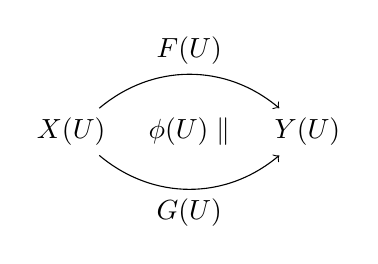
\begin{tikzpicture}
            % Nodes for X(U) and Y(U)
            \node (X) at (0,0) {$\mathfrak{X}(U)$};
            \node (Y) at (3,0) {$\mathfrak{Y}(U)$};

            % Top curved arrow
            \draw[->] (X) to[bend left=40] node[above] {$F(U)$} (Y);

            % Bottom curved arrow
            \draw[->] (X) to[bend right=40] node[below] {$G(U)$} (Y);

            % Middle label
            \node at (1.5,0) {$\phi(U)\parallel$};
        \end{tikzpicture}
    \]
    subject to some compatibility conditions.
\end{definition}


\begin{definition}[Fiber product of $k$-stacks]
    Given two 1-morphisms $i_1: \mathfrak{X}_1 \to \mathfrak{Y}$ and $i_2: \mathfrak{X}_2 \to \mathfrak{Y}$ of $k$-stacks, the \textbf{fiber product} $\mathfrak{X}_1 \times_{\mathfrak{Y}} \mathfrak{X}_2$ is the $k$-stack defined by the rule
    \[
        (\mathfrak{X}_1 \times_{\mathfrak{Y}} \mathfrak{X}_2)(V) = \set{(x_1, x_2, \alpha) | x_i \in \mathfrak{X}_i(V), \alpha: i_1(x_1) \xrightarrow{\sim} i_2(x_2) \text{ in } \mathfrak{Y}(V)}
    \]
\end{definition}

\begin{lemma}[The 2-Yoneda Lemma]\label{lemma:2yoneda}
Let $\mathfrak{X}$ be a prestack over a category $\mathcal{S}$ and $S \in \mathcal{S}$.
The functor
\[
\operatorname{Mor}(S,\mathfrak{X}) \;\longrightarrow\; \mathfrak{X}(S),
\qquad
f \longmapsto f_S(\mathrm{id}_S)
\]
is an equivalence of categories, where $\operatorname{Mor}(S,\mathfrak{X})$ is the category of 1-morphisms from the representable prestack $S$ to $\mathfrak{X}$.
\end{lemma}

\begin{definition}[Representable morphisms of $k$-stacks]
    Let $F: \mathfrak{X} \to \mathfrak{Y}$ be a morphism of $k$-stacks. Let $U \in \ob(\mathbf{Aff}/k)$ and $\eta \in \ob\mathfrak{Y}(U)$. In particular, by the 2-Yoneda lemma, such an object $\eta$ can be thought of as a morphism $\eta: U \to \mathfrak{Y}$, where we identify $U$ with the stack it represents.

    We define the fiber stack $\mathfrak{X}_\eta$ to be the fiber product of the two morphisms $F: \mathfrak{X} \to \mathfrak{Y}$ and $\eta: U \to \mathfrak{Y}$. Consider a test scheme $T$. Since $U$ is representable, $U(T)=\mathrm{Hom}(T,U)$, so $u$ is a map $u:T\to U$. The composite $\eta\circ u:T\to\mathcal Y$ is exactly the pullback of $\eta$ along $u$. We denote this object of $\mathcal Y(T)$ by $\eta_T$. Unwinding, we see that the objects of $\mathfrak{X}_\eta$ over a test scheme $T$ \begin{align*}
        \mathfrak{X}_\eta(T) = \set{(x, \alpha) | x \in \mathfrak{X}(T), \alpha: F(x) \xrightarrow{\sim} \eta_T \text{ in } \mathfrak{Y}(T)}
    \end{align*}

    The morphism $F: \mathfrak{X} \to \mathfrak{Y}$ is \textbf{representable} if $\mathfrak{X}_\eta$ is representable as a scheme for all $U \in \ob(\mathbf{Aff}/k)$ and all $\eta \in \ob\mathfrak{Y}(U)$.

    We say \textbf{$F$ has property $P$} if for every $U \in \ob(\mathbf{Aff}/k)$ and every $\eta \in \ob(\mathfrak{Y}(U))$ the canonical morphism (coming from forming the fiber stack as a pullback) of schemes $\mathfrak{X}_\eta \to U$ has $P$.  Examples of such properties are flat, smooth, surjective, étale, etc.
\end{definition}

\begin{definition}[Algebraic spaces and stacks]\label{def:algstack}
Let $\mathcal{F}$ be a sheaf on $\mathbf{Aff}/k$. We say $\mathcal{F}$ is an \textbf{algebraic space} if
\begin{enumerate}
    \item For any $U \in \operatorname{Ob}(\mathbf{Aff}/k)$, the morphism
    $U \to \mathcal{F}$ is representable by schemes, equivalently
    the diagonal
    \[
    \Delta : \mathcal{F} \longrightarrow \mathcal{F} \times \mathcal{F}
    \]
    is representable by schemes;
    \item There exists an \'etale surjective covering
    $\{ U_i \to \mathcal{F} \}$ with $U_i \in \operatorname{Ob}(\mathbf{Aff}/k)$.
\end{enumerate}

Let $\mathfrak{X}$ be a stack on $\mathbf{Aff}/k$.
We say $\mathfrak{X}$ is an \textbf{algebraic stack} if
\begin{enumerate}
    \item For any $U \in \operatorname{Ob}(\mathbf{Aff}/k)$, the morphism
    $U \to \mathfrak{X}$ is representable by algebraic spaces, equivalently
    the diagonal
    \[
    \Delta : \mathfrak{X} \longrightarrow \mathfrak{X} \times \mathfrak{X}
    \]
    is representable by algebraic spaces;
    \item There exists a smooth surjective covering
    $\{ U_i \to \mathfrak{X} \}$ with $U_i \in \operatorname{Ob}(\mathbf{Aff}/k)$.
\end{enumerate}
\end{definition}

\begin{remark}
    Some authors require that the diagonal morphism be separated and quasi-compact (and possibly other adjectives) as part of the definition of an algebraic stack. It appears that this is a technical condition that is not strictly necessary in most applications, so we omit it here.
\end{remark}

\begin{remark}
In some papers it is required that there exists a scheme $U$ and a surjective and étale morphism $U \to \mathfrak{X}$. In the paper where algebraic stacks were first introduced, Deligne and Mumford used this definition and showed that the moduli stack of stable genus $g>1$ curves is an algebraic stack which has an étale covering by a scheme.

    Michael Artin realized that many natural results on algebraic stacks generalize to the case where one only assumes a smooth covering by a scheme, as in the definition of algebraic stack above. The term "Deligne-Mumford stack" is used to indicate those algebraic stacks which have an étale covering by a scheme. However, the term Artin stack is reserved for another object.
\end{remark}

\begin{definition}
    An algebraic stack $\mathfrak{X}$ is a \textbf{Deligne-Mumford stack} if there exists an étale surjective covering $\{ U_i \to \mathfrak{X} \}$ with $U_i \in \operatorname{Ob}(\mathbf{Aff}/k)$.
\end{definition}

\begin{remark}
    Given any scheme $T$ with two maps $f, g : T \to \mathfrak{X}$ (representing two families of objects parameterized by $T$), the fiber product:
    \begin{align*}
        T \times_{(\mathfrak{X} \times \mathfrak{X})} \mathfrak{X} \cong \text{Isom}_T(f, g)
    \end{align*}
    represents the "scheme of isomorphisms" between the objects corresponding to $f$ and $g$.    The condition that $\Delta : \mathfrak{X} \to \mathfrak{X} \times \mathfrak{X}$ is representable means that for any scheme $T$ with a morphism $T \to \mathfrak{X} \times \mathfrak{X}$, the fiber product $T \times_{\mathfrak{X} \times \mathfrak{X}} \mathfrak{X}$ is (represented by) an algebraic space. This controls the "size" of automorphism groups.
\end{remark}

\subsection{Algebraic spaces vs algebraic stacks}
The difference between algebraic spaces and algebraic stacks is a little subtle. The best way to understand it is by introduce etale groupoids.

\begin{definition}
    An \textbf{étale groupoid} of schemes is a pair of schemes $(U, R)$ together with morphisms
    \[
        s, t: R \to U, \quad e: U \to R, c: R \times_{s, U, t} R \to R\]
        called source, target, and composition so that one has associativity, identity, and inverse axioms mimicking those of a groupoid. 

        If $(s,t): R \to U \times U$ is a monomorphism, we say the pair forms an \textbf{étale equivalence relation}.
\end{definition}

\begin{definition}[Quotient stack of a smooth groupoid]\label{def:quotient-stack-groupoid}
Let $s,t : R \rightrightarrows U$ be a smooth groupoid of algebraic spaces.
Define $[U/R]^{\mathrm{pre}}$ as the prestack whose objects over a scheme $T$ are morphisms
$T \to U$, and where a morphism $(a:S\to U) \to (b:T\to U)$ is the data of a morphism
$f:S\to T$ and an element $r\in R(S)$ such that $s(r)=a$ and $t(r)=f\circ b$.
Define $[U/R]$ to be the stackification of $[U/R]^{\mathrm{pre}}$ in the big
\'etale topology $\Sch_{\text{et}}$.
If in addition $R \rightrightarrows U$ is an equivalence relation, then $[U/R]$
is isomorphic to a sheaf (Exercise~3.4.12), and we denote it by $U/R$.

The fiber category $[U/R]^{\mathrm{pre}}(T)$ is the groupoid whose objects are
$U(T)$ and whose morphisms are $R(T)$.
The identity morphism $\mathrm{id}_U:U\to U$ defines a map $U\to [U/R]^{\mathrm{pre}}$
and therefore a map $p:U\to [U/R]$.
\end{definition}



\begin{theorem}[Algebraicity of Quotients by Groupoids]\label{thm:3.4.13}
\leavevmode
\begin{enumerate}
\item
If $R \rightrightarrows U$ is an \'etale \textup{(resp.\ smooth)} groupoid of algebraic
spaces, then $[U/R]$ is a Deligne--Mumford stack \textup{(resp.\ algebraic stack)}
and $U \to [U/R]$ is an \'etale \textup{(resp.\ smooth)} presentation.
\item
If $R \rightrightarrows U$ is an \'etale equivalence relation of schemes,
then $U/R$ is an algebraic space and $U \to U/R$ is an \'etale presentation.
\end{enumerate}
\end{theorem}

\begin{proposition}
    Let $X$ be an algebraic stack (resp., algebraic space) and let $U \to X$ be a smooth presentation. Then $X$ is isomorphic to the quotient stack $[U/R]$ (resp., the quotient sheaf $U/R$), where $R = U \times_X U$ is the fiber product and $R \rightrightarrows U$ is the étale groupoid (resp., equivalence relation) given by the two projections. 
\end{proposition}

\subsection{Algebraic stacks}
Let $G$ be a smooth affine group scheme of finite type over $k$ (equivalently, we can view $G$ as a representable sheaf of groups in Zariski topology). For instance, $G = \GL_n$ or $G = \Sp_{2n}$ or $G$ is any finite group scheme over $k$. Let $X$ be a fixed scheme over $k$.

\begin{definition}
    A \textbf{$G$-bundle} (or torsor) over $X$, by definition, is a sheaf $\mathcal P$ on $\mathbf{Aff}/k$ with a $G$-action 
$G \times \mathcal P \to \mathcal P$, such that there exists an étale cover $\{U_i \to X\}$ with 
$\mathcal P|_{U_i} \cong U_i \times G$ (as trivial $G$-bundles over $U_i$) and the $G$-action is locally trivial. 
Here for a $G$-action we mean that as a sheaf of sets, for the above cover $\{U_i \to U\}$, the map
\[
G(U_i) \times \mathcal P(U_i) \longrightarrow \mathcal P(U_i)
\]
is the usual group action in the set-theoretic sense.
\end{definition}

\begin{remark}
    When $G$ is smooth then a $G$-bundle in the étale topology is the same as a $G$-bundle in the fppf topology. 
If $G$ is not smooth (e.g.\ in positive characteristic), one must work with the fppf topology.
\end{remark}


\begin{remark}
    Using fpqc descent for affine morphisms, one can show that $\mathcal P$ is represented by an affine scheme over $X$. 
On the other hand, if $G$ is not affine, it can happen that a $G$-bundle is not representable by a scheme.
\end{remark}

\begin{definition}
    If $\mathfrak{X}$ is a prestack over a site $\mathcal{C}$, the \textbf{stackification} of $\mathfrak{X}$ is a stack $\mathfrak{X}^a$ together with a morphism of prestacks $\varphi: \mathfrak{X} \to \mathfrak{X}^a$ satisfying the following universal property: for any stack $\mathfrak{Y}$ and any morphism of prestacks $\psi: \mathfrak{X} \to \mathfrak{Y}$, there exists a unique morphism of stacks $\tilde{\psi}: \mathfrak{X}^a \to \mathfrak{Y}$ such that $\psi = \tilde{\psi} \circ \varphi$. In particular, the induced functor \begin{align*}
        \Hom(\mathfrak{X}^a, \mathfrak{Y}) \to \Hom(\mathfrak{X}, \mathfrak{Y})
    \end{align*} is an equivalence of categories.
\end{definition}


\begin{definition}
    Let $G$ be an algebraic group acting on a scheme $X$. The \textbf{action groupoid} $X/G$ is the category whose objects are the points of $X$ and morphisms from $x$ to $y$ are the elements of $G$ such that $gx = y$.
\end{definition} Note that the isomorphism classes of the action groupoid are in bijection with
the orbits of $G $ on $X$. There is a canonical map $X/G \to */G$ which is obvious on the level of groupoids.

\begin{definition}
    We define the \textbf{quotient prestack} $[X/G]^{\text{pre}}$ to be the category fibered in groupoids over $\Sch/k$, whose fiber over a test scheme $S$ is the action groupoid of $G(S)$ acting on $X(S)$.
\end{definition}

\begin{definition}
    We define the \textbf{quotient stack} $[X/G]$ to be the stackification of the quotient prestack $[X/G]^{\text{pre}}$. Its fiber over a test scheme $T$ is a groupoid whose objects are diagrams \begin{center}
    \begin{tikzcd}
        P \arrow[r] \arrow[d] & X \\
        T
    \end{tikzcd}
    \end{center}
    where $P \to T$ is a principal $G$-bundle, and $P\to X$ is a $G$-equivariant map. Morphisms between two such objects $(P \to T, P \to X)$ and $(P' \to T', P' \to X)$ are morphisms of principal $G$-bundles $P \to P'$ over $T \to T'$ which are compatible with the maps to $X$.
\end{definition}

\begin{proposition}
The quotient prestack $[X/G]^{\mathrm{pre}}$ is a stack (for the fppf topology).
\end{proposition}

\begin{proof}
Recall that $[X/G]^{\mathrm{pre}}(T)$ is the groupoid of pairs
\[
(P \to T,\; \phi:P\to X)
\]
where $P\to T$ is a principal $G$-bundle and $\phi$ is $G$-equivariant.  Morphisms are
$G$-equivariant maps of principal bundles over $T$ compatible with the maps to $X$.

Let $\{T_i \to T\}$ be an fppf covering.  Descent for objects and morphisms in
$[X/G]^{\mathrm{pre}}$ reduces to two standard facts.

First, principal $G$-bundles form a stack for the fppf topology:
the fibered category
\[
T \;\longmapsto\; \{\text{principal $G$-bundles on }T\}
\]
satisfies effective fppf descent. Unwinding, what this is saying is that a compatible system of principal $G$-bundles $P_i\to T_i$ with isomorphisms on $T_i\times_T T_j$ descends uniquely to a principal $G$-bundle $P\to T$.

Second, for any scheme (or algebraic space) $X$, the functor
$T\mapsto \Hom(T,X)$ is an fppf sheaf.  In particular, if
$\phi_i:P_i\to X$ are $G$-equivariant maps compatible with the descent data,
then they glue uniquely to a $G$-equivariant map $\phi:P\to X$.
\end{proof}

\begin{remark}
This definition is motivated by the following observation.
The first thing we notice is that the map $X \rightarrow *$ should induce a canonical map $X/G \rightarrow */G$. Thus an $S$-point of $S \rightarrow X/G$ induces by composition an $S$-point $S \rightarrow */G$; i.e., a $G$-torsor $P$ over $S$.

Now, say we have a $G$-torsor $P$ over $S$. We can form the fiber product:

\begin{center}
    \begin{tikzcd}
        X \times^G P \arrow[r] \arrow[d] & X/G \arrow[d] \\
        S \arrow[r, "P"] & */G
    \end{tikzcd}
\end{center}

We call the stack $X \times^G P$ the $X$-bundle associated to $P$, or the associated bundle of $P$ with
fiber $X$.
\end{remark}
In particular, there is the following correspondence:

\begin{proposition}
    There is a canonical bijection between:

    \begin{enumerate}
        \item Maps from a scheme $S$ to the quotient stack $X/G$
        \item Sections of the associated bundle $S \to X \times^G P$
        \item $G$-equivariant maps from $P$ to $X$
    \end{enumerate} where $P$ is the principal $G$-bundle on $S$ corresponding to $S \to X/G \to */G$.
\end{proposition}

\begin{proof}
    A map $f: S \to X/G$ of stacks corresponds to a principal $G$-bundle $P$ on $S$ together with a $G$-equivariant map $\phi: P \to X$. Given a $G$-equivariant map $\phi: P \to X$, we can construct a section $\sigma: S \to X \times^G P$ of the associated bundle as follows:

    For each point $s \in S$, define $\sigma(s) = [\phi(p), p]$ where $p$ is any point in the fiber $P_s$ and $[\phi(p), p]$ denotes the equivalence class in $X \times^G P$. The $G$-equivariance of $\phi$ ensures this is well-defined regardless of which $p \in P_s$ we choose.


    Conversely, given a section $\sigma: S \to X \times^G P$ where $\sigma(s) = [x_s, p_s]$ for each $s \in S$, we can define a $G$-equivariant map $\phi: P \to X$ as follows:

    For any $p \in P$ with $p \in P_s$ for some $s \in S$, we have $p = p_s \cdot g$ for some $g \in G$. We define $\phi(p) = g^{-1} \cdot x_s$. The properties of the associated bundle ensure this is well-defined and $G$-equivariant.
\end{proof}


\begin{theorem}[Algebraicity of Quotient Stacks]
If $G \to S$ is a smooth affine group scheme acting on a scheme $U \to S$, then the quotient stack $[U/G]$ is an algebraic stack over $S$ such that 
\[
U \to [U/G]
\]
is a principal $G$-bundle and in particular surjective, smooth, and affine. 
In particular, the classifying stack $BG = [S/G]$ is algebraic.
\end{theorem}

\begin{proof}
There is an object of $[X/G]$ over $X$ given by the diagram
\[
\begin{tikzcd}
G \times X \arrow[r, "\sigma"] \arrow[d, "p_2"'] & X \\
X &
\end{tikzcd}
\]
where $\sigma$ denotes the action map. 
By the 2--Yoneda Lemma, this defines a map 
\[
X \longrightarrow [X/G]
\]
Even if the action of $G$ on $X$ is not free, the map $X \to [X/G]$ is a principal $G$-bundle. 


We need to show that $U \to [U/G]$ is a principal $G$-bundle (meaning that for any morphism $T \to [U/G]$, the base change $U \times_{[U/G]} T \to T$ is a principal $G$-bundle).
let $T \to [U/G]$ be a morphism from an $S$-scheme 
classified by a principal $G$-bundle $P \to T$ 
and a $G$-equivariant map $P \to U$. 
Then there is a Cartesian diagram
\[
\begin{tikzcd}
P \arrow[r] \arrow[d] & U \arrow[d] \\
T \arrow[r] & {[U/G]}
\end{tikzcd}
\]
and since every base change is a principal $G$-bundle, 
so is $U \to [U/G]$.


We check that the fiber product $P$ is a scheme so that $U \to [U/G]$ is representable by schemes.

By definition, there exists an fppf cover $\{U_i \to T\}$ such that $\mathcal{P}|_{U_i} \cong U_i \times_S G$ as $G$-spaces. Each $U_i \times_S G$ is a scheme, affine over $U_i$, since $G$ is affine. On overlaps $U_{ij} = U_i \times_T U_j$, the identifications give isomorphisms of $G$-spaces
\[
\phi_{ij} : (U_i \times_S G)|_{U_{ij}} \xrightarrow{\sim} (U_j \times_S G)|_{U_{ij}}
\]
satisfying the cocycle condition on triple overlaps, because $\mathcal{P}$ is a sheaf.

Therefore, you have descent data for affine morphisms over $T$. By fpqc/fppf descent for affine morphisms (equivalently, for quasi-coherent algebras), there exists an affine $T$-scheme
\[
P \to T
\]
together with isomorphisms
\[
P \times_T U_i \cong U_i \times_S G
\]
compatible with the $\phi_{ij}$. These glue the $G$-action as well, so $P$ represents $\mathcal{P}$ and is a principal $G$-bundle in the usual scheme sense.

We also check that $P \to T$ is smooth (resp. étale) if $G \to S$ is smooth (resp. étale).

If $G\to S$ is smooth and $P\to T$ is a principal $G$-bundle, then there exists an
fppf cover $U\to T$ with $P\times_T U \cong U\times_S G$. The projection
$U\times_S G\to U$ is smooth as it is the base change of $G\to S$. Smoothness is preserved under base change and local on
the base in the fppf topology. Hence $P\to T$ is smooth.
\end{proof}

\begin{definition}[Stack of principal $G$-bundles]
An object of $\Bun_{G,X}$ over $S \in \mathrm{Aff}$ is a principal $G$-bundle on $X_S := X \times S$. Concretely, this means a morphism $\pi: P \to X_S$ with a right $G$-action, such that $P \to X_S$ is locally trivial in the specified topology.

The fiber category over $S$, written $\Bun_{G,X}(S)$, is
\[
\Bun_{G,X}(S)
= \left\{ \text{principal $G$-bundles on } X_S \right\}.
\]

Given objects $(S_1, P_1)$ and $(S_2, P_2)$, a morphism
\[
(S_1, P_1) \longrightarrow (S_2, P_2)
\]
is a pair $(f, \Phi)$ where $f: S_1 \to S_2$ is a morphism of schemes, and $\Phi: P_1 \to P_2$ is a $G$-equivariant morphism of schemes over $X$ covering $f$, such that the diagram
\[
\begin{tikzcd}
P_1 \arrow[r, "\Phi"] \arrow[d] & P_2 \arrow[d] \\
X_{S_1} \arrow[r, "id_X \times f"] & X_{S_2}
\end{tikzcd}
\]
commutes.

Pullbacks (cartesian morphisms) are given as follows: given $f: S_1 \to S_2$ and an object $P_2$ over $S_2$, its pullback along $f$ is the usual base-changed bundle
\[
f^*P_2 := P_2 \times_{X_{S_2}} X_{S_1} \to X_{S_1}.
\]
The canonical map $f^*P_2 \to P_2$ over $f$ is cartesian. This makes $\Bun_{G,X}$ a category fibered in groupoids in the standard way.

Every morphism in each fiber is an isomorphism. Fix a base $S$, so we are in the fiber $\Bun_{G,X}(S)$, whose objects are principal $G$-bundles $P \to X_S$, and morphisms are $G$-equivariant maps $P_1 \to P_2$ over $X_S$.

We claim that any such morphism is an isomorphism. This is fppf-local on $X_S$, so we may pick an fppf or étale cover $\{ U_i \to X_S \}$ trivializing both bundles:
\[
P_1|_{U_i} \cong U_i \times G, \qquad P_2|_{U_i} \cong U_i \times G.
\]
Over $U := U_i$, a $G$-equivariant map
\[
\phi: U \times G \to U \times G
\]
commuting with projection to $U$ must have the form
\[
\phi(u, g) = (u, g \cdot h(u))
\]
for a unique map $h: U \to G$. This map is invertible, with inverse
\[
(u, g) \mapsto (u, g \cdot h(u)^{-1}),
\]
so $\phi$ is an isomorphism. Thus, our original $G$-equivariant map is an isomorphism on each $U_i$. If $f:X\to Y$ is a morphism of schemes and there exists a surjective fpqc/fppf morphism
$Y’\to Y$ such that the base change $f’:X\times_Y Y’\to Y’$ is an isomorphism,
then $f$ is an isomorphism.

Therefore, every morphism in the fiber $\Bun_{G,X}(S)$ is invertible.
\end{definition}

Indeed $\mathrm{Bun}_{G,X}$ is a stack. 
The prestack structure is clear by functoriality of pullback, 
and the gluing condition follows from descent theory for fppf sheaves. When $X = \mathrm{Spec}\,k$, we denote it by $BG$, also written as $[*/G]$.

\begin{proposition}[Algebraic stack of principal $G$-bundles]\label{prop:algebraic_stack_principal_bundles}
    Let $X$ be a smooth projective curve over $k$ of genus $g$ and $G$ is reductive. The stack $\Bun_{G,X}$ is smooth, dimension $\dim G(g-1)$.
\end{proposition}

\begin{proof}
Recall that given any principal $G$-bundle $E \to X$ and a representation $V$ of $G$, you can form the associated vector bundle $E(V) := E \times^G V$. This is the quotient of $E \times V$ by the right $G$-action $(e, v) \sim (eg, g^{-1}v)$.

In particular, for the adjoint representation $V = \mathfrak{g}$, we have
\[
E(\mathfrak{g}) := E \times^G \mathfrak{g}
\]
is a vector bundle on $X$ whose fibers are copies of the Lie algebra $\mathfrak{g}$, twisted by the bundle $E$.

    The geometry of this stack is controlled by deformation theory and in particular the cohomology groups of these adjoint bundles. Given a principal $G$-bundle $E$ over $X$: \begin{itemize}
        \item The infinitesimal automorphisms of $E$ are given by $H^1(X, E(\mathfrak{g}))$ where $E(\mathfrak{g})$ is the adjoint bundle associated to $E$.
        \item Automorphisms of $E$ are given by $H^0(X, E(\mathfrak{g}))$.
        \item The obstructions to deformations of $E$ lie in $H^2(X, E(\mathfrak{g}))$. Since $X$ is a curve, this group is zero.
    \end{itemize}
    In particular, this shows that the moduli stack is smooth. \red{For algebraic stacks, we have the tangent complex formalism which reduces to the following:}
    \begin{align*}
        T_{\mathcal{M}_{G,X}}|_{[E]} & = R\Gamma(X, E(\mathfrak{g}))[1] \\
        \mathbb{L}_{\mathcal{M}_{G,X}}|_{[E]} & = R\Gamma(X, E(\mathfrak{g}))^*[-1].
    \end{align*}
\red{At the point corresponding to $E$, we have}:
    \[\dim T_{[E]} \mathcal{M}_{G,X} = \dim H^1(X, E(\mathfrak{g})) - \dim H^0(X, E(\mathfrak{g})) = -\chi(X, E(\mathfrak{g}))\]

Since $\deg(E(\mathfrak{g})) = 0$ and $\operatorname{rk}(E(\mathfrak{g})) = \dim(G)$, we have by Riemann-Roch:
    \[
    \chi(X, E(\mathfrak{g})) = \operatorname{rk}(E(\mathfrak{g}))(1-g) = \dim(G)(1-g)
    \]
    Therefore:
    \[
    \dim \mathcal{M}_{G,X} = \dim(G)(g-1)
    \]
\red{See Sam Raskin notes}
\end{proof}

\begin{proposition}[Line bundles on quotient stacks]
\label{prop:Pic_quotient_stack}
Let $S$ be a base scheme, $H$ a flat group scheme of finite type over~$S$, 
and $Y$ an algebraic space (or scheme) equipped with an $H$–action.
Denote by $[Y/H]$ the corresponding quotient stack, and let
\[
\pi : Y \longrightarrow [Y/H]
\]
be the natural projection.

Then pullback along~$\pi$ induces a canonical isomorphism
\[
\pi^* : \Pic([Y/H]) \xrightarrow{\;\sim\;} \Pic_H(Y),
\]
where $\Pic_H(Y)$ denotes the group of $H$–linearized line bundles on~$Y$.

\end{proposition}

\begin{proof}[Sketch of proof]
A line bundle $\mathcal L$ on the quotient stack $[Y/H]$ is, by definition,
a line bundle on $Y$ together with descent data relative to the covering
$\pi : Y \to [Y/H]$.
Unwinding the descent condition gives an isomorphism
\[
m^*\mathcal L \;\simeq\; pr_2^*\mathcal L
\quad\text{on } H\times Y,
\]
compatible with the cocycle condition on $H\times H\times Y$.
This is precisely the definition of an $H$–linearization of~$\mathcal L$.
Conversely, any $H$–linearized line bundle on~$Y$ descends uniquely
to a line bundle on the quotient stack.
Hence $\pi^*$ is an isomorphism.
\end{proof}


\section{References}
\begin{enumerate}
        % alper book
    \bibitem{alper}
    Alper, J., Stacks and moduli,
    \url{https://sites.math.washington.edu//~jarod/moduli.pdf}


    \bibitem{BeauvilleLaszlo1994}
    Beauville, A., and Laszlo, Y.,
    "Conformal blocks and generalized theta functions,"
    \textit{Communications in Mathematical Physics},
    vol. 164, no. 2, pp. 385--419, 1994.

    \bibitem{descent}
    Behrend, Conrad, Edidin, Fantechi, Fulton, Gottsche, and Kresch's notes on DM stacks.\url{https://math.colorado.edu/~casa/seminars/reading/stack_of_curves_21/papers/fultonetalstacks/6AfultonAppDescent.pdf}

        \bibitem{EGA}
    Grothendieck, A.,
    \textit{Éléments de géométrie algébrique (EGA)},
    Publications Mathématiques de l'IHÉS, vol. 4, 1960.

        % mukai book

    \bibitem{Olsson2016}
    Olsson, M. C.,
    \textit{Algebraic Spaces and Stacks},
    American Mathematical Society Colloquium Publications, vol. 62,
    American Mathematical Society, Providence, RI, 2016.

    \bibitem{Sorger1999}
    Sorger, C.,
    "Lectures on moduli of principal $G$-bundles over algebraic curves,"
    in \textit{School on Algebraic Geometry (Trieste, 1999)}, pp. 1--57,
    ICTP Lecture Notes, vol. 1, Abdus Salam International Centre for Theoretical Physics, Trieste, 1999.


\end{enumerate}
\end{document}